\documentclass{article}
\usepackage{natbib}
\usepackage{multirow}
\usepackage{booktabs}
\usepackage{changepage}
\usepackage{caption} % For caption customization
\usepackage{lineno} % For line numbers
\usepackage{graphicx} % For including graphics
% Add line numbers to the document
\usepackage{geometry}


%\usepackage{hyperref}
\usepackage[colorlinks = true, linkcolor=blue, urlcolor=blue, citecolor=blue]{hyperref}
\usepackage[nameinlink]{cleveref}
\crefname{figure}{Fig.}{Figs.}

\linespread{2} 

{\Large 
	\title{Spatio-temporal variability of zooplankton standing stock in eastern Arabian Sea inferred from ADCP backscatter measurements }}
\author{Ranjan Kumar Sahu, P. Amol, D.V. Desai, S.G. Aparna,  D. Shankar}
\date{\today}
\begin{document}
	

	\maketitle
	\linenumbers
	\section*{Abstract}
	
We use acoustic Doppler current profiler (ADCP) backscatter measurements to map
the spatio-temporal variation of zooplankton standing stock in the eastern Arabian Sea (EAS). The ADCP moorings were deployed at seven locations on the continental slope off the west coast of India; we use data from October 2017 to December 2023. The 153.3 kHz ADCP uses backscatter from sediments or organisms such as copepods, ctenophores, salps and amphipods greater than 1 cm to calculate current profile. The backscatter is obtained from echo intensity using RSSI conversion factor after doing necessary calibrations. The conversion from backscatter to biomass is based on volumetric zooplankton sampling at the respective locations. Analysis of the data over 24 – 120 m shows that the backscatter and zooplankton biomass decrease from the upper ocean (215 $m\ g^{-3}$ biomass contour) to the lower depths. Changes are observed in the seasonal variation of the monthly climatology of zooplankton standing stock (integral of the biomass over 24 – 120 m water
column) as we move to poleward along the slope in EAS. The range of variation of standing stock is lowest at Kanyakumari, followed by Okha, which lie at the southern and northern boundary of the EAS, respectively. Complementary variables are used to explain the processes leading to growth or decay of zooplankton biomass.	
	\newpage
	\section{Introduction}
	\subsection{Background}
	Zooplankton plays a vital role in food web of pelagic ecosystem by enabling the hierarchical transport of organic matter from primary producers to higher trophic levels impacting the fish population and the carbon pump of the deep ocean \citep{ohman2001density, le2016global}. They are presumably the largest migrating organisms in terms of biomass \citep{hays2003review} which occurs in diel vertical migration (DVM). Zooplanktons depend not only on phytoplankton but other environmental parameters (e.g. Mixed layer depth, insolation, Oxygen, thermocline, nutrient availability, chlorophyll concentration and daily primary production). The biological productivity of the ocean is essentially connected with physics and chemistry \citep{subrahmanyan1959studiespart2, ryther1966primary, qasim1977biological, nair1970primary,banse1995zooplankton,mccreary2009biophysical, vijith2016consequences,amol2020modulation}. The dynamic ocean results in varying physico-chemical properties, leading to bloom and growth of planktons in favourable conditions. The changes are strongly influenced by the seasonal cycle in the North Indian Ocean (NIO; north of ~5 $^o$N of Indian Ocean). The eastern boundary of Arabian Sea contains the West India Coastal Current (WICC; \citep{patil1964hydrography, ramamirtham1965hydrography, banse1968hydrography,shetye1991coastal, mccreary1993numerical, shankar1997dynamics, shetye1998coastal, maheswaran2000upwelling, schott20011,  amol2014observed, chaudhuri2020observed,chaudhuri2021observed}) which reverses seasonally, flowing poleward (equatorward) during November to February (June to September). 
	
	The direct consequence of this reversal is the seasonal cycle of thermocline, oxycline and thickness of mixed Layer Depth (MLD) induced by upwelling favourable conditions in summer and downwelling favourable conditions in winter in eastern Arabian Sea (EAS). Further, the phytoplankton biomass and chlorophyll concentration changes with the season \citep{subrahmanyan1960studies, banse1968hydrography, levy2007basin, vijith2016consequences}. Upwelling in  summer monsoon leads to maximum chlorophyll growth in the entire EAS \citep{ banse1968hydrography, banse2000geographical, mccreary2009biophysical, hood2017biogeochemical,shi2022phytoplankton}. During winter monsoon, the convective mixing induced winter mixed layer \citep{shetye1992does, madhupratap1996mechanism, levy2007basin, vijith2016consequences, shankar2016inhibition, keerthi2017physical,shi2022phytoplankton} results in winter chlorophyll peak in northern EAS (NEAS) while the downwelling Rossby waves modulate chlorophyll along the southern EAS (SEAS) albeit limited to coast and islands \citep{amol2020modulation}. 
	
	The zooplankton grazing peak is instantaneous with no time delay from peak phytoplankton production \citep{li2000determines,barber2001qn}, but its population growth lags \citep{rehim2012dynamical, almen2020temperature} depending on its gestation period and other limiting aspects. While some studies suggest that the peak timing of zooplankton may not change in parallel with phytoplankton blooms \citep{winder2004climatic}, others indicate that lag exists between primary production and the transfer of energy to higher trophic levels \citep{brock1992interannual, brock1991phytoplankton}. In their work, \citet{aparna2022seasonal} (A22 from hereon) had shown that peak zooplankton population may never occur even with a bloom in phytoplankton such as in SEAS, leading to the collapse of ecological models and succeeding food webs of higher trophic levels.  
	
	The conventional zooplankton measurements, where only few snapshot/s of the event is captured gives an incoherent or incomplete understanding in terms of spatio-temporal variation of zooplankton \citep{ramamurthy1965studies, piontkovski1995spatial, madhupratap1992zooplankton,madhupratap1996lack,wishner1998mesozooplankton,kidwai2000dd,barber2001qn,khandagale2022seasonal} as much information is revealed by later studies \citep{jyothibabu2010re, vijith2016consequences, shankar2019role, aparna2022seasonal} using high resolution data. Calibrated acoustic instruments such as Acoustic Doppler Current Profiler (ADCP) along with relevant data can be utilised to understand small scale variability \citep{nair1999arabian, edvardsen2003assessing, smith2005mesozooplankton, smeti2015spatial, kang2024acoustic}, the complex interplay between the physico-chemical parameters and ecosystem \citep{jiang2007temporal, potiris2018acoustic, shankar2019role, aparna2022seasonal, nie2023influence}, the zooplankton migration \citep{inoue2016diel,ursella2018evidence, ursella2021diel} and their seasonal to annual variation \citep{jiang2007temporal, hobbs2021marine,liu2022seasonal, aparna2022seasonal}.
	
	\subsection{ADCP backscatter and zooplankton biomass}
	At present, there are two types of acoustic samplers: non-calibrated single frequency acoustic profiler such as ADCP or calibrated multi and mono frequency acoustic profilers such as zooplankton acoustic profiler (ZAP) and Tracor acoustic profiling system(TAPS). The use of acoustics as a proxy for zooplankton biomass estimation can be traced to \citet{pieper1971study, sameoto1977use} and earlier studies which used echograms to approximate the large-scale horizontal extents \citep{barraclough1969shallow}, and small scale vertical extent \citep{mcnaught1968acoustical}. The relationship between backscatter and the abundance and size of zooplankton was described by \citet{greenlaw1979acoustical} 
	wherein it was pointed out that single frequency backscatter can be used to estimate abundance if mean zooplankton size is known. This paved the way for use of single frequency acoustic profiler. A drastic increase in study temporal and spatial variation of zooplankton biomass using  backscatter-proxy came in 1990s by introduction of high frequency echo sounders, with studies \citep{flagg1989use, wiebe1990sound, batchelder00981, greene1998three, rippeth1998diur} methodically showing acoustic backscatter estimated zooplankton biomass in various shelf and slope locations around  North Atlantic, North pacific location. The foundation for further research that investigated the potential of acoustic backscatter from ADCPs and multi frequency echo sounders in assessing zooplankton biomass and comprehending zooplankton dynamics in diverse maritime habitats was established by these initial explorative experiments.
	
	Acoustic backscatter and zooplankton biomass have been better understood as a result of technological and methodological developments over time. Net sampling augmented ADCP backscatter have been used to study DVM and the spatial and temporal variability of zooplankton biomass in different marine regions, such as the Southwestern Pacific, the Lazarev Sea in Antarctica and the Corsica Channel in the north-western Mediterranean Sea \citep{cisewski2010seasonal,hamilton2013links,smeti2015spatial, guerra2019zooplankton}.	The zooplankton biomass variation in the Arabian sea has been studied during JGOFS programme in 1990s \citep{herring1998across, nair1999arabian, barber2001qn,fielding2004biological, smith2005mesozooplankton}. However, their studies were limited to the cruise duration as vessel mounted ADCPs were predominantly used; hence long-term data was sparsely produced. The first such study to fully exploit the immense potential of ADCPs in EAS was carried out by A22 using ADCP moorings deployed on continental slopes off the Indian west coasts \citep{amol2014observed, chaudhuri2020observed}. A fascinating outcome of A22 is the non-linear interaction between zooplankton and phytoplankton population. A22 showed that the zooplankton growth in fact declines during upwelling facilitated increase in phytoplankton biomass. It implies the break down of existing understanding of predator - prey relationship in fundamental level of marine food chain with secondary production as a linear function of primary production.
	
	
	\subsection{Objective and scope of the manuscript}
	
	A network of ADCPs has been installed off the continental slope and shelf on the west coast of India. This ADCPs have enabled a rigorous view of intraseasonal to seasonal scale variability \citep{amol2014observed, chaudhuri2020observed}. Initially a network of four ADCPs (off Mumbai, Goa, Kollam and Kanyakumari) on continental slope, it has been extended to include three more moorings (off Okha from 2018, Jaigarh and Udupi from 2017). In the recent study A22 have used ADCP moorings off  Mumbai, Goa and Kollam to explain the temporal variability of zooplankton biomass. The study showed that the zooplankton peaks (and troughs) is not only non-uniform in latitude but also heavily influenced by the oxygen minimum zone, MLD and the seasonal upwelling/downwelling conditions. Stark contrast in the phytoplankton bloom and subsequence  growth of zooplankton or the lack thereof was observed in the EAS regimes.

	We build upon the existing work by extending to include the newly incorporated ADCPs so as to have a better understanding in the latitudinal variation of zooplankton biomass in EAS. The paper is organized as follows; datasets and methods employed are described in detail in section 2. Section 3 describes the observed climatology of zooplankton biomass and standing stock. A comparison is drawn to the results of previous studies at the overlapping mooring sites. Further, the seasonal cycle of zooplankton biomass and standing stock is discussed. The role of mixed layer depth, net primary production, sea surface temperature, wind forcing and circulation in determining the biomass is discussed in results section 4, with conclusion in section 5.
	
	\section{Data and methods}
	The  backscatter data from ADCP and the zooplankton samples collected from the periphery of mooring is described in this section. The methodology followed in processing ADCP data and estimation of backscatter and subsequently the zooplankton biomass is discussed. The backscatter derived from the echo intensity of the seven ADCP mooring deployed on the continental slope off the Indian west coast is the primary data we have use in this manuscript. The moorings details are summarized in \autoref{tab:table1}. In situ biomass data from volumetric zooplankton samples are used to validate and correlate with backscatter. The chlorophyll data is obtained from \href{https://data.marine.copernicus.eu/products}{marine.copernicus.eu}. In addition, we have used the monthly climatology of temperature and salinity \citep{chatterjee2012new} and the net primary productivity from MODIS (Moderate Resolution Imaging Spectroradiometer) and VIIRS (Visible Infrared Imaging Radiometer Suite) from global NPP estimates (\href{http://sites.science.oregonstate.edu/ocean.productivity}{http://sites.science.oregonstate.edu/ocean.productivity}). 
	
	\subsection{ADCP data and Backscatter estimation}
	The ADCPs were deployed on the continental slope off the Indian west coast (\cref{fig:map}), off Mumbai, Goa, Kollam and Kanyakumari, and later extended to three more sites to cover the entire EAS basin from Okha (22.26$^o$N) in north to Kanyakumari (6.96 $^o$N) in south. The other two ADCPs are  Jaigarh at central EAS (CEAS) and Udupi in the transition zone between CEAS \& SEAS. The extended moorings were deployed in October 2017, except for Kanyakumari which was deployed earlier as well but it wasn't part of the earlier backscatter study by A22. The moorings are serviced on yearly basis usually during October-November or in winter monsoon months. The ADCPs are of RD Instruments make, upward-looking and operate at 153.3 kHz. While utmost care is taken to position the instrument at  $\sim$ 200 m depth, yet for some deployments it's shallow or deeper owing to drift caused by floater buoyancy-anchor weight balance. Data was collected at hourly interval and the bin size was set to 4 m. The echoes at surface to 10 \% range ($\sim$ 20 m) means the data at these depths is rendered useless and is discarded from further use. 
	
	The procedure followed in processing of the ADCP data are described in \citet{amol2014observed} and \citet{mukherjee2014observed}. Depth correction was an addition to their methodology to accommodate the vertical movement of ADCP buoys \citep{chaudhuri2020observed, mukhopadhyay2020observed}
    using data from pressure sensor mounted on the instrument. We have followed the methodology laid down in A22 to derive the backscatter time series from ADCP echo intensity data which is discussed later paragraph. The gaps up to two days are filled using the grafting method of \citet{mukhopadhyay2020observed} once the zooplankton biomass time series is constructed.
    
	The primary objective of ADCP usage is to obtain vertical current profile at a point location. It is achieved by using the echo intensity received at the ADCP transducer. The instrument sensors doesn't directly give backscatter, as echo intensity is range independent. Range correction has to be performed before echo intensity (E) is converted to Backscatter (B). Received signal strength indicator (RSSI), also called the conversion factor (Kc) is sensor specific and is used with the corresponding reference echo intensity (Er). It's important to state that for the same device Kc remains unchanged while Er may vary over each subsequent deployment. The backscattering strength (in dB) is given by \citet{mullison2017backscatter}:
	
	$B = [C - L_{DBM}-P_{DBW}] + 2\alpha R + {10 log_{10}[(T_{TD}+273.16)R^2] } + {10log_{10} [10^{K_c(E-E_r)/10}-1]}$
	
	where $C$ is an empirical constant, $L_{DBM}$ is 10$log_{10}L$ where $L$ is the transmit pulse length in meters, $P_{DBW}$ is 10$log_{10}P$ ($P$ is  transmitted power in watts), $\alpha$ is the sound absorption coefficient of water (in $dB\ m^{-1}$),  $T_{TD}$ is the temperature (in $^o\ C$) at the depth of positioned instrument, $R$  is the slant range (in meters) from transducer to the scatterers and $E_r$ is	the reference level of $E$ taken in real-time (unit counts). $E_r$ in our case is taken from first (last) measured profile when the instrument is in air before (after) deployment (retrieval). The backscattering strength is referenced to ($4\pi m^{-1}$) \citep{deines1999backscatter, mullison2017backscatter}.  A22 has discussed the relevance of each of the term to the total backscattering strength. Our analysis also suggests that the $\alpha$ does not affect the final results. 
	
	\subsection{Zooplankton data and estimation of biomass}
	The  zooplankton  samples were collected in the vicinity ($\sim$ 10 km) of ADCP mooring site twice; once prior retrieval and again post deployment of moorings so that there is overlap in the ADCP time instance and in situ zooplankton samples. The sampling is done at the mooring location during servicing cruises on board RV Sindhu Sankalp and RV Sindhu Sadhana (Table 2). Multi-plankton net (MPN) (100 $\mu m$ mesh size, 0.5 $m^2$ mouth area) was used to get samples in the pre-determined depth ranges; water volume filtered was calculated by the product of sampling depth range and the mouth area of net. The depth range and timing of sample collection was different throughout the MPN hauls (refer \autoref{tab:table2}). From 2020 onward, the depth-range was standardized to the bins of 0 -- 25, 25 -- 50, 50 -- 75, 75 -- 100, 100 -- 150 (units are in meters). The collected zooplankton samples were then preserved in 5 \% formaldehyde solution until it's transferred to laboratory. To measure zooplankton wet weight accurately, the gelatinous forms/salps were separated. A22 had reported the calanoid copepods, cyclopoid copepods, Poecilostomatoida, Harpacticoida, appendicularians, euphausids, ostracods, and
	chaetognaths as the major groups of zooplanktons contributing to the biomass of net samples from the mooring sites. 
	The backscatter obtained earlier is averaged in vertical corresponding to the specific MPN hauls for each site. The backscatter is linear regressed with respective biomass to establish their relationship, which has been demonstrated in numerous previous studies \citep{flagg1989use,heywood1991estimation,jiang2007temporal,aparna2022seasonal}. 
	
	We calculated the regression equation to be $y$ = 0.0203 $x$  + 4.01 and, which is well within the error range of the regression equation of A22, $y$ = (0.02±0.004) $x$ + (4.14±0.36) with a correlation of 0.53 (\cref{fig:bstobm}). The correlation value in our case is 0.54; the minor difference is  due to higher number of data points (159) in the present study compared to A22 (67). 
	
	\subsection{Biomass time series and estimation of standing stock}
	
	The zooplankton biomass time series (\cref{fig:dailynmonthly}) is created from the above derived linear relationship: 
	
	$Bm$ = $m$ * $Sv$ + $k$ 
	
	where $Bm$ is biomass taken in log$_{10}$ scale, $m$ is slope, $Sv$ denotes  backscattering strength and $k$ is the intercept. The time series shows the pattern of diel vertical migration (DVM) at all the mooring sites during dawn ($\sim$0600-0700 hours) and dusk ($\sim$1800-1900 hours). It is evident in earlier studies using backscatter \citep{ashjian2002distribution, smith2005mesozooplankton, inoue2016diel,ursella2018evidence} and in situ zooplankton data \citep{padmavati1998vertical}. The implication of DVM is a higher biomass at surface during the night as zooplankton feeds and a lower biomass at daytime as they descend to subsurface depths. The overall biomass over the time period of a day may vary but the DVM doesn't affect the seasonal variation as shown by \citet{jiang2007temporal} and A22. Since our goal is to study the seasonal variation, delineating the daily biomass is sufficient. The biomass time series and it's seasonal cycle is discussed in \autoref{sec:seasonalcyclebiomass}.
	
	The standing stock is determined by taking the depth integral of biomass over the water column. To maintain the consistency of standing stock estimation, only those deployments that doesn't lack data at any depth in the entire range of 24 -- 120 m are considered for analysis as in A22. The lack of data in the above mentioned depth range is due to deviation in positioning of ADCP sensor in the water column. A swift alteration in bathymetry along the continental slope implies that the mooring might anchor at a different depth than planned, hence a change in the predicted position of ADCP. This leads to gap in data at few mooring sites for some year. For example, for the northern-most mooring at Okha, data is not available for the entire upper 120 m depth for the second deployment. Also at Jaigarh, where the surface to $\sim$60m data (in 3rd deployment) and Kollam, where 80 m and below (in 4th deployment) is unavailable and hence discarded from standing stock estimation. There are few deployments where no data or bad data was recorded e.g, at Udupi (4th deployment) and Kanyakumari (6th deployment). The seasonal cycle of standing stock for 24 -- 120 m available data is explored in \autoref{sec:seasonalcyclebiomass}.
	
	Through the findings of biomass variability in different time scale, we hypothesize that current may influence the zooplankton biomass by driving nutrients and phytoplankton rich water. Wavelet coherence between current and biomass is taken for each depth, and from this data, the coherence and phase at annual period is taken to check for dependency of biomass on current. In \autoref{vari} we shed a light on possible dependency of biomass on zonal \& meridional current.
	
	
	\subsection{Mixed-layer depth, temperature and oxygen}
	As we are using a 153.3 kHz ADCP moored at $\sim$ 150 m, the top $\sim$ 10\% of data is unusable because of surface echoes. MLD in EAS is of the order $\sim$ 20 to 40 m during summer monsoon \citep{shetye1990hydrography,sreenivas2008monthly} especially in the SEAS, but during winter the MLD in northern NEAS remains deep \citep{shankar2016inhibition}. Although it is possible to use the near-surface ADCP data after due noise correction; it is beyond the scope of present study. The temperature data is used from \citet{chatterjee2012new}, a monthly climatology having 1 $^o$ spatial resolution. Monthly climatology of oxygen data is obtained from World Ocean Atlas 2013 \citep{garcia2013oxygen} which contains objectively analyzed 1 $^o$ climatological fields of in situ measurements. 
	
	\subsection{Chlorophyll and net primary productivity data}
	Previous study based on ADCP data of EAS A22 have used SeaWIFS based chlorophyll data for comparison with climatology of zooplankton standing stock (ZSS). The SeaWIFS was at its end of service in 2010, hence we use new chlorophyll product. The present study has been conducted using Global Ocean Colour, biogeochemical, L3 data obtained from the  \href{https://doi.org/10.48670/moi-00280}{E.U. Copernicus Marine Service Information}. The daily data is available at a spatial resolution of 4 km. 

	%While chlorophyll is used to compare with the variation in climatology of zooplankton standing; the growth efficiencies of zooplankton are directly linked to primary production levels, emphasizing the interconnectedness between primary producers and consumers in marine food webs \citep{friedland2012pathways}. In their study, A22 has emphasized on the collapse of the predator-prey relationship between zooplankton-phytoplankton using climatological data. We showcase their interdependency or the lack thereof using net primary productivity models.
	%Moderate Resolution Imaging Spectroradiometer (MODIS) based net primary productivity (NPP) data at a resolution of 0.16$^o$ x 0.16$^o$ was obtained from Oregon State University. They have employed three different schemes to obtain NPP from Chlorophyll concentration. Those are discussed below in brief. The first is Vertically Generalized Production Model (VGPM). The NPP (a rate term) is to be derived from chlorophyll (a standing stock) using chlorophyll-specific assimilation efficiency for carbon fixation. The single biggest unknown in all models based on chlorophyll is how this rate term is described. VGPM considers the primary productivity to be dependent on day length and maximum daily NPP within a water column. The second is Carbon-based Productivity Model (CbPM) which NPP to phytoplankton carbon biomass and growth rate. The third is Carbon, Absorption, and Fluorescence Euphotic-resolving (CAFE) mode; first described in \citet{silsbe2016cafe} takes various other factors into NPP calculations. We explore these NPP models and try to explain the variation in ZSS.
	 
	\section{Climatology of zooplankton biomass and standing stock}
	The previous study of zooplankton in EAS based on ADCP backscatter was consisting of three sites: Mumbai in NEAS, Goa in CEAS and Kollam in SEAS. The extended mooring sites are at Okha at NEAS, Jaigarh at CEAS, Udupi in the transition zone of CEAS \& SEAS and Kanyakumari at SEAS is the southern most location in our study area. 

	ADCP data from three mooring sites were analysed from 2012 to 2020 in A22. They have fine-tuned the methodology to obtain backscatter and estimated zooplankton biomass from it using in situ volumetric zooplankton biomass data. A comparison is made in later paragraphs, since the methodology remains same in the current study and new time series data is available. The monthly climatology of biomass and ZSS is computed for all locations having valid data in 24 -- 140 m depth range (\cref{fig:zsschlclim}).
	 
% ommited out
%	The high biomass regime in the upper ocean and low biomass regime in deeper depths is differentiated using the 215 $mg\ m^{-3}$ biomass contour. For simplicity, this biomass contour is abbreviated to be z215 and its depth is denoted as D215 henceforth; region lying above this contour is the upper ocean biomass. The choice of 215 $mg\ m^{-3}$ isn't abrupt; it is carefully chosen to accommodate the seasonal variation, as a shift to biomass contour lower than the z215 would be unviable as our data is only till 140 m depth. A higher biomass contour would lead to inferior view of the seasonal cycle such as in the case of Kanyakumari and Okha where D215 is often low enough to reach $\sim$20 - 30 m depths. The climatology of zooplankton biomass at different mooring location is discussed at locations northward starting from southern mooring location (Fig. 4).
	

	The high biomass regime in the upper ocean and low biomass regime in deeper depths is differentiated using a biomass contour: 215 $mg \ m^{-3}$ off Mumbai, Goa, Kollam, Jaigarh and Udupi, 175 $mg \ m^{-3}$ off Okha and Kanyakumari. For simplicity, this biomass contour is abbreviated to be z215 \& z175 and its depth is denoted as D215 \& D175, respectively. The choice of biomass contour isn't abrupt; first, it is carefully chosen to accommodate the seasonal variation, as a shift to biomass contour lower than the z215 would be unviable as our data is only till 140 m depth, for example in the case of Kollam, the D215 exceeds 140 during few months of 2022 (\cref{fig:dailynmonthly}). A higher biomass contour would lead to inferior view of the seasonal cycle as in the case of Kanyakumari and Okha where 215 $mg \ m^{-3}$ biomass contour is often low enough to reach $\sim$20 -- 30 m depths, hence z175 is chosen here. Second, it allows us to link the seasonal variation of biomass to the physico-chemical properties.
	
	The climatology of zooplankton biomass and ZSS (\cref{fig:zsschlclim}) is discussed at locations northward starting from southernmost mooring site off Kanyakumari. 
	 
	\subsection{Southern EAS}
	During mid-march off Kanyakumari, the depth of 23 $^o$ C isotherm (henceforth D23) shallows along-with oxycline (marked by 2.1 $ml \ L^{-1}$) and a rise in biomass is observed (\cref{fig:zsschlclim} g1). The z175 is shallower from May onward to October and the zooplankton biomass is comparatively higher than rest of the year. The D175 deepens starting from October and the relatively high biomass in water column is maintained till late December. However, this increase in D175 isn't reflected as an increase in ZSS because of low biomass in the entire water column. A gradual increase is seen in the chlorophyll biomass starting from April and the peak is attained in June (\cref{fig:zsschlclim} g2). The ZSS is increased in June, however the growth is minimal. There is almost no seasonal variation in ZSS off Kanyakumari (ZSS std, 0.67 $gm\ m^{-2}$) as compared to the ZSS variation at the nearest northern mooring site off Kollam (ZSS std, 1.25 $gm\ m^{-2}$), where a strong seasonal cycle is observed and the D215 is deeper for any given month.
	
	Off Kollam, a higher biomass is present in the larger portion of water column and the D215 is at $\sim$ 110 m during Mar-May (\cref{fig:zsschlclim} f1). Similar to z175 off Kanyakumari, the decrease in biomass with depth is subtle below z215. Starting from March, the D215 begins to shallow with progress in time till August. During this period, a sharp decrease is seen in the D23 ($\sim$ 80 m in June to September) while the oxycline (1.7 $ml \ L^{-1}$) overshoots the thermocline (\cref{fig:zsschlclim} f1). A steep rise in chlorophyll biomass is seen off Kollam and its peak is attained in August (\cref{fig:zsschlclim} f2). The ZSS declines in the same period and reaches a minimum when the chlorophyll biomass is at its peak. The chlorophyll biomass decreases rapidly in the following months, while the ZSS increases and a maximum is seen during October. This feature was earlier reported by A22 showing disproportionate interaction between zooplankton and phytoplankton. A similar feature is seen further north, off Udupi which sits at the transition zone of SEAS \& CEAS, albeit with a relatively weaker zooplankton biomass. The peak of chlorophyll and minimum of ZSS occurs in September (\cref{fig:zsschlclim} e2) which is one month later than off Kollam. The 2.1 $ml \ L^{-1}$  oxygen contour overshoots thermocline, however it reaches to a much shallow depth of $\sim$ 20 m during July to October unlike any other location in our EAS study area. The D215 vaguely follows D23; with the gradual shallowing from March onward reaching $\sim$ 60 m in September and a steep decline afterwards till November (\cref{fig:zsschlclim} e1). The decrease of biomass with depth is moderate in comparison to Kollam.
	

	\subsection{Central EAS}
	Off Goa, the D215 seasonal trend is similar to Udupi and is entirely restricted by D23 \& 1.7 $ml \ L^{-1}$ oxygen contour that closely follows it. During March-May, the D215 is at $\sim$ 80 -- 100 m which shallows with onset of summer monsoon (\cref{fig:zsschlclim} d1); the chlorophyll biomass increases during this period and the maximum occurs in August after which the chlorophyll biomass and ZSS (\cref{fig:zsschlclimcomp}) both decrease in September. Although we witness an increase in chlorophyll biomass in October, the D215 is restricted to the $\sim$ 50 m in this period  and the ZSS is at it minimum  similar to what is observed off Udupi (Kollam) during September (August). The ZSS rapidly increases and reaches its maximum in January, sustained till March and then gradually declines. Unlike the previous locations, the biomass off Goa decreases rapidly below the z215 as reported earlier in A22, reaching as low as 60 $mg \ m^{-3}$ at 130 m during June to September (\cref{fig:zsschlclim} d1).
	 
	
	The ZSS off Jaigarh is identical but stronger to that of off Goa, owing to an higher biomass above z215 and the comparatively deeper D215 (\cref{fig:zsschlclim} c1). The D215 follows D23 \& oxycline for most of the year and it only exceeds during October-December.  From the ZSS maximum in February (\cref{fig:zsschlclim} c2), it steadily decreases and attains a minimum in September (coincides with lower D200), a rapid rise is seen in the following months. What's intriguing is a presence of strong seasonal cycle in ZSS off Jaigarh (std 3.24 $gm\ m^{-2}$, highest among all locations) although the seasonal variation in chlorophyll biomass (\cref{fig:zsschlclim} c2) is visibly non-existent (0.05 $mg\ m^{-3}$ Chl std, lowest among all locations). This is an exact opposite scenario of Kanyakumari site, where an insignificant seasonal variation in ZSS (0.67 $gm\ m^{-2}$ ZSS std) is seen even though the chlorophyll biomass varies strongly (0.51 $mg\ m^{-3}$ Chl std). 
		
	Starting from Kollam (\cref{fig:zsschlclim} f1) and moving northward to Jaigarh (\cref{fig:zsschlclim} c1), we see that the core of high zooplankton biomass gradually shifts from summer monsoon (off Kollam) to winter monsoon (off Jaigarh), with the transition of upper ocean zooplankton biomass happening along Udupi and Goa. On the contrary, the chlorophyll biomass tends to have low seasonal range as we move northward from SEAS, with Jaigarh having the least seasonal variation.
	 
	\subsection{Northern EAS}
	Further north of Jaigarh, off Mumbai the D215 follows a similar pattern i.e, a deeper D215 in December to early April, resulting in a higher ZSS in the same period (\cref{fig:zsschlclim} b2). The D23 off Mumbai follows D215 and the oxycline follows an erratic pattern, reaching depths $>$ 140 during January to March (\cref{fig:zsschlclim} b1); when a higher biomass is observed above z215. The chlorophyll biomass shows seasonal variation albeit lower than the SEAS counterpart. Its peak occurs in August, then decreases rapidly and increases from October onward maintaining the biomass at 0.5 $mg\ m^{-3}$ till March. In zooplankton biomass climatology, during September-October a thin layer of low biomass regime is see at depths $\sim$30 -- 40 m, combined with shallow D215 resulting in a ZSS minimum. The ZSS increases rapidly from its minima in October in the following month as the D215 deepens and the maximum occurs in February. The chlorophyll biomass decreases from March and a gradual decrease in ZSS is seen till July, after which the ZSS basically flattens even though the chlorophyll increases. 
	
	At the northernmost site of EAS i.e, off Okha, a noticeable feature is a much higher oxygen in upper ocean except during summer monsoon. The biomass above z200 is much weaker (\cref{fig:zsschlclim} a1) compared to Mumbai as seen in the zooplankton biomass climatology which leads to a relatively lower ZSS (\cref{fig:zsschlclim} a2). The D200 shallows from February (coinciding with ZSS maximum) to it's minimum in August,  remains visibly flat till September and then increases steadily till December and rapidly afterwards. There's two chlorophyll peak off Okha; one in February \citep{keerthi2017physical} and the other during August in summer monsoon \citep{levy2007basin}. The ZSS remains flat in summer monsoon period i.e, June to September, although the chlorophyll biomass increases in this time. Afterwards, ZSS gradually increases and attains its maximum in February same as the chlorophyll biomass. The ZSS sustains this maximum till March, declines rapidly in April and then gradually till July.
	 
	\subsection{Comparison to biomass and ZSS climatology of A22}	 
	A comparison with the zooplankton biomass and standing stock climatology of previous work A22 is made in this section for the locations of Mumbai, Goa and Kollam. In the previous study data from 2012 to 2020 is used, while the present study includes data from 2017 to 2023.
	
	It is observed that D215 is shallower at all locations and as a result a lower ZSS is seen in the climatology of the present study (\cref{fig:zsschlclimcomp}). The difference in D215 is prominent off Goa; while in the previous climatology (\cref{fig:zsschlclimcomp} b1) the D215 is deeper and lies along D23, in the present climatological data (\cref{fig:zsschlclimcomp} b2) the D215 is shallower and lies $\sim$ 20 -- 40 m above the D23 during January to April. A relatively lower biomass is present above z215 year round which reflects in overall lower ZSS. This goes same for the biomass off Mumbai (\cref{fig:zsschlclimcomp} a1 \& a2) i.e, a comparatively shallow D215 and lower ZSS in comparison with A22. Instead of a ZSS maxima in February, in the present data, the maxima is sustained in march, which could be due to the lower value of ZSS in February. The second maxima occurs in August (\cref{fig:zsschlclimcomp} d1) which is less pronounced in recent data (\cref{fig:zsschlclimcomp} d2). Similar to Goa, there is dramatic decrease in the minima that occurs in October and ZSS increases rapidly post October till February.  Off Kollam, a higher biomass is observed from May to June in A22, while in the present study, along with May to June, a higher biomass is seen from September to November(\cref{fig:zsschlclim} c2) which is reflected as a minima of ZSS occurring in August (\cref{fig:zsschlclim} d2). The higher ZSS on either side to this minima is less pronounced in A22. This difference in ZSS is clearly seen in the correlation, which is 0.60 off Kollam, while it is 0.94 and 0.98 off Mumbai and Goa, respectively. Note that the correlation only shows how similar the ZSS trend is and doesn't tell us about the deviation in magnitude w.r.t. time. Chlorophyll biomass shows stronger peak for all locations in August in present study, when the zooplankton-phytoplankton relationship discrepancy is observed off Kollam similar to results reported in A22.
	 
	 
	\section{The biomass time series and seasonal cycle}
	In this section we will describe the zooplankton biomass time series followed by a discussion on the seasonal cycle and variability.
	
	\subsection{Time series of zooplankton biomass}
	Biomass contour to demarcate upper (high biomass) to lower (low biomass) regimes is devised for each zooplankton time series to show their seasonality. A preliminary analysis of the biomass time series in daily and monthly averaged scale shows that the biomass decreases with increasing depth (\cref{fig:dailynmonthly}) at all the seven locations. The rate of biomass decrease with depth, roughly defined as the difference between the mean biomass at 40 m  and 104 m depth, is highest off Jaigarh and Mumbai as it has higher biomass in upper ocean (\cref{fig:compfourty} c,b). This is followed by CEAS locations Goa and Udupi (\cref{fig:compfourty} d,e). While the biomass decrease with depth is lower off Kollam from 2017 to 2020, it becomes considerably high from thereon (\cref{fig:compfourty} f). The rate of decrease is lowest off Kanyakumari. The mean of biomass, standard deviation of zooplankton biomass, ZSS and chlorophyll is shown in \autoref{tab:table3}. Following poleward along the slope, the mean biomass at 40 m off Kanyakumari is the least $\sim$ 207 $mg\ m^{-3}$ which increases drastically to 272 $mg\ m^{-3}$ off Kollam. It decreases till Goa and then increases to a maximum of 278 $mg\ m^{-3}$ off Jaigarh. Off Mumbai the mean biomass is 272 $mg\ m^{-3}$, and further north off Okha, it declines to 230 $mg\ m^{-3}$. A similar trend is observed in mean biomass at 104 m depth of all locations and their corresponding standard deviation. A pattern that develops from this is observed, with lower mean biomass off Okha (northernmost of EAS) and off Goa (CEAS) bifurcated by higher mean biomass off Mumbai \& Jaigarh; while the lower mean biomass off Udupi (CEAS) and off Kanyakumari (Southernmost of EAS) is divided by higher mean biomass off Kollam. Similarly, from standard deviation of biomass it is inferred that the sites with higher biomass tends to have higher variation over time as in the case of Mumbai, Jaigarh and Kollam. 
	
	A comparatively weaker decline in zooplankton biomass with respect to depth off Okha (\cref{fig:dailynmonthly} a1,a2) at NEAS is agreeing with earlier reported data \citep{wishner1998mesozooplankton,madhupratap2001mesozooplankton,smith2005mesozooplankton,jyothibabu2010re} where oxygen deficit is thought to be the cause, particularly during summer monsoon seen in \citet{garcia2013oxygen} climatology (figure not shown). The sites at SEAS, especially off Kanyakumari and 2017 to 2020 off Kollam also have weaker decrease \citep{madhupratap2001mesozooplankton,jyothibabu2010re,aparna2022seasonal}. However, post 2020 the decline in biomass with depth off Kollam is similar to that off Mumbai in stark contrast to its previous years owing to a strong bloom in these years. This growth is reflected as an increase in biomass in the entire water column (\cref{fig:dailynmonthly} f1,f2) and deepening of D215. Analyzing the demarcating biomass contours (z175, z215 of respective locations) we see a strong seasonality at NEAS, CEAS and SEAS (excluding Kanyakumari), although a shallow and seasonally invariant D215 is seen for Goa and Kollam  during January 2019 to December 2020. While the z175 and z215 is deeper in winter monsoon throughout EAS, at the NEAS regime, the upper ocean shows considerably high biomass during this period as in the case of Okha, Mumbai and Jaigarh. On the contrary, at SEAS regime the upper ocean shows higher biomass during summer monsoon as seen off Udupi, Kollam and Kanyakumari even though the D215 \& 175 is shallower in this period. 
	
	\subsection{Seasonal cycle of biomass and standing stock}
	\label{sec:seasonalcyclezss}
	The zooplankton standing stock time series is obtained by integrating the biomass over 24 -- 120 m of water column, (\cref{fig:wavess}). The presence of significant variation in the 30-day running mean with recurring burst is seen in the daily data. 
	In NEAS regime, the ZSS maximum occurs during January to late march and early April as seen off Okha, Mumbai, Jaigarh and Goa. However, the decline of ZSS post the maxima is comparatively gradual off Goa which was also visible in the climatology of ZSS (\cref{fig:zsschlclim} d2). The growth in ZSS at NEAS sites during summer monsoon is much lower compared to the SEAS. For example, off Kollam, we observe the presence of double peak, one during May to July and the another during September to November. Similar feature is seen off Udupi, the nearest northern site of Kollam, but with a much higher ZSS during September to November as compared wit May to July ZSS. Off Kanyakumari, although there seems to be intra-annual variations, a clear annual cycle is not observed.
	
	The zooplankton standing stock time series is obtained by integrating the biomass over 24 -- 120 m of water column, (\cref{fig:wavess}). The presence of significant variation in the 30-day running mean with recurring burst is seen in the daily data. 
	In NEAS regime, the ZSS maximum occurs during January to late march and early April as seen off Okha, Mumbai, Jaigarh and Goa. However, the decline of ZSS post the maxima is comparatively gradual off Goa which was also visible in the climatology of ZSS (\cref{fig:zsschlclim} d2). The growth in ZSS at NEAS sites during summer monsoon is much lower compared to the SEAS. For example, off Kollam, we observe the presence of double peak, one during May to July and the another during September to November. Similar feature is seen off Udupi, the nearest northern site of Kollam, but with a much higher ZSS during September to November as compared wit May to July ZSS. Off Kanyakumari, although there seems to be intra-annual variations, a clear annual cycle is not observed.
	
	\subsubsection{The annual cycle}
	The time series has loss of data due to instrument fault or improper position of ADCP in the water column. For example, off Okha during it occurred in the second deployment (Dec-2019 to Dec-2020), the instrument was way below from it's intended depth of 150 m leading to no data in top 140 m water column. It is not possible to construct a continuous record and hence it makes it difficult to interpret the annual cycle where ever the data record is short. So, for 40 m biomass time series we restrict our description to all locations except Okha and Jaigarh while performing wavelet analysis.

	Off Mumbai, a strong annual cycle ($\sim$ 365 days) dominates the seasonal cycle throughout the time series (\cref{fig:wavefourty} b). Annual cycle is comparatively weak off Goa (CEAS) contrary to results of A22 which could be due to shorter time record and low biomass in the recent years. The annual cycle off Udupi \& Kollam (SEAS) is strong, however it varies in time and off Kollam the wavelet power is stronger post 2020 (\cref{fig:wavefourty} f). Further south, off Kanyakumari, the annual cycle weakens having power similar to that of Goa. At 104 m, the annual cycle strengthens off Mumbai and Goa (\cref{fig:wave104} b, d) compared to the annual cycle at 40 m; implying that the biomass seasonal variation at 104 m is robust even though the mean biomass is considerably lower. Annual cycle weakens off Kollam (\cref{fig:wave104} f), although only vague interpretation can be made as it lies beyond the cone of influence. 

	The absence of ZSS annual cycle off Kanyakumari is confirmed with wavelet analysis (\cref{fig:wavess} g1). Off Kollam, the presence of an weak annual cycle in ZSS is seen contrary to a strong annual cycle of Udupi, however a longer data record is needed as the annual period lies beyond the cone of influence. Off Goa (\cref{fig:wavess} d1), the annual cycle was weak for 2018 to early 2020, which strengthened afterwards. The ZSS annual cycle is strongest off Mumbai (\cref{fig:wavess} b1) throughout the data record and the wavelet power is highest among all locations. Analysis reveals the presence of strong annual cycle off Jaigarh and Okha.
	
	\subsubsection{The semi-annual cycle}
	Along with the annual cycle, we observe presence of semi-annual ($\sim$ 180 days) cycle at most locations and together they constitute the seasonal cycle. At 40m depth Off Okha the semi-annual period is weak. Off Mumbai however, the semi-annual cycle is present throughout the record and becomes stronger in 2022-2023 (\cref{fig:wavefourty} b) but not as much as the annual cycle. At Goa we see that the semi-annual period dominates seasonal cycle in the same duration (\cref{fig:wavefourty} d). The dominance of semi-annual cycle is also seen off Kollam. Although the dominance of semi-annual period in seasonal cycle is seen only for some years, a similar feature was discussed for WICC where the intra-annual component dominates the seasonal cycle as we go equatorward with a change in the strength of intra-annual component in time \citep{chaudhuri2020observed}. However, off Kanyakumari the semi-annual cycle is absent (\cref{fig:wavefourty} g).

	Unlike the annual band which becomes stronger at 104 m, the semi-annual band weakens off Mumbai \& Goa at the same depth (\cref{fig:wave104} b,d). While the semi-annual band at 104 m becomes relatively stronger compared to the semi-annual band at 40 m off Okha (\cref{fig:wave104} a), it is almost non-existent off Kanyakumari (\cref{fig:wave104} g). The wavelet power of semi-annual cycle is same at 40 m \& 104 m off Mumbai, Goa and Kollam for most of the data record, but weakens at 104 m compared to 40 m during 2022. Investigating the longer time series off Mumbai, Goa and Kollam, it is observed that the semi-annual cycle is comparable to the annual cycle at some instances such as in 2022 and the it strength increases as we move equatorward.

	The ZSS annual cycle off Kanyakumari is absent, however, wavelet analysis shows presence of a semi-annual cycle from early 2019 to late 2021(\cref{fig:wavess} g1). This semi-annual feature is seen off Kollam (\cref{fig:wavess} f1) with moderate power and with a much higher power off Udupi (\cref{fig:wavess} 21) during 2018 to 2020. Much like the annual cycle off Goa, it's semi-annual period is weak to nearly non existent before 2020 and gets strengthened afterwards. Off Mumbai, the semiannual period is present from late 2018 to late 2020 and from 2022 onward. Fourier analysis shows that the semi-annual cycle off Udupi is comparable to its counterpart off Mumbai during the same period. 

	The higher beta ($\beta$) coefficients off Jaigarh and Kollam implies a significant contribution of low frequency variability (higher period) is more compared to the high frequency variability and is discussed in detail in later section. In fact, a biennial peak is seen off Kollam in the Fourier analysis even with a 3 year record agreeing with earlier findings of A22, i.e, Kollam having a weak (strong) annual (biennial) cycle. 


	\section{Annual, intra-annual and intraseasonal variability}
	\label{vari}
	The biomass at a given instance is decomposed to several exclusive period bands spanning days to months. DVM is the simplest variation (low period or high frequency) among many that determines zooplankton biomass at a given depth, with higher (lower) biomass during night (day) at the surface regime for a number of species. Our focus, however is on the variability occurring in the higher period (lower frequency) bands namely, annual, intra-annual and intraseasonal variability. 		
	
	The strength and contribution of distinct components of variability differs in time and between different regimes of EAS. For example, during 2019 off Kollam at 40 m depth, the variability in shorter time scale (days to weeks) is dominated by high frequency components ($<$ 30 days) (\cref{fig:variability}). The contribution of high frequency components to the total biomass was evident in the beta value in Fourier analysis, larger beta value implying a bigger contribution of the high frequencies	than the lower ones. An increase in biomass during summer monsoon of 2019 is facilitated by the low frequency variability. However, during August a sharp decline in biomass is observed and the decomposition of variability suggests that it is due to a decrease in intra-annual and intra-seasonal variability even though the annual variability was weakly positive. As envisioned by A22, far more new information can be unearthed if variability at each time scale is studied further. 
	
	\subsection{Annual variability}
	To capture the annual variability, the biomass is filtered with lanczos filter within period of 300 to 400 days. The annual variability shows that the contribution of this band to the time series of total biomass is very weak. The annual variability off Kanyakumari (standard deviation 3.64 $mg\ m^{-3}$) and Okha (3.73 $mg\ m^{-3}$) is low, while it is stronger at rest of the basin, with strongest variability off Jaigarh (9.05 $mg\ m^{-3}$). Similar to the ocean currents \citep{amol2014observed, chaudhuri2020observed}, the annual filtered biomass decreases strongly with depth off Kollam than off Mumbai and the three CEAS sites (\cref{fig:annual}). Upward phase propagation in zonal and meridional current is observed at almost all mooring sites and also seen in the annual filtered biomass time series, i.e, off Goa and it's southern mooring sites. Owing to the above, advection as a driver to upwelling and further as one of the cause for zooplankton growth is hypothesized and their relationship is explored. Wavelet coherence shows that the current and biomass have strong coherence off Kanyakumari (2019,2021), Kollam (2019, 2022) during May to late summer monsoon of 2019 with meridional current leading biomass, when the currents are reversing with monsoon (\cref{fig:biomasscurrentcoh}). As we go poleward along the slope, coherence exists but at different depth i.e, off Goa for 2019, the maximum coherence of meridional current with biomass is at 50 to 80 m and again below 110 m. The feature observed in annual filtered biomass off Goa is similar to the alongshore component \citep{nethery2007zm}, with the core of biomass and alongshore current lying at about 50 m. Further north, off Mumbai a shift in time of maximum coherence is observed occurring in winter monsoon at 80 m and below with zonal current leading biomass. During pre-summer monsoon upwelling sets as early as February in SEAS but only in May farther north along the coast \citep{banse1968hydrography,} which results in shift in biomass coherence as we go poleward. Off Okha however,  present of coherence is seen throughout 2021 from 20 to 150 m with meridional current leading biomass which could be due to a deeper MLD in northern NEAS \citep{marra2005jgofs,shankar2016inhibition}. This has implications on the nature of zooplankton and fisheries found in regimes of EAS as we'll discuss.
	
	\subsection{Intra-annual variability}
	The variability at intra-annual (100 -- 250 days) band tends to be stronger compared to the annual variability and is strengthened during late summer monsoon to transitional monsoon months (\cref{fig:intraannual}) as seen during 2018, 2019 and 2022. The higher variability often coincides with shallow D215/D175, for example off Goa during 2020 and 2022, and weak variability coincides with constant depth of D215. Intra-annual variability of biomass increases equatorward with higher variation seen off Goa, Udupi and Kollam; although off Kanyakumari the variability is reduced. However, Fourier analysis of the daily biomass time series suggests presence of signals within the intra-annual band off Kanyakumari, e.g, power peaks at $\sim$ 140 and $\sim$ 220 days implying that the variability is strictly restricted to narrow bands within intra-annual band. There is a significant variation in the strength of intra-annual variability (\cref{fig:intraannual}) and its component (\cref{fig:wavefourty}) with time. For example, off Goa at 40 m during September to November of 2020 and 2022, the intra-annual component is weak and strong, respectively (\cref{fig:intraannual}). This difference is due to the spread of energy among all intra-annual periods for 2022 (\cref{fig:wavefourty}), while during 2020 the wavelet energy is only present in the semi-annual periods, resulting in a overall weaker intra-annual component. For the same reason, the intra-annual variability is non-existent in 2019.
	
	\subsection{Intraseasonal variability}
	
    The intraseasonal band, defined as the variability occurring between periods of few days to 90 days is split into two categories; a high-frequency (period $<$ 30 days) and a low-frequency (30 $<$ period $<$ 90 days) component. The presence of low-frequency intraseasonal signals is observed in the wavelet analysis of biomass at 40 m (\cref{fig:wavefourty}) and 104 m (\cref{fig:wave104}) as bursts during few months distinctive to each mooring location. The wavelet power at 40 m in low-frequency intraseasonal band peaks during September to December off Mumbai, Jaigarh and Kanyakumari while no such general observation is found in other locations. However, the wavelet power at 104 m in comparison to 40 m suggests a decrease in its strength at respective locations. Lanczos filtered biomass in 30 to 90 day period shows that the intraseasonal variability is strong during August to November off all location (\cref{fig:intraseasonal}). This is in contrast to the WICC intraseasonal band which is strong during winter monsoon \citep{amol2014observed, chaudhuri2020observed}. The low frequency intraseasonal variability is higher in the upper ocean, however it can extend to deeper depths ($\sim$ 140) for some years e.g, off Kollam during 2022 (\cref{fig:intraseasonal} f). The magnitude of low-frequency intraseasonal component is high as we move equatorward till Kollam and declines off Kanyakumari (\cref{fig:intraseasonal} g). As noted earlier in variability of the intra-annual component, the intra-seasonal component is transient and it magnitude is higher than the low frequency variabilities. A strong dependency of zooplankton biomass on the intra-seasonal variation has implication on the sampling of zooplankton. 
	
	From the linear equation correlating biomass and backscatter, the upper and lower bound of error limits equals to $\sim$  14 $ mg\ m^{-3}$. The standard deviation incorporating 99.73 \% data i.e, $\pm$3 * $\sigma$ of intraseasonal variability is $\pm$ 40 $mg \ m^{-3}$ resulting in its range of 80 $mg\ m^{-3}$. The intra-annual (annual) variability also has a range of 80 $mg\ m^{-3}$ (35 $mg\ m^{-3}$). This higher range of variability compared to the error range permits us to infer information reliably. 
		
	\section{Discussion}
	
	\subsection{Summary}
	The zooplankton biomass and standing stock across different regions of EAS was examined in this article, highlighting their spatio-temporal trends in the light of physico-chemical parameters using the multi-yearlong ADCP backscatter data from 2017 to 2023. 
	
	The findings shows notable seasonal variation in zooplankton biomass and ZSS; In SEAS the higher biomass is observed during summer monsoon, while in NEAS the high biomass is observed during winter monsoon with transition of peak biomass happening gradually along CEAS regime (\cref{fig:zsschlclim}). Off Kollam, a unique double peak in ZSS occurs, one during May to July and another in September to November, suggesting a complex interplay between environmental drivers and zooplankton growth (\cref{fig:zsschlclim} f2). Off Kanyakumari, the seasonal variation in ZSS is non-existent even though a dramatic seasonality is seen in primary production. Climatology shows strong decline in biomass w.r.t. depth off Goa, then NEAS sites off Jaigarh, Mumbai and Okha followed by SEAS locations off Udupi, Kollam and Kanyakumari.

    % edit start 	
	Annual and semi-annual cycles play a crucial role in regulating biomass variability. A strong annual cycle is observed in Northern sites like Mumbai and Jaigarh (\cref{fig:wavefourty,fig:wave104}), with biomass peaking during winter monsoon months (\cref{fig:zsschlclim}). However, the Southern and Central regions, particularly off Kollam, exhibit more complex patterns. Off Kollam, the presence of a weak annual cycle and a stronger semi-annual cycle is noted along with a moderately strong biennial cycle. The semi-annual cycle is especially prominent in the Southern EAS, where it contributes significantly to the seasonal biomass changes, while Northern regions is dominated by annual cycle. 
	
	Intraseasonal variability, particularly in the 30 - 90 day range, is found to influence zooplankton biomass significantly, especially in the summer monsoon months (\cref{fig:intraseasonal}), while the high frequency (period $<$ $\sim$ 30 days) variability determine changes in smaller temporal scale (\cref{fig:variability}). Intraseasonal variability is higher in the Southern EAS, with the Northern regions displaying more stable patterns. The variability in annual scale is weak, while that in intra-annual scale is often comparable to intraseasonal variability. The dependence of biomass on the current is investigated showing linkage in the annual scale as seen off Goa at near-surface depths. 
	
	% edit end 
		
	\subsection{Physico-chemical drivers of zooplankton biomass}
	Numerous factors have an impact on the zooplankton population dynamics and growth in the EAS. Throughout the summer monsoon, the Somali current, which flows clockwise in Arabian sea, is essential in moving oxygen-depleted waters creating a perennial oxygen minimum zone (OMZ) \citep{sarma2020potential,sudheesh2022omz}. The net transport of water in upper 500 m of northern Arabian sea is about 5 Sv and a majority of the replaced waters comes from upwelling in the eastern Arabian sea \citep{shi1999remotely} during summer monsoon with the high-nutrient water covering $\sim$ 500-700 km from coast \citep{morrison1998seasonal}. Upwelling supplies nutrients to the surface \citep{Kumar.2000}, but it also plays a role in the creation of hypoxic conditions, which can restrict the kinds of zooplankton species that can survive in these waters \citep{jayakumar.2004}. The upwelling starts in early by February itself off SEAS, but it occurs much later during May farther north along the coast \citep{banse1968hydrography,Kumar.2000,vijith2016consequences,sarma2020potential} albeit weaker than the southern counterpart. The deepening of MLD in winter due to convective mixing during \citep{marra2005jgofs, shankar2016inhibition,shi2022phytoplankton} leads to dilution of zooplankton grazers in water column \citep{marra2005jgofs} and hence longer food chain \citep{banse1995zooplankton,barber2001qn}, explaining the carnivore dominated fisheries in NEAS \citep{shankar2019role} and planktivore dominated SEAS \citep{longhurst1990gd,shankar2019role}. 
	
	The southwest monsoon was found to be the most productive period \citep{Kumar.2000} however the observed primary productivity values were lower than predicted primary productivity owing to efficient grazing by mesozooplankton that kept diatom biomass in check instead of high levels of primary productivity as seen in coastal upwelling regions \citep{barber2001qn}. Similar to the zooplankton variability, the inter-annual variability of Chl-a is less in comparison to its seasonal variability \citep{shi2022phytoplankton} implying the inter-species relationship to be at play in shorter timescale with large and small phytoplankton dominating the SEAS \citep{shankar2019role}. It is inferred that along with the physico-chemical parameters, the biology of ocean determines the zooplankton-phytoplankton relationship and their biomass, respectively. This interdependency of planktons and the physico-chemical drivers shows up as strong intra-seasonal and intra-annual variability in zooplankton biomass as demonstrated in \autoref{vari}. 
	
	\subsection{Decoding the Arabian sea paradox: evolution of our understanding}
	The variability of zooplankton biomass in the intra-seasonal and lower period has strong implications on sampling. A servicing cruise along the EAS moorings takes about 12 to 15 days excluding the time to and fro from port to first/last mooring \citep{chaudhuri2020observed, aparna2022seasonal}. However, a sampling cruise dedicated to study the spatial variation of zooplankton \citep{madhupratap1992zooplankton,smith1998seasonal,wishner1998mesozooplankton, kidwai2000dd}, say for summer monsoon may last a month or more with coarse sampling interval and hence fail to capture the actual biomass within a season for a fair spatial comparison. One such occasion is a dip in zooplankton biomass off Kollam because of intra-seasonal variability during August, 2019 (\cref{fig:variability}). The resulting biomass is low even though the primary production in SEAS \citep{ashadevi20101070, jyothibabu2010re} is high and subsequent zooplankton biomass is supposed to be high.
	
	While the zooplankton biomass was expected to have a seasonality, the transient nature of variability also explains why Arabian sea paradox was seen as such. In northern Arabian sea, the extended upwelling time leads to a longer and steady primary production, albeit weaker than the southern counterpart \citep{madhupratap1996lack, smith2005mesozooplankton}. Provided the zooplankton-phytoplankton interaction is based on primary production, this may lead to the zooplankton biomass to be consistent over season or longer i.e, weaker intraseasonal and intra-annual variability, for example off Goa, June 2019 to September 2020, (\cref{fig:intraseasonal,fig:intraannual}) the D215 remains at same depth, and this could be misinterpreted as constancy in zooplankton biomass leading to paradoxical conclusions. 	 
	
	Using the continuous data from ADCP backscatter, A22 showed not only there is a seasonality, but zooplankton-phytoplankton relationship can interact unexpectedly by negative zooplankton growth (dip in ZSS) when the phytoplankton bloom occurs during summer monsoon as was the case of Kollam. However, with the present study extending further boundary of EAS in south of Kollam, we come across Kanyakumari which matches with the paradox posited back in 1990s by \citet{madhupratap1992zooplankton, madhupratap1996lack, smith2005mesozooplankton} and studies from JGOFS cruise. Although the difference between the former and present paradox is fundamentally distinct, while former raised the question "how does zooplankton sustain it's population/growth in unviable conditions throughout year?", the present question is "why zooplankton doesn't seem to grow in tune with raising phytoplankton productivity during summer monsoon?". The answer to this question may lie in understanding the intricate interactions between phytoplankton, zooplankton, and fish, as well as the influence of monsoon currents on the availability of essential nutrients and rare elements that zooplankton need but cannot obtain from phytoplankton alone. \citep{shankar2019role} had found that if the upwelling is sufficiently strong, then phytoplankton tend to grow bigger in size and hence fish can compete directly with zooplankton on predation of phytoplankton, thereby limiting the zooplankton growth substantially which we see as a minuscule rise in ZSS (\cref{fig:zsschlclim} g2). For similar reasoning, a dip in ZSS is observed in peak summer monsoon off Kollam during August.

	\subsection{Conclusion}
	The results presented in this paper are based on the ADCP backscatter which is suitable for creating long-term time series of zooplankton biomass in open ocean. There are however, certain limitations to this approach. While the variation in depth is captured with in situ samples from MPN, the variation in season is not adequately addressed owing to the limitation of months when ADCP servicing cruises are undertaken. The west coast  cruises for ADCP servicing are planned for the monsoon transition months but may start as early as late September till December with few exceptions such as 2022 when it was carried out in March. For a better approach to capture the variation with season, more in situ samples are needed from the less exploited seasons. 
	
	While we are able to infer the biomass information, any information regarding the size distribution of zooplankton and their contribution to ZSS is lost. In western Arabian sea, microzooplankton dominated the grazing processes by consuming approximately 71 \% of the primary production \citep{reckermann1997-kz,marra2005jgofs,landry2009-ti}. Mesozooplankton, in turn relied on microzooplankton for about 40 \% of their food \citep{landry2009-ti,hood2024nutrient}. However, the relative grazing importance of micro and mesozooplankton fluctuated seasonally and spatially, affecting the overall impact on phytoplankton biomass in a way that aligns with the theory of grazing control or trophic cascade \citep{ripple2016-nk} in the Arabian Sea \citep{marra2005jgofs,landry2009-ti}. To understand the intricate complexities of meso and microzooplankton interaction and their size distribution, multi-frequency, size-resolving backscatter data can be utilised.
	\section{Declaration of competing interest}
	The authors declare that they have no known competing financial interests or personal
	relationships that could have appeared to influence the work reported in this paper.
	
	\section{Acknowledgments} 
	The data were collected by xxx with fund provided under xxxx. The mooring programme is supported by INCOIS (Indian National Centre for Ocean Information Sevices, Hyderabad) and CSIR. We acknowledge the contribution of mooring division and ship cell of CSIR-NIO. 
	
	Ranjan Kumar Sahu expresses his acknowledgment to the Council of Scientific and Industrial Research (CSIR) for sponsoring his fellowship. Additionally, he extends his thanks to Ashok Kankonkar for providing the essential data, Rahul Khedekar for his data processing, Roshan D'Souza for his diligent work in biological data analysis, and Mr. Biraja Kumar Sahu for his insightful guidance on zooplankton samples. Their contributions were invaluable to the successful completion of this research.

\linespread{1.5}	
{\footnotesize 	\bibliographystyle{plainnat} % Choose a bibliography style
	\bibliography{bs_citations} % Specify your .bib file
}	
\newpage
\newgeometry{top=1in, bottom=1in} 

\linespread{1} 	
\begin{table}[htbp]

	{\footnotesize

		\captionsetup{justification=justified,font=footnotesize,skip=0.05\baselineskip} % Adjust the spacing above and below the caption
		\caption{ADCP deployment details at the locations. The temporal resolution is 1 hour, bin size(vertical resolution) 4 m. All ADCPs are operated at 153.3 kHz. The moorings are at a water column depth of ~950 -- 1200 m on the continental slope and are serviced on yearly basis according to ship availability. The 6th column consists of Reference echo intensity (Er) for each beam, while the 7th column contains the corresponding RSSI conversion factor \citep{deines1999backscatter}.}
		\begin{adjustwidth}{0in}{0in} 
			\begin{tabular}{ccccccc}
				
				\toprule
				\multicolumn{1}{c}{}        & \multicolumn{2}{c}{Date}                                       & \multicolumn{2}{c}{Depth}                                                              & &          \\ 
				\midrule
				\multicolumn{1}{c}{\begin{tabular}[c]{@{}c@{}} Station \\ (Position; $^o$E,$^o$N) \end{tabular}} & \multicolumn{1}{c}{Deployment} & \multicolumn{1}{c}{Recovery} & \multicolumn{1}{c}{Ocean} & \multicolumn{1}{c}{ADCP} & \multicolumn{1}{c}{Er} & \multicolumn{1}{c}{Kc} \\
				\midrule
				\multirow{4}{*}{\begin{tabular}[c]{@{}c@{}} Okha\\ (67.47, 22.26)\end{tabular}}         & 01/10/2018                      & 01/12/2019                    & 996                        & 118                       & 37                          , 37                          , 37                          , 36 &                           0.42                        , 0.44                        , 0.42                        , 0.43                        \\
				& 01/12/2019                      & 04/12/2020                    & 1166                       & 312                       & 39                          , 36                          , 38                          , 36                          & 0.42                        , 0.44                        , 0.42                        , 0.43                        \\
				& 04/12/2020                      & 08/03/2022                    & 1021                       & 144                       & 41                          , 37                          , 38                          , 37                          & 0.42                        , 0.44                        , 0.42                        , 0.43                        \\
				& 08/03/2022                      & 01/01/2023                    & 1019                       & 142                       & 37                          , 38                          , 39                          , 36                          & 0.42                        , 0.44                        , 0.42                        , 0.43                        \\
				\midrule
				\multirow{5}{*}{\begin{tabular}[c]{@{}c@{}} Mumbai \\ (69.24, 20.01)\end{tabular}}        & 09/11/2017                      & 29/09/2018                    & 1025                       & 150                       & 36                          , 34                          , 39                          , 42                          & 0.40                        , 0.40                        , 0.40                        , 0.40                        \\
				& 29/09/2018                      & 29/11/2019                    & 1122                       & 125                       & 35                          , 36                          , 39                          , 42                          & 0.40                        , 0.40                        , 0.40                        , 0.40                        \\
				& 29/11/2019                      & 02/12/2020                    & 1143                       & 164                       & 37                          , 34                          , 39                          , 43                          & 0.40                        , 0.40                        , 0.40                        , 0.40                        \\
				& 02/12/2020                      & 06/03/2022                    & 1125                       & 142                       & 36                          , 34                          , 39                          , 42                          & 0.40                        , 0.40                        , 0.40                        , 0.40                        \\
				& 07/03/2022                      & 02/01/2023                    & 1103                       & 158                       & 37                          , 34                          , 40                          , 43                          & 0.40                        , 0.40                        , 0.40                        , 0.40                        \\
				\midrule
				\multirow{5}{*}{\begin{tabular}[c]{@{}c@{}} Jaigarh \\ (71.12, 17.53)\end{tabular}}       & 27/10/2017                      & 27/09/2018                    & 1039                       & 198                       & 32                          , 35                          , 33                          , 32                          & 0.45                        , 0.45                        , 0.45                        , 0.45                        \\
				& 27/09/2018                      & 30/10/2019                    & 1032                       & 164                       & 32                          , 35                          , 33                          , 31                          & 0.45                        , 0.45                        , 0.45                        , 0.45                        \\
				& 03/11/2019                      & 30/11/2020                    & 1142                       & 264                       & 32                          , 36                          , 33                          , 32                          & 0.45                        , 0.45                        , 0.45                        , 0.45                        \\
				& 30/11/2020                      & 05/03/2022                    & 1099                       & 119                       & 33                          , 36                          , 34                          , 32                          & 0.45                        , 0.45                        , 0.45                        , 0.45                        \\
				\midrule
				\multirow{5}{*}{\begin{tabular}[c]{@{}c@{}} Goa\\ (72.74, 15.17)\end{tabular}}          & 03/10/2017                      & 25/09/2018                    & 1000                       & 174                      & 35                          , 37                          , 34                          , 35                          & 0.44                        , 0.44                        , 0.40                        , 0.41                        \\
				& 25/09/2018                      & 16/10/2019                    & 969                        & 145                       & 38                          , 36                          , 36                          , 34                          & 0.44                        , 0.44                        , 0.40                        , 0.41                        \\
				& 16/10/2019                      & 29/11/2020                    & 966                        & 143                       & 44                          , 38                          , 36                          , 43                          & 0.44                        , 0.44                        , 0.40                        , 0.41                        \\
				& 29/11/2020                      & 03/03/2022                    & 985                        & 157                       & 35                          , 40                          , 35                          , 38                          & 0.44                        , 0.44                        , 0.40                        , 0.41                        \\
				& 03/03/2022                      & 05/01/2023                    & 984                        & 159                       & 35                          , 38                          , 35                          , 34                          & 0.44                        , 0.44                        , 0.40                        , 0.41                        \\
				\midrule
				\multirow{4}{*}{\begin{tabular}[c]{@{}c@{}} Udupi \\ (74.04, 12.5)\end{tabular}}         & 05/10/2017                      & 06/10/2018                    & 1028                       & 176                       & 44                          , 46                          , 29                          , 35                          & 0.45                        , 0.45                        , 0.45                        , 0.45                        \\
				& 06/10/2018                      & 18/10/2019                    & 1027                       & 179                       & 32                          , 38                          , 30                          , 36                          & 0.45                        , 0.45                        , 0.45                        , 0.45                        \\
				& 18/10/2019                      & 11/12/2020                    & 1018                       & 168                       & 33                          , 37                          , 31                          , 38                          & 0.45                        , 0.45                        , 0.45                        , 0.45                        \\
				& 11/03/2022                      & 06/01/2023                    & 1036                       & 155                       & 31                          , 32                          , 32                          , 33                          & 0.45                        , 0.45                        , 0.45                        , 0.45                        \\
				\midrule
				\multirow{5}{*}{\begin{tabular}[c]{@{}c@{}} Kollam \\ (75.44, 9.05)\end{tabular}}        & 07/10/2017                      & 08/10/2018                    & 1174                       & 200                       & 43                          , 55                          , 45                          , 43                          & 0.49                        , 0.50                        , 0.49                        , 0.50                        \\
				& 08/10/2018                      & 20/10/2019                    & 1160                       & 123                       & 49                          , 62                          , 46                          , 46                          & 0.49                        , 0.50                        , 0.49                        , 0.50                        \\
				& 20/10/2019                      & 13/12/2020                    & 1209                       & 176                       & 52                          , 61                          , 54                          , 55                          & 0.49                        , 0.50                        , 0.49                        , 0.50                        \\
				& 13/12/2020                      & 13/03/2022                    & 1129                       & 91                        & 49                          , 51                          , 46                          , 47                          & 0.49                        , 0.50                        , 0.49                        , 0.50                        \\
				& 13/03/2022                      & 08/01/2023                    & 1149                       & 164                       & 41                          , 48                          , 43                          , 41                          & 0.49                        , 0.50                        , 0.49                        , 0.50                        \\
				\midrule
				\multirow{6}{*}{\begin{tabular}[c]{@{}c@{}} Kanyakumari \\ (77.39,6.96)\end{tabular}}   & 16/11/2016                      & 08/10/2017                    & 1096                       & 252                       & 37                          , 36                          , 37                          , 37                          & 0.42                        , 0.44                        , 0.42                        , 0.43                        \\
				& 08/10/2017                      & 10/10/2018                    & 1055                       & 181                       & 32                          , 34                          , 38                          , 35                          & 0.45                        , 0.45                        , 0.45                        , 0.45                        \\
				& 10/10/2018                      & 22/10/2019                    & 1075                       & 180                       & 36                          , 34                          , 39                          , 36                          & 0.45                        , 0.45                        , 0.45                        , 0.45                        \\
				& 22/10/2019                      & 14/12/2020                    & 1060                       & 167                       & 33                          , 35                          , 36                          , 35                          & 0.45                        , 0.45                        , 0.45                        , 0.45                        \\
				& 14/12/2020                      & 14/03/2022                    & 1184                       & 287                       & 34                          , 36                          , 36                          , 35                          & 0.45                        , 0.45                        , 0.45                        , 0.45                        \\
				\bottomrule
			\end{tabular}
		\end{adjustwidth}
		\label{tab:table1}
	}	
\end{table}
\restoregeometry

\newpage

\begin{table}[htbp]
	
	{\footnotesize
		\captionsetup{justification=justified,font=footnotesize,skip=0.05\baselineskip,width=\textwidth} % Adjust the spacing above and below the caption
		\caption{\newline Volumetric samples of zooplankton of various stations. The sampling depth range is standardised for later years for bin range of 0-25m, 25-50m, 50-75m, 75-100m, 100-150m. The abbreviations are in the following manner: Okha (O), Mumbai (M), Jaigarh (J), Goa (G), Udupi (U), Kollam (K), Kanyakumari (KK); The number tags corresponds to particular cruise of a station.}
		\begin{adjustwidth}{0in}{0in} 
			\begin{tabular}{ccccccc}
				\toprule
				Sample number & Tag & Lat($^o$N)    & Lon($^o$E)   & Date & Time (IST) & Sampling depth range (m)      \\
				\midrule
				1-3         & G1  & 15.18      & 72.79      & 25 Sep 18                 & 452        & 50–25, 100–50, 150–100        \\
				4-6         & G2  & 15.16      & 72.71      & 25 Sep 18                 & 2108       & 50–25, 100–50, 150–100        \\
				7-10        & G2  & 15.16      & 72.71      & 25 Sep 18                 & 2137       & 40–20, 60–40, 80–60, 100–80   \\
				11-14       & J1  &            &            & 26 Sep 18                 & 2000       & 40–20, 60–40, 80–60, 100–80   \\
				15-17       & J2  &            &            & 27 Sep 18                 & 2000       & 50–25, 100–50, 150–100        \\
				18-21       & J2  &            &            & 27 Sep 18                 & 2100       & 40–20, 60–40, 80–60, 100–80   \\
				22-25       & M1  & 20         & 69.19      & 28 Sep 18                 & 2135       & 40–20, 60–40, 80–60, 100–80   \\
				26-27       & M1  & 20         & 69.19      & 28 Sep 18                 & 2205       & 50–25, 100–50                 \\
				28-29       & M2  & 20.01      & 69.2       & 29 Sep 18                 & 2035       & 50–25, 100–50                 \\
				30-33       & M2  & 20.01      & 69.2       & 29 Sep 18                 & 2057       & 40–20, 60–40, 80–60, 100–80   \\
				34-37       & U1  &            &            & 5 Oct 18                  & 2000       & 40–20, 60–40, 80–60, 100–80   \\
				38-40       & U1  &            &            & 5 Oct 18                  & 2100       & 50–25, 100–50, 150–100        \\
				41-43       & U2  &            &            & 6 Oct 18                  & 2000       & 50–25, 100–50, 150–100        \\
				44-47       & U2  &            &            & 6 Oct 18                  & 2100       & 40–20, 60–40, 80–60, 100–80   \\
				48-51       & K1  & 9.06       & 75.42      & 8 Oct 18                  & 421        & 40–20, 60–40, 80–60, 100–80   \\
				52-54       & K1  & 9.06       & 75.42      & 8 Oct 18                  & 449        & 50–25, 100–50, 150–100        \\
				55-56       & K2  & 9.04       & 75.4       & 8 Oct 18                  & 2027       & 50–25, 100–50                 \\
				57-60       & K2  & 9.04       & 75.4       & 8 Oct 18                  & 2045       & 40–20, 60–40, 80–60, 100–80   \\
				\midrule
				61-64       & G2  & 15.16      & 72.74      & 16 Oct 19                 & 829        & 50–25, 75–50, 100–75, 150–100 \\
				65-67       & G3  & 15.16      & 72.74      & 16 Oct 19                 & 1812       & 50–25, 75–50, 100–75          \\
				68-70       & K2  & 9.02       & 75.42      & 20 Oct 19                 & 840        & 50–25, 75–50, 100–75          \\
				71-74       & K3  & 9.04       & 75.43      & 20 Oct 19                 & 1934       & 50–25, 75–50, 100–75, 150–100 \\
				75-78       & KK1 &            &            & 22 Oct 19                 & 742        & 50–25, 75–50, 100–75, 150–100 \\
				79-82       & KK2 &            &            & 22 Oct 19                 & 1925       & 50–25, 75–50, 100–75, 150–100 \\
				83-86         & J1  &            &            & 30 Oct 19                 & 324        & 50–25, 75–50, 100–75, 150–100 \\
				87-89         & J2  &            &            & 4 Nov 19                  & 946        & 75–50, 100–75, 150–100        \\
				90-92         & M2  & 19.98      & 69.22      & 29 Nov 19                 & 1434       & 50–25, 75–50, 100–75          \\
				93-96         & M3  & 20.01      & 69.23      & 30 Nov 19                 & 958        & 50–25, 75–50, 100–75, 150–100 \\
				97-100        & O1  & 22.24      & 67.49      & 1 Dec 19                  & 937        & 50–25, 75–50, 100–75, 150–100 \\
				101        & O2  & 22.25      & 67.46      & 1 Dec 19                  & 1957       & 150-100                       \\
				\midrule
				102-105       & G3  & 15.68      & 73.22      & 28 Nov 20                 & 930        & 50–25, 75–50, 100–75, 150–100 \\
				105-108       & G4  & 15.32      & 73.22      & 29 Nov 20                 & 1558       & 50–25, 75–50, 100–75, 150–100 \\
				108-110       & J2  & 17.85      & 71.21      & 30 Nov 20                 & 1458       & 75–50, 100–75, 150–100        \\
				111-114       & J3  & 17.91      & 71.21      & 1 Dec 20                  & 1052       & 50–25, 75–50, 100–75, 150–100 \\
				115-118       & M4  & 20.03      & 69.38      & 2 Dec 20                  & 2016       & 50–25, 75–50, 100–75, 150–100 \\
				119.00        & O2  & 22.41      & 67.8       & 4 Dec 20                  & 953        & 150-100                       \\
				120-123       & O3  & 22.41      & 67.79      & 4 Dec 20                  & 2011       & 50–25, 75–50, 100–75, 150–100 \\
				124-127       & K3  & 9.11       & 75.72      & 12 Dec 20                 & 2335       & 50–25, 75–50, 100–75, 150–100 \\
				128-131       & K4  & 9.06       & 75.74      & 13 Dec 20                 & 1507       & 50–25, 75–50, 100–75, 150–100 \\
				132-134       & KK1 & 7.62       & 77.63      & 14 Dec 20                 & 1226       & 50–25, 75–50                  \\
				135-138       & KK2 & 7.62       & 77.63      & 14 Dec 20                 & 2047       & 50–25, 75–50, 100–75, 150–100 \\
				\midrule
				139-142       & G4  & 15.32      & 73.21      & 3 Mar 22                  & 823        & 50–25, 75–50, 100–75, 150–100 \\
				143-146       & G5  & 15.68      & 73.21      & 4 Mar 22                  & 1030       & 50–25, 75–50, 100–75, 150–100 \\
				147-150       & M5  & 19.99      & 69.23      & 7 Mar 22                  & 957        & 50–25, 75–50, 100–75, 150–100 \\
				151-154       & O3  & 22.24      & 67.5       & 8 Mar 22                  & 806        & 50–25, 75–50, 100–75, 150–100 \\
				155-158       & U3  & 12.5       & 74.04      & 12 Mar 22                 & 1156       & 50–25, 75–50, 100–75, 150–100 \\
				159-160       & K4  & 9.04       & 75.42      & 13 Mar 22                 & 1027       & 50–25, 75–50, 100–75          \\
				161-164       & KK3 & 6.97       & 77.4       & 15 Mar 22                 & 1220       & 50–25, 75–50, 100–75, 150–100
				\\ 
				\bottomrule
			\end{tabular}
		\end{adjustwidth}
		\label{tab:table2}
	}
\end{table}

\newpage
\begin{table}[t]
	
	{\footnotesize
		\captionsetup{justification=justified,font=footnotesize,skip=0.05\baselineskip,width*=\columnwidth} % Adjust the spacing above and below the caption
		\caption{\newline The mean, standard deviation at 40 and 104 m of zooplankton biomass ($mg \ m^{-3}$), standard deviation of zooplankton standing stock ($mg \ m^{-2}$) and chlorophyll ($mg\ m^{-3}$) at 7 mooring sites are tabulated.}
	\begin{adjustwidth}{0in}{0in} 
\begin{tabular}{ccccccc}
	& \multicolumn{2}{c}{Biomass (40 m)} & \multicolumn{2}{c}{Biomass (100 m)} & \multicolumn{2}{c}{Standard deviation} \\ \hline
	& Mean            & std            & Mean             & std            & ZSS ($gm\ m^{-2}$)        & Chl ($mg \ m^{-3}$)       \\ \hline
	Okha        & 230.42          & 22.84          & 151.68           & 25.58          & 1.93               & 0.25              \\
	Mumbai      & 272.86          & 34.95          & 182.24           & 30.34          & 2.9                & 0.13              \\
	Jaigarh     & 278.45          & 36.52          & 182.96           & 48.89          & 3.24               & 0.05              \\
	Goa         & 235.22          & 30.34          & 163.02           & 36.54          & 2.24               & 0.15              \\
	Udupi       & 247.81          & 34.37          & 169.37           & 38.8           & 2                  & 0.55              \\
	Kollam      & 272.56          & 54.94          & 198.89           & 50.08          & 1.25               & 0.68              \\
	KanyaKumari & 207.07          & 30.42          & 167.63           & 20.89          & 0.67               & 0.51              \\ \hline
\end{tabular}
	\end{adjustwidth}
    \label{tab:table3}
    }
\end{table}

\newpage
\begin{figure}[htbp]
	\centering
	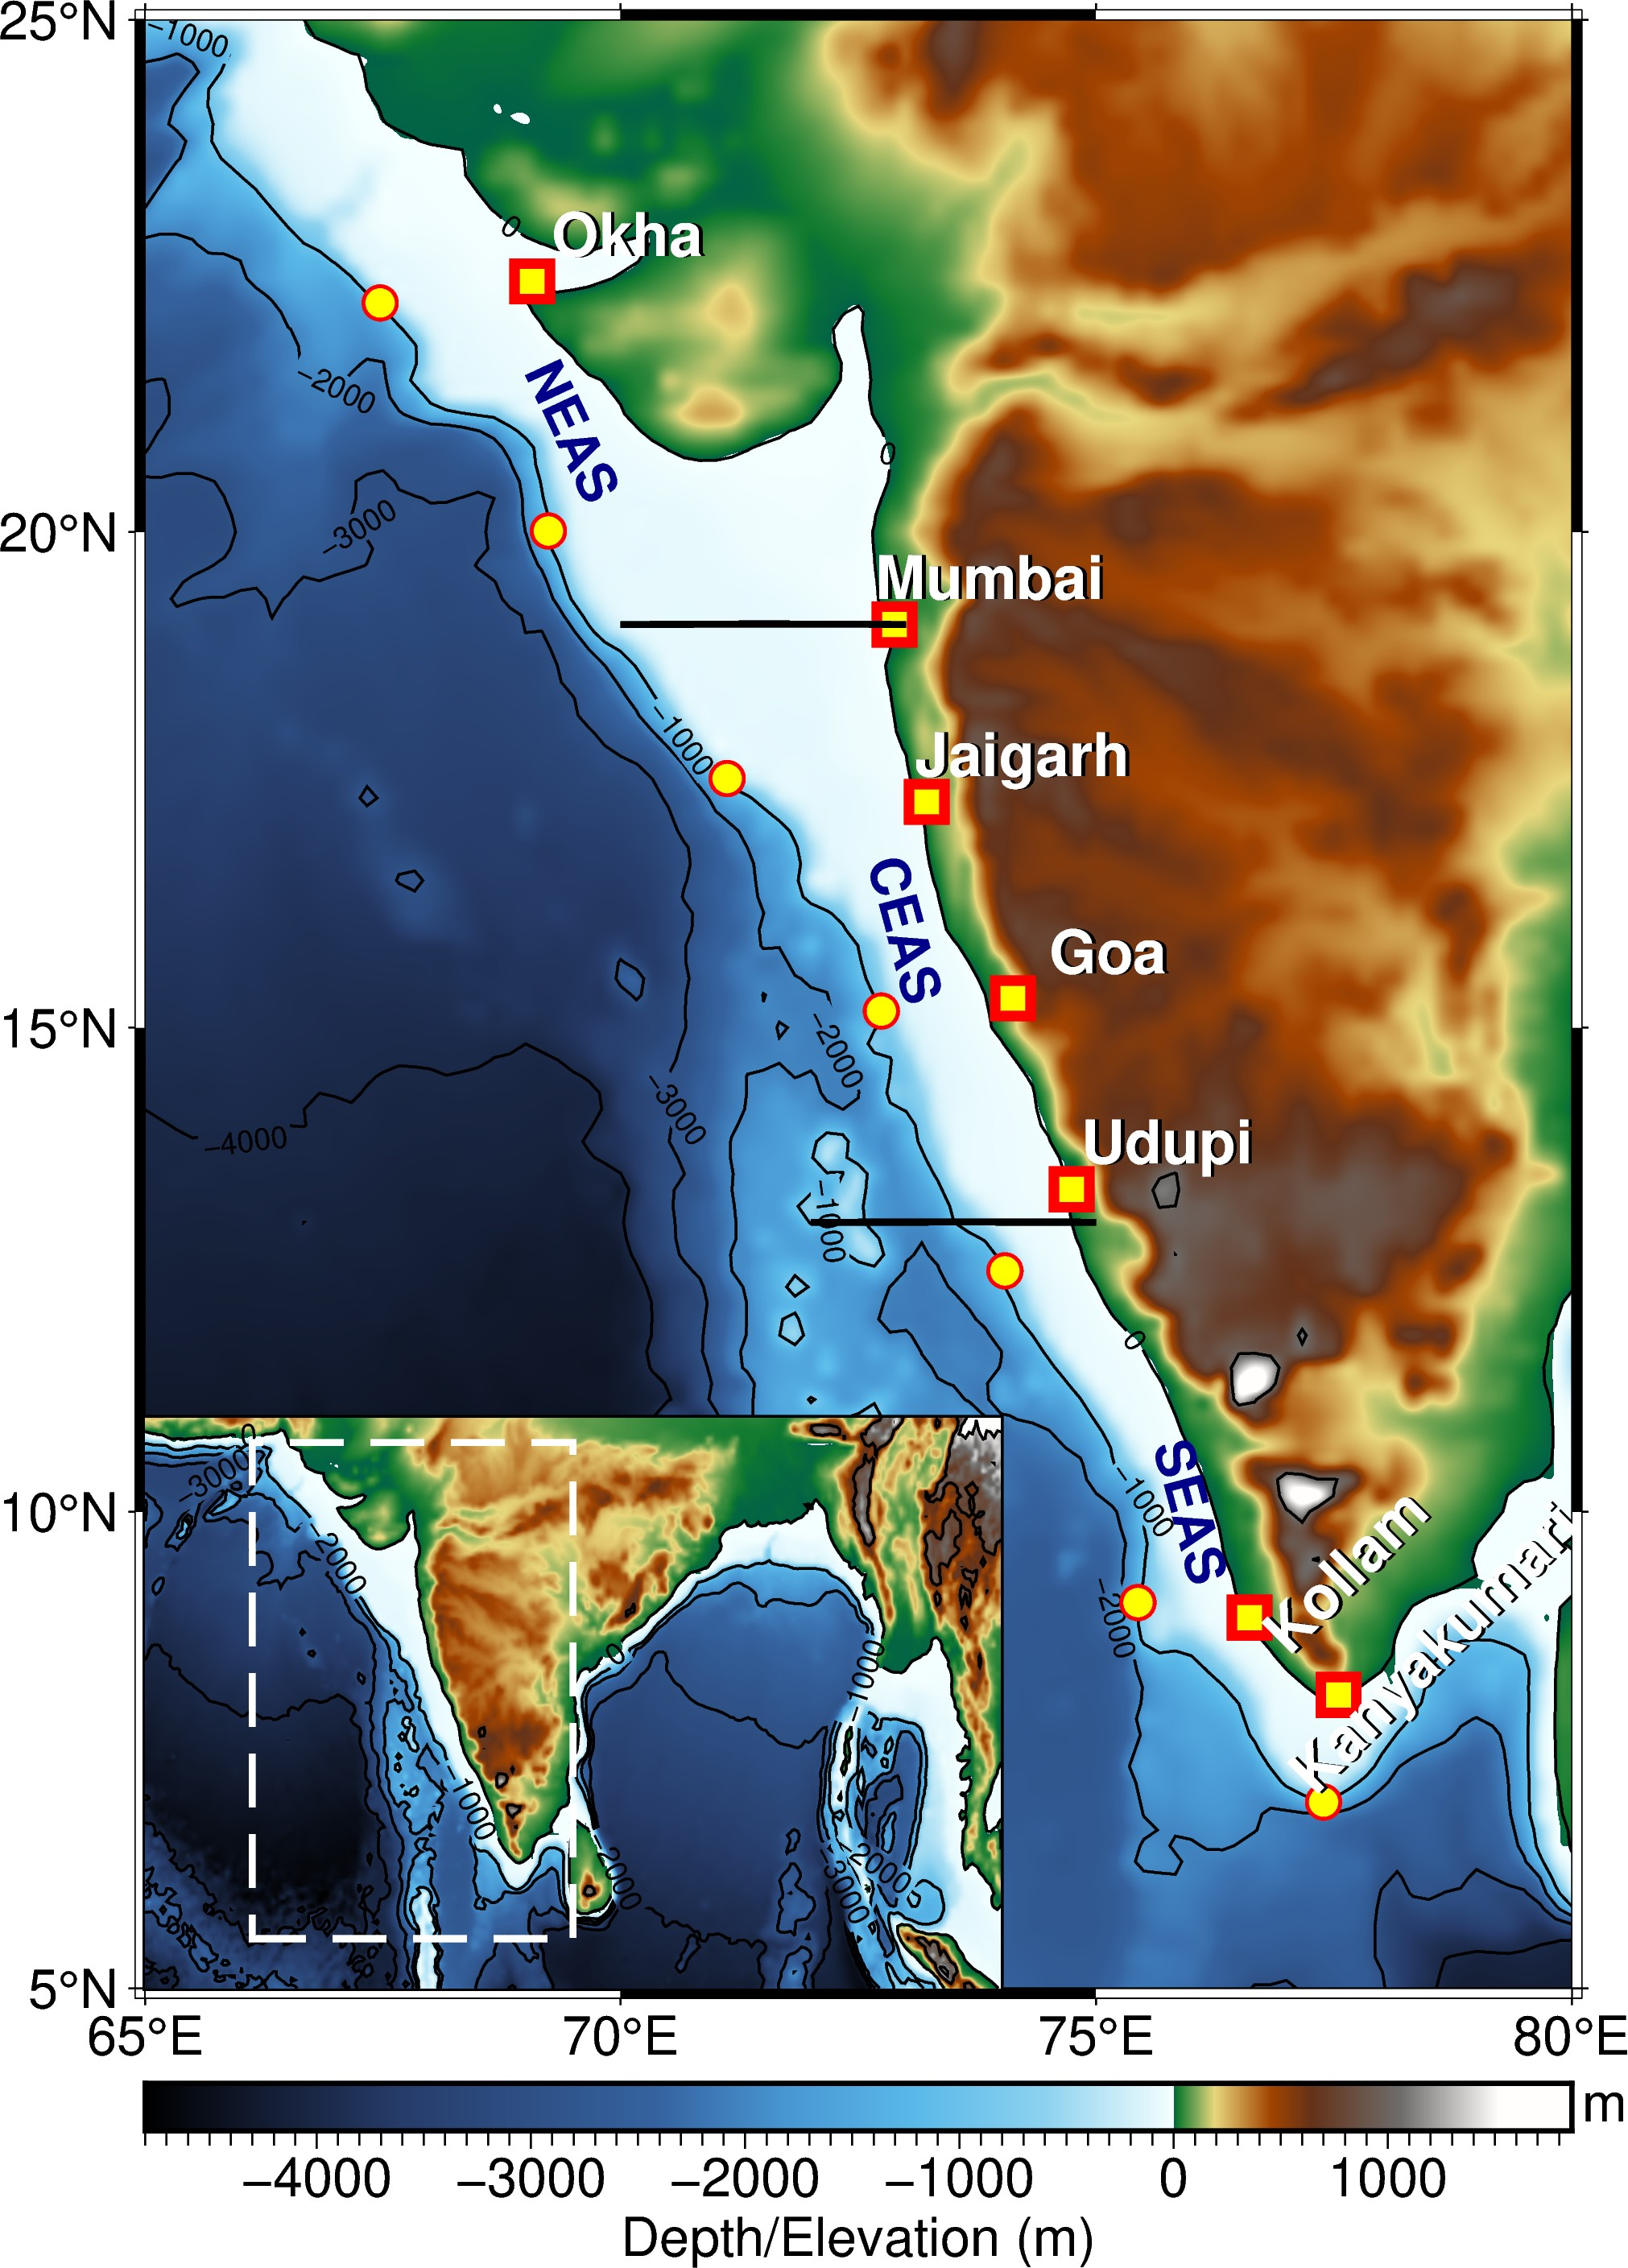
\includegraphics[width=0.6\textwidth]{/media/scilab/disk_ranjan/works/backscatter_wc/figures/adcp_moorings_new1.jpg} 
	\captionsetup{justification=justified,font=footnotesize,skip=0.05\baselineskip,width=0.8\textwidth}
	\caption{Map showing region of interest in eastern Arabian Sea. The slope moorings are
		deployed at $\sim$ 1000 m depth as shown in the bathymetry contour. Note the increase in shelf width as we go poleward along the coast. The mooring sites off Okha and Mumbai are in Northern EAS; Jaigarh and Goa in Central EAS while Kollam and Kanyakumari are at Southern EAS. Udupi is situated at the transition zone of Central and Southern EAS.}
	\label{fig:map}
\end{figure}

\newpage
\begin{figure}[htbp]
	\centering
	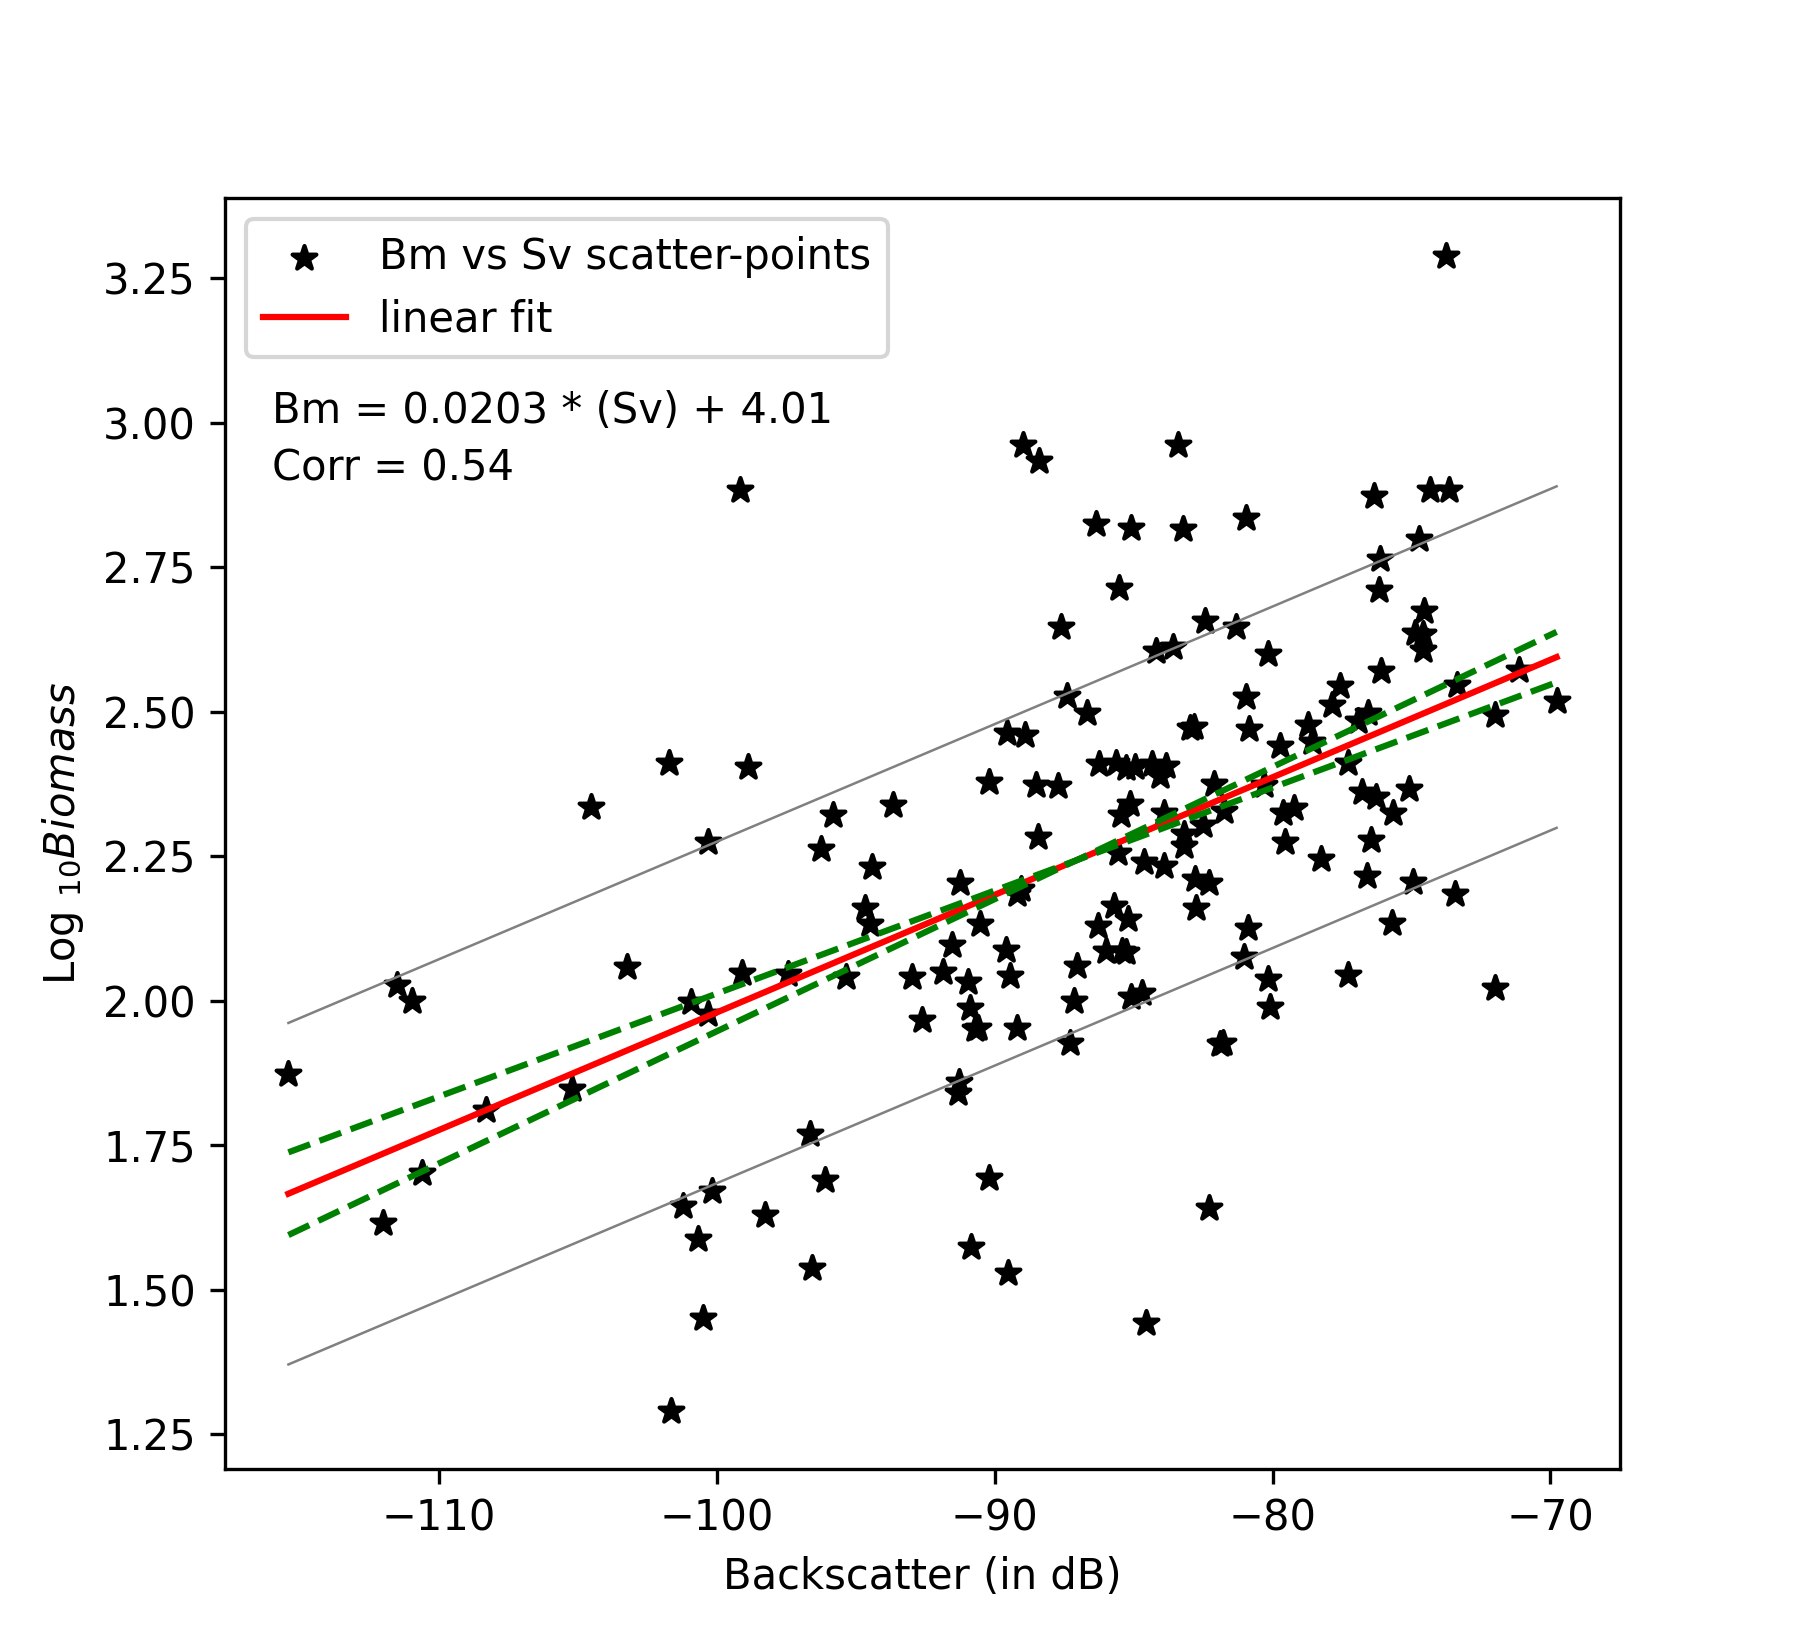
\includegraphics[width=0.5\textwidth]{/media/scilab/disk_ranjan/works/backscatter_wc/figures/backscatter_vs_biomass.png} 
	\captionsetup{justification=justified,font=footnotesize,skip=0.05\baselineskip,width=0.8\textwidth}
	\caption{The linear fit line of Biomass (log$_{10}$ scale) and backscattering strength (in dB). The linear fit line is within the error range of previous result of \citep{aparna2022seasonal} (contained 67 data points) onto which latest zooplankton volumetric sample data (159 data points) is appended. The regression equation is $y\ = (0.02 \pm\ 0.0025) \ x + (4.0144 \pm \ 0.2198) $ and correlation value of 0.54. The dashed green lines denote error range of plausible slope and intercept. The first standard deviation of log$_{10}$(Biomass) is $\pm$ 0.49, which results in the backscatter range of 48.58 dB encompassing the entire backscatter range. It signifies the robustness of zooplankton biomass dependency on ADCP measured backscattering strength.}
	\label{fig:bstobm}
\end{figure}


\newpage

\begin{figure}[htbp]
	\centering
	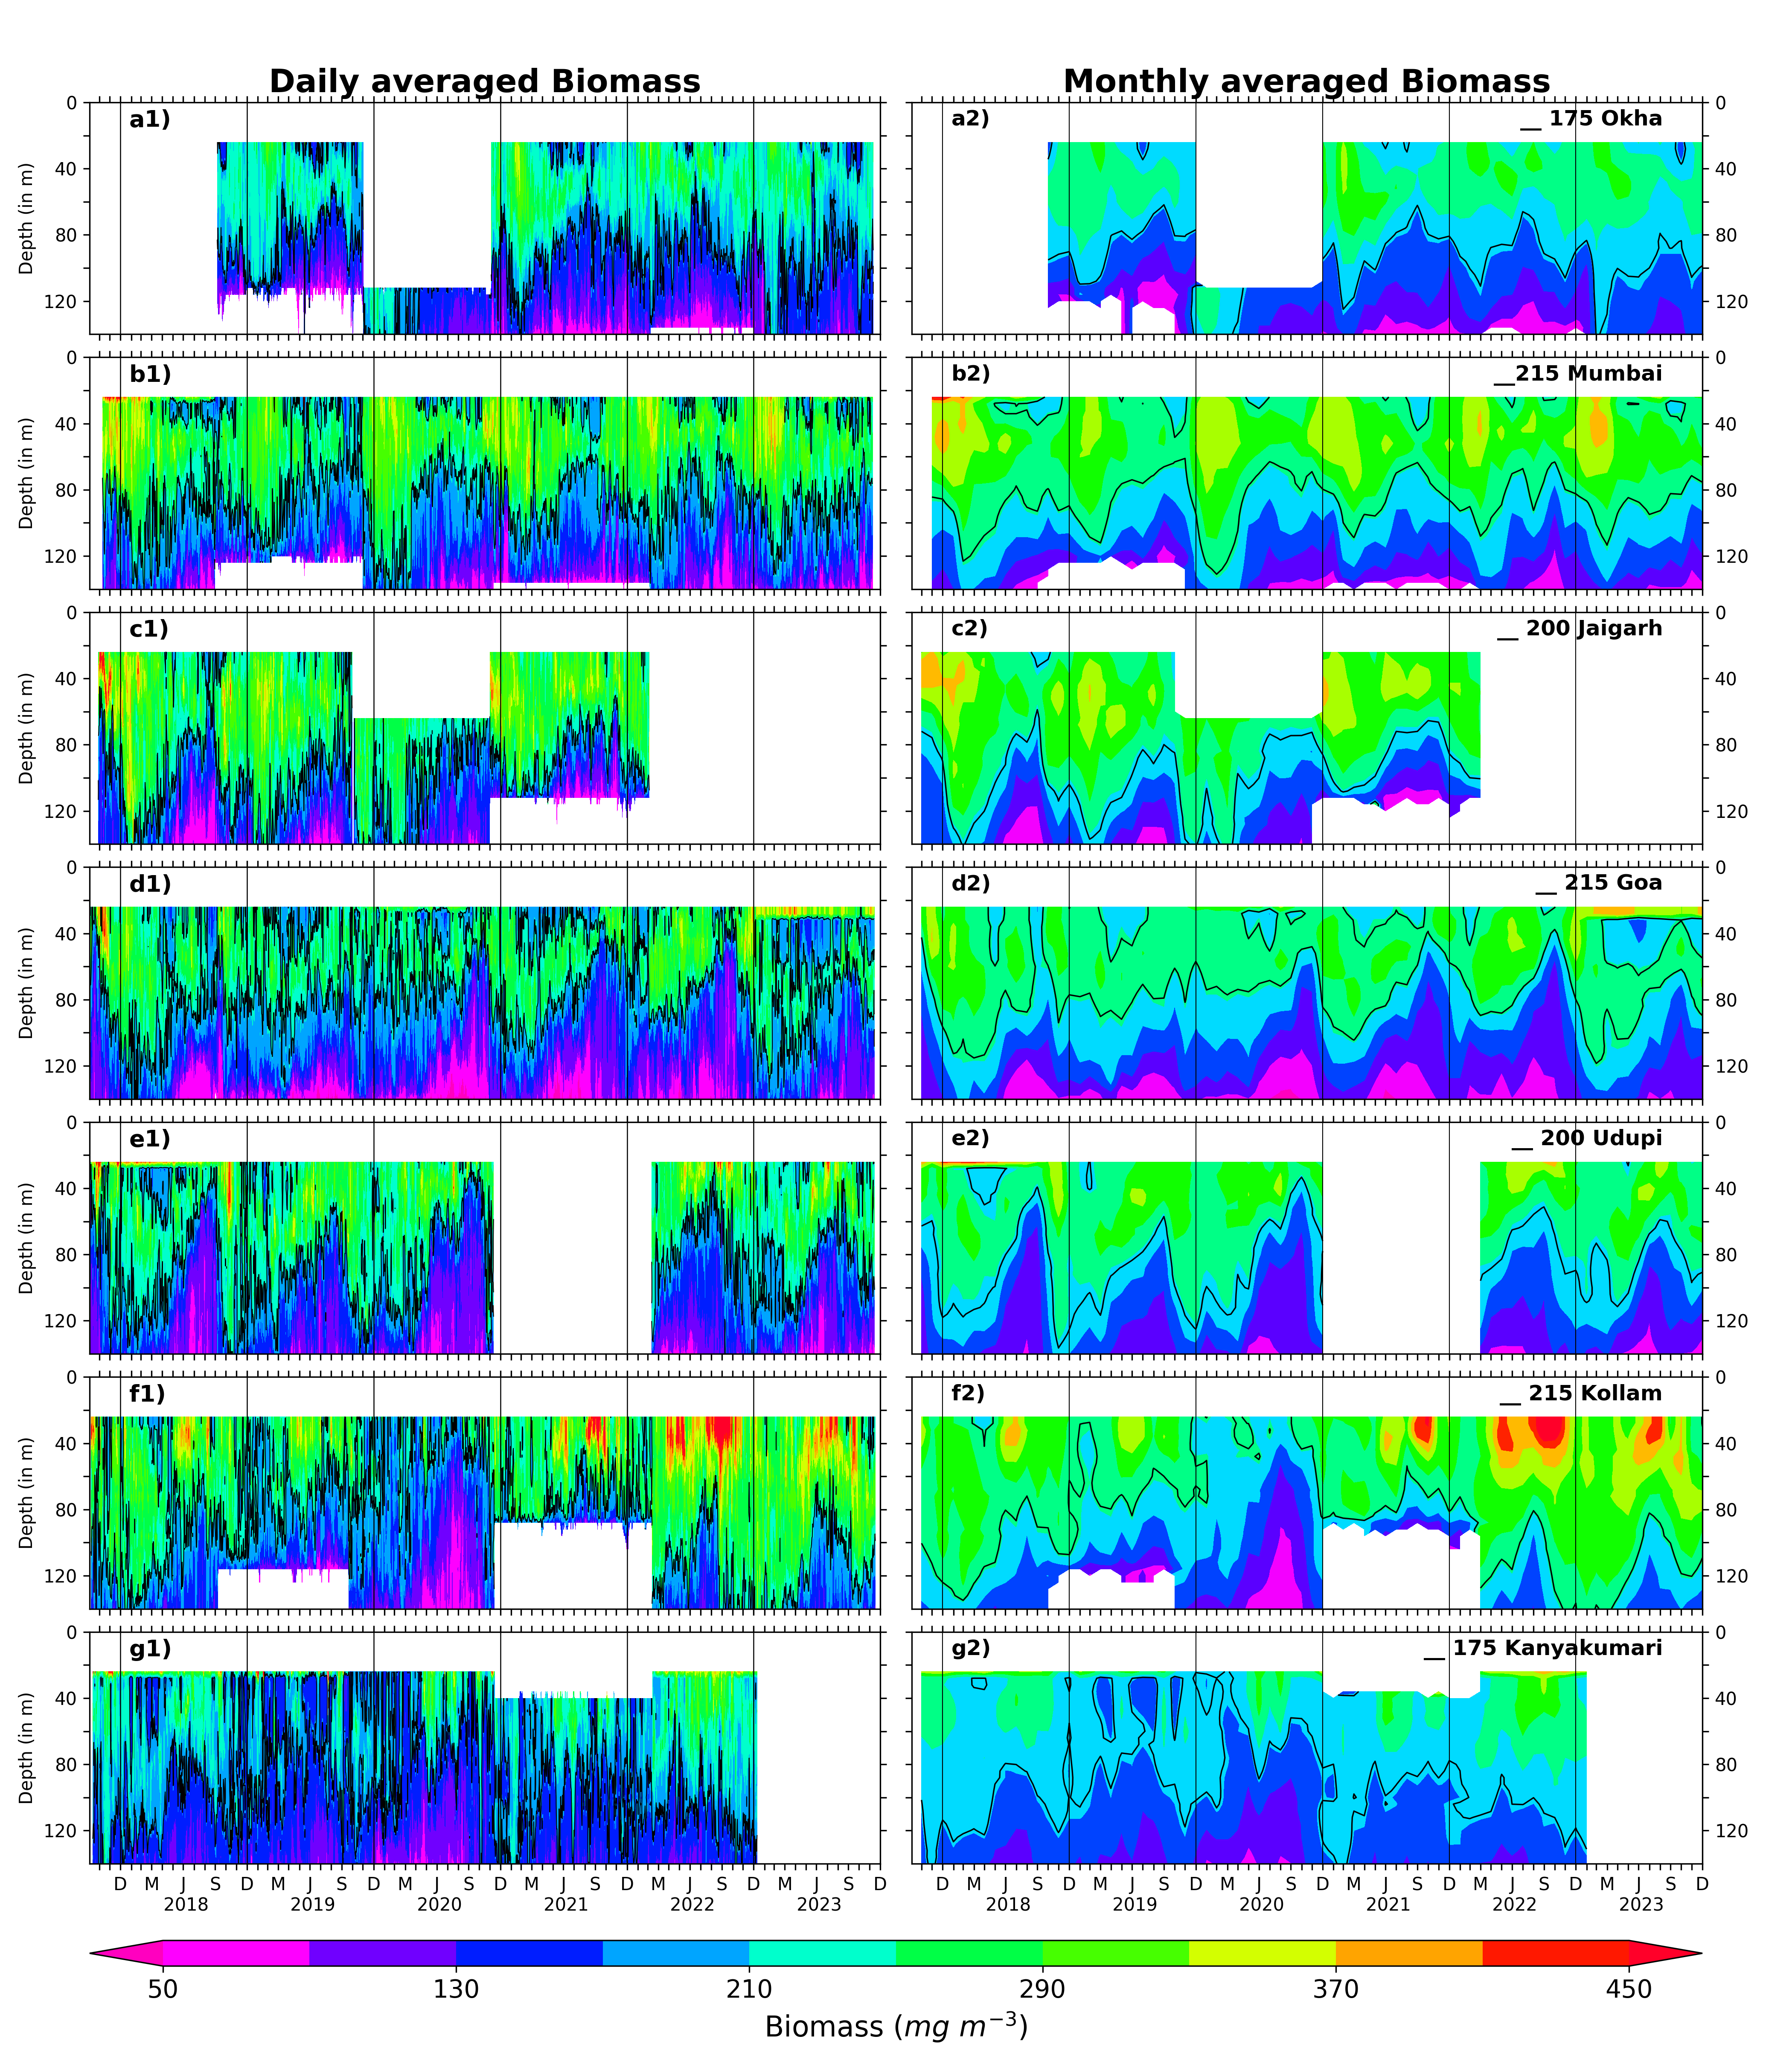
\includegraphics[width=\textwidth]{/media/scilab/disk_ranjan/works/backscatter_wc/figures/biomass_daily_monthly.png} 
	\captionsetup{justification=justified,font=footnotesize,skip=0.05\baselineskip,width=\textwidth}
	\caption{The Daily and monthly averaged biomass for EAS moorings, north (top) to south (bottom). The black contours are marking of 175 $mg\ m^{-3}$ biomass for Okha and Kanyakumari; 215 $mg\ m^{-3}$  for Mumbai, Goa and Kollam. The biomass contours are distinct and different based on the physico-chemical parameters and the one that best explains seasonality at respective location.  The top 10 \% of data is discarded due to echo noise. The dashed line at 22 m marks the top-depth of first bin i.e, 24 m.}
	\label{fig:dailynmonthly}
\end{figure}

\begin{figure}[htbp]
	\centering
	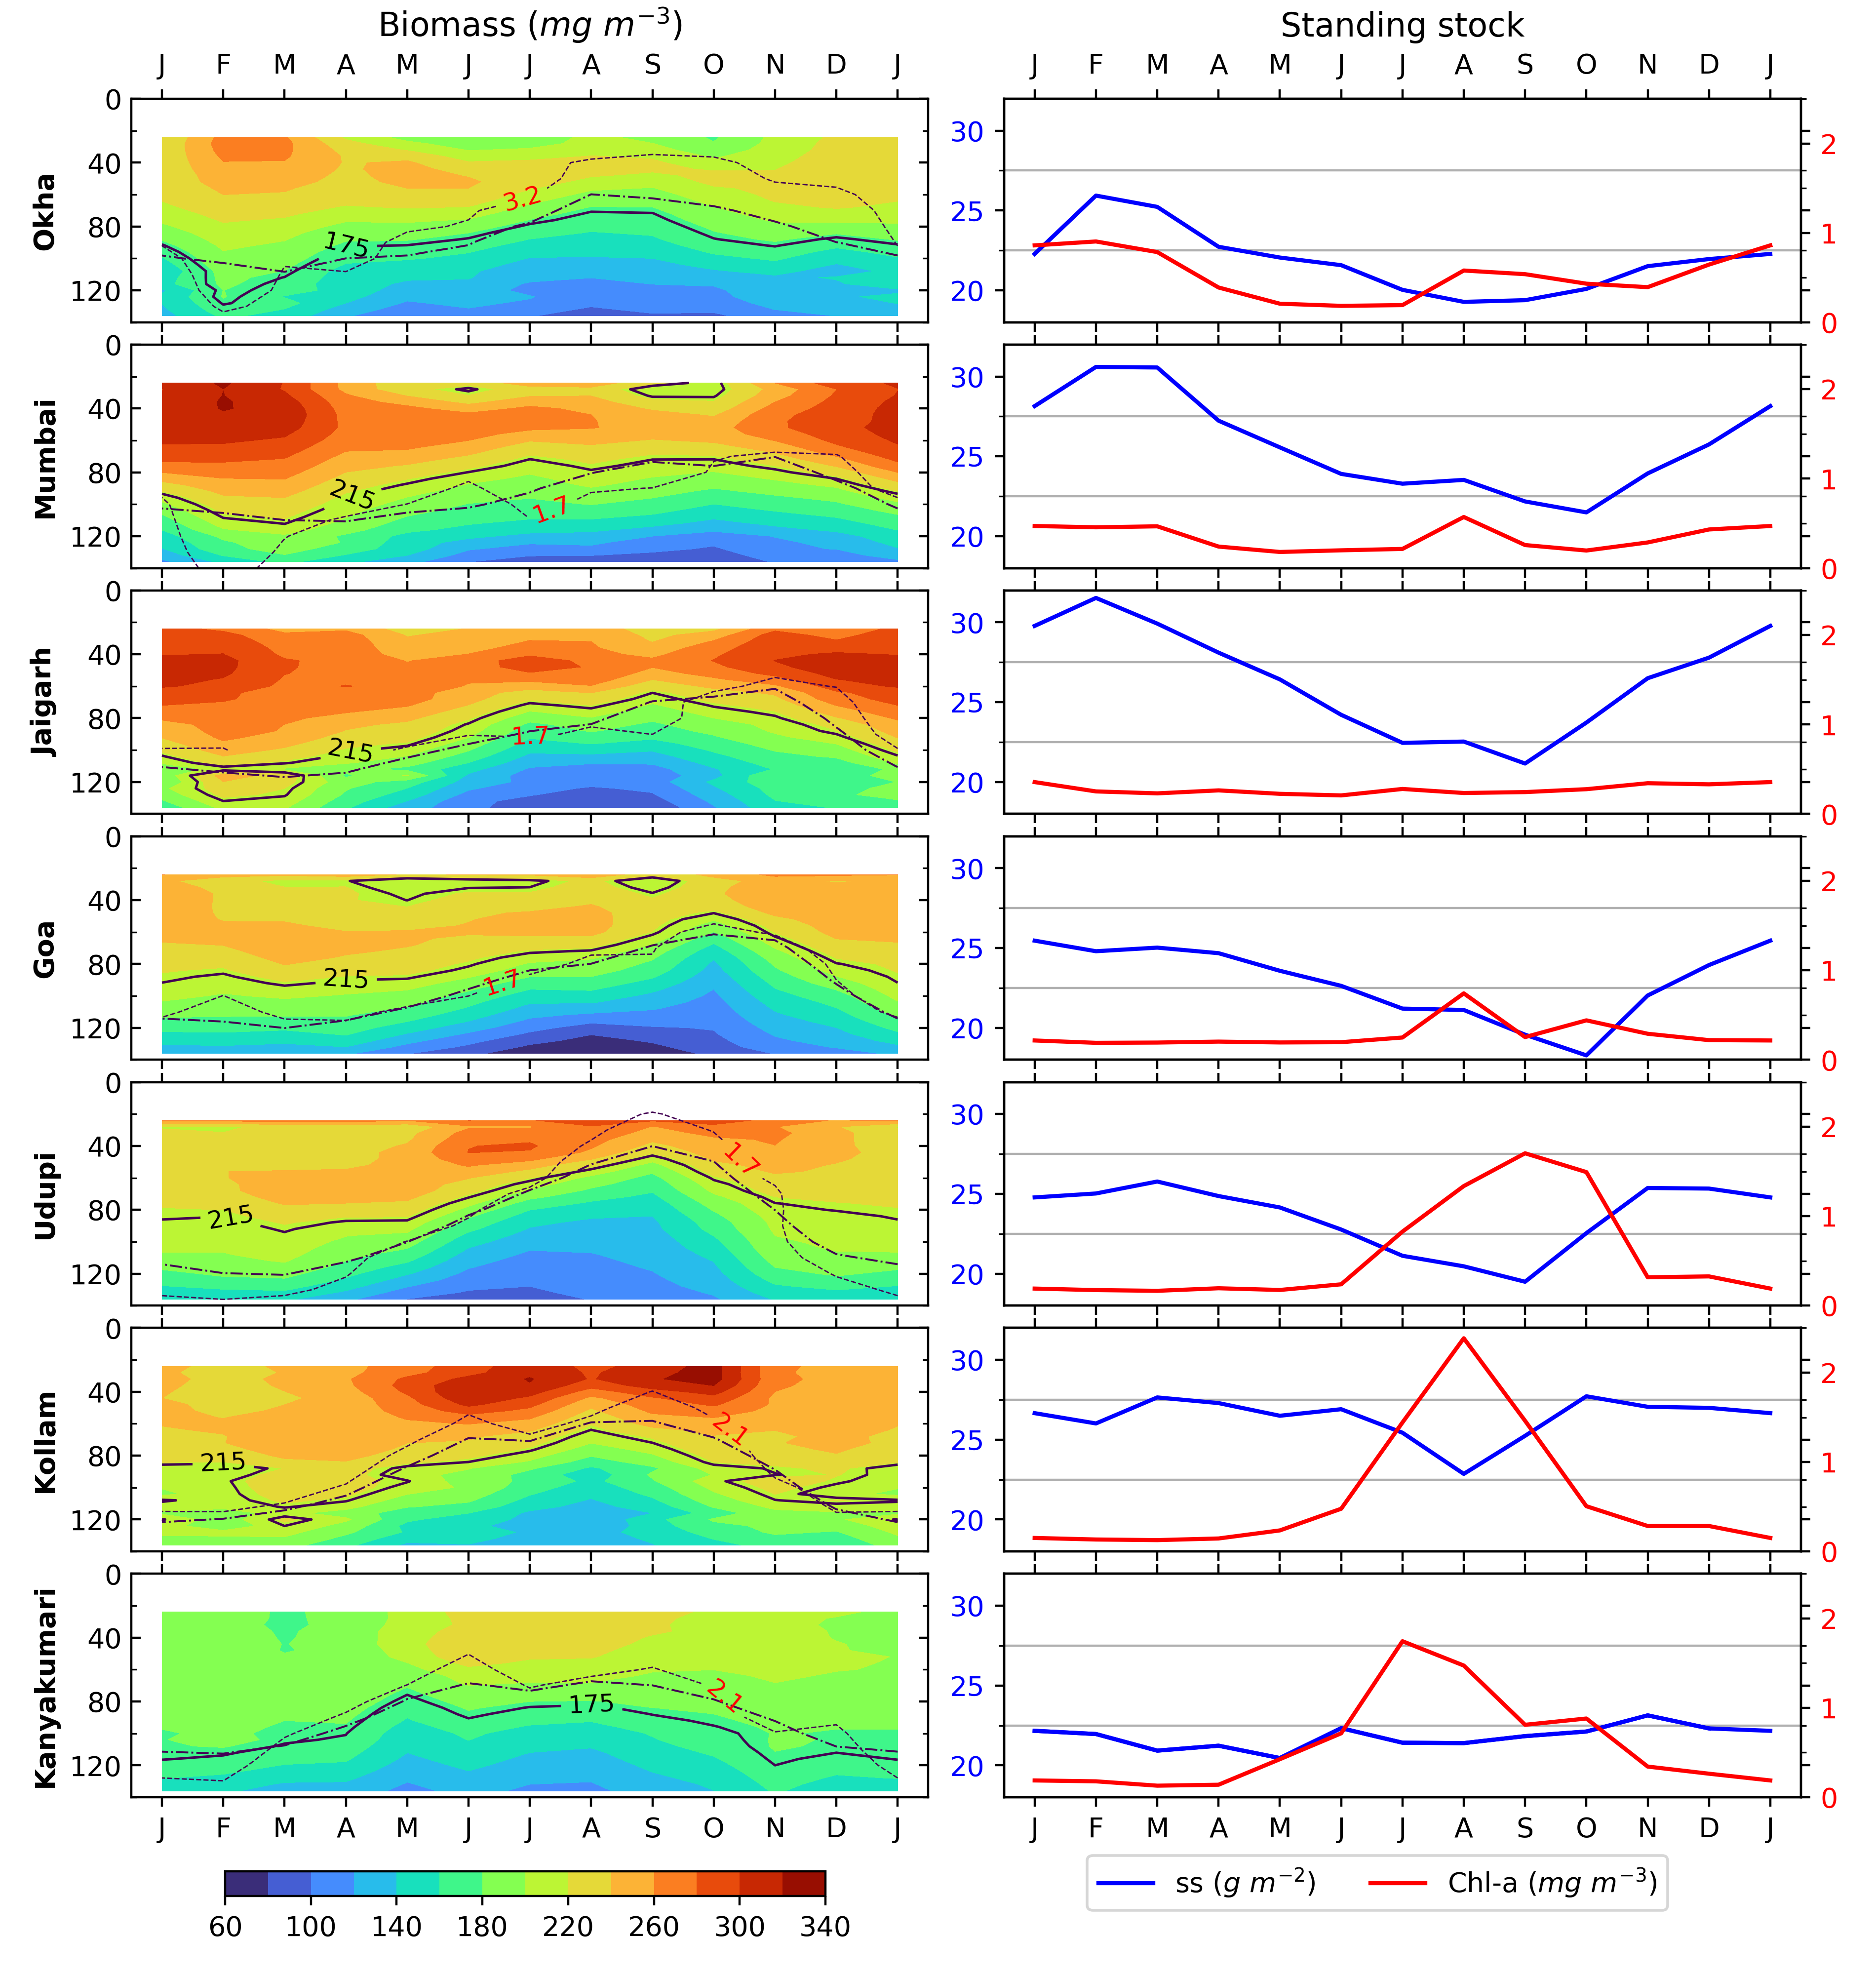
\includegraphics[width=\textwidth]{/media/scilab/disk_ranjan/works/backscatter_wc/figures/climatology_biomass_ss_chl.png} 
	\captionsetup{justification=justified,font=footnotesize,skip=0.05\baselineskip,width=\textwidth}
	\caption{Monthly climatology of zooplankton biomass is shown in left panels for 7 locations, (top to bottom is southward). The D175 \& D215 are shown in solid lines; dashed line represents the depth of 23 C isotherm; oxygen contours are shown in dotted lines and labeled for each mooring. The right set of panel plots is showing ZSS and chlorophyll climatology for corresponding locations.}
	\label{fig:zsschlclim}
\end{figure}

\begin{figure}[htbp]
	\centering
	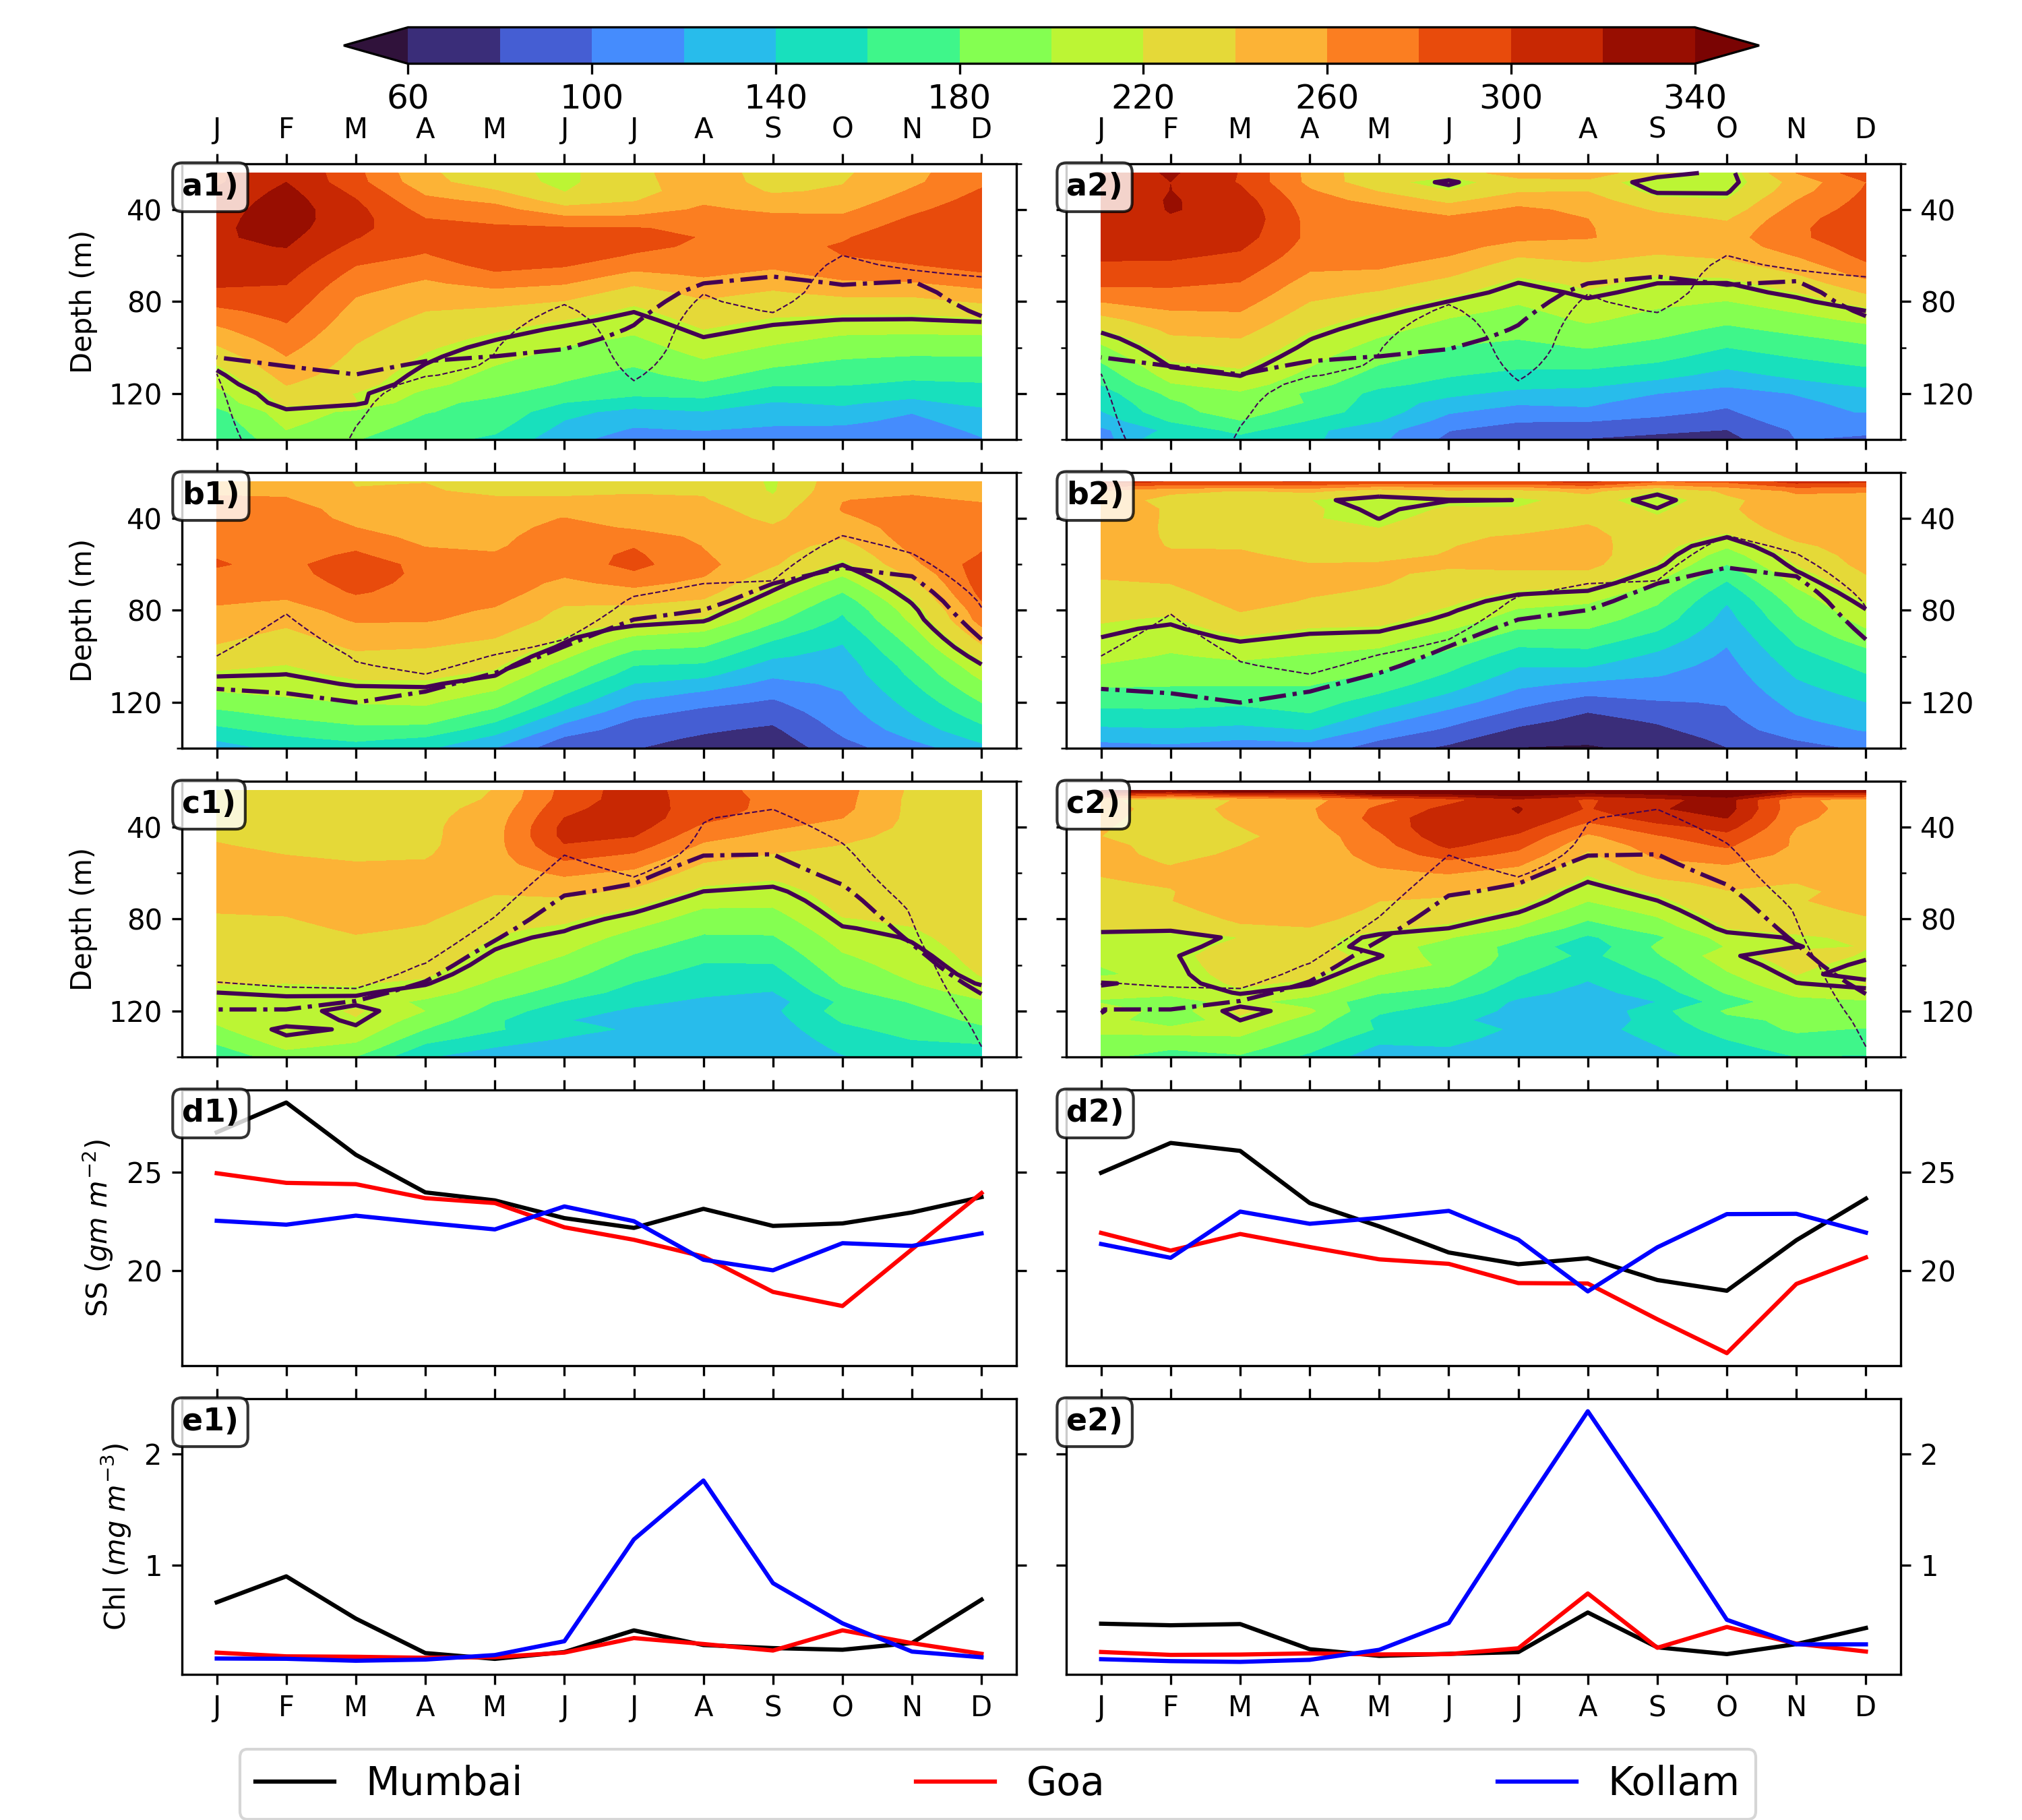
\includegraphics[width=\textwidth]{/media/scilab/disk_ranjan/works/backscatter_wc/figures/aparna_ranjan_climatology_comparison.png} 
	\captionsetup{justification=justified,font=footnotesize,skip=0.05\baselineskip,width=\textwidth}
	\caption{Monthly climatology of zooplankton biomass is shown in left panels for 3 locations which were earlier used in \citep{aparna2022seasonal}; a1, b1 \& c1 is the biomass climatology for Mumbai, Goa and Kollam, d1 is for ZSS climatology, e1 is for chlorophyll biomass climatology; a2, b2, c2, d2 \& e2 is same but based on data from 2017 to 2023. The D215 is shown in solid line. The dashed line represents the depth of 23 $^o$C isotherm; oxygen contours are shown in dotted lines and labeled for each mooring.}
	\label{fig:zsschlclimcomp}
\end{figure}

\begin{figure}[htbp]
	\centering
	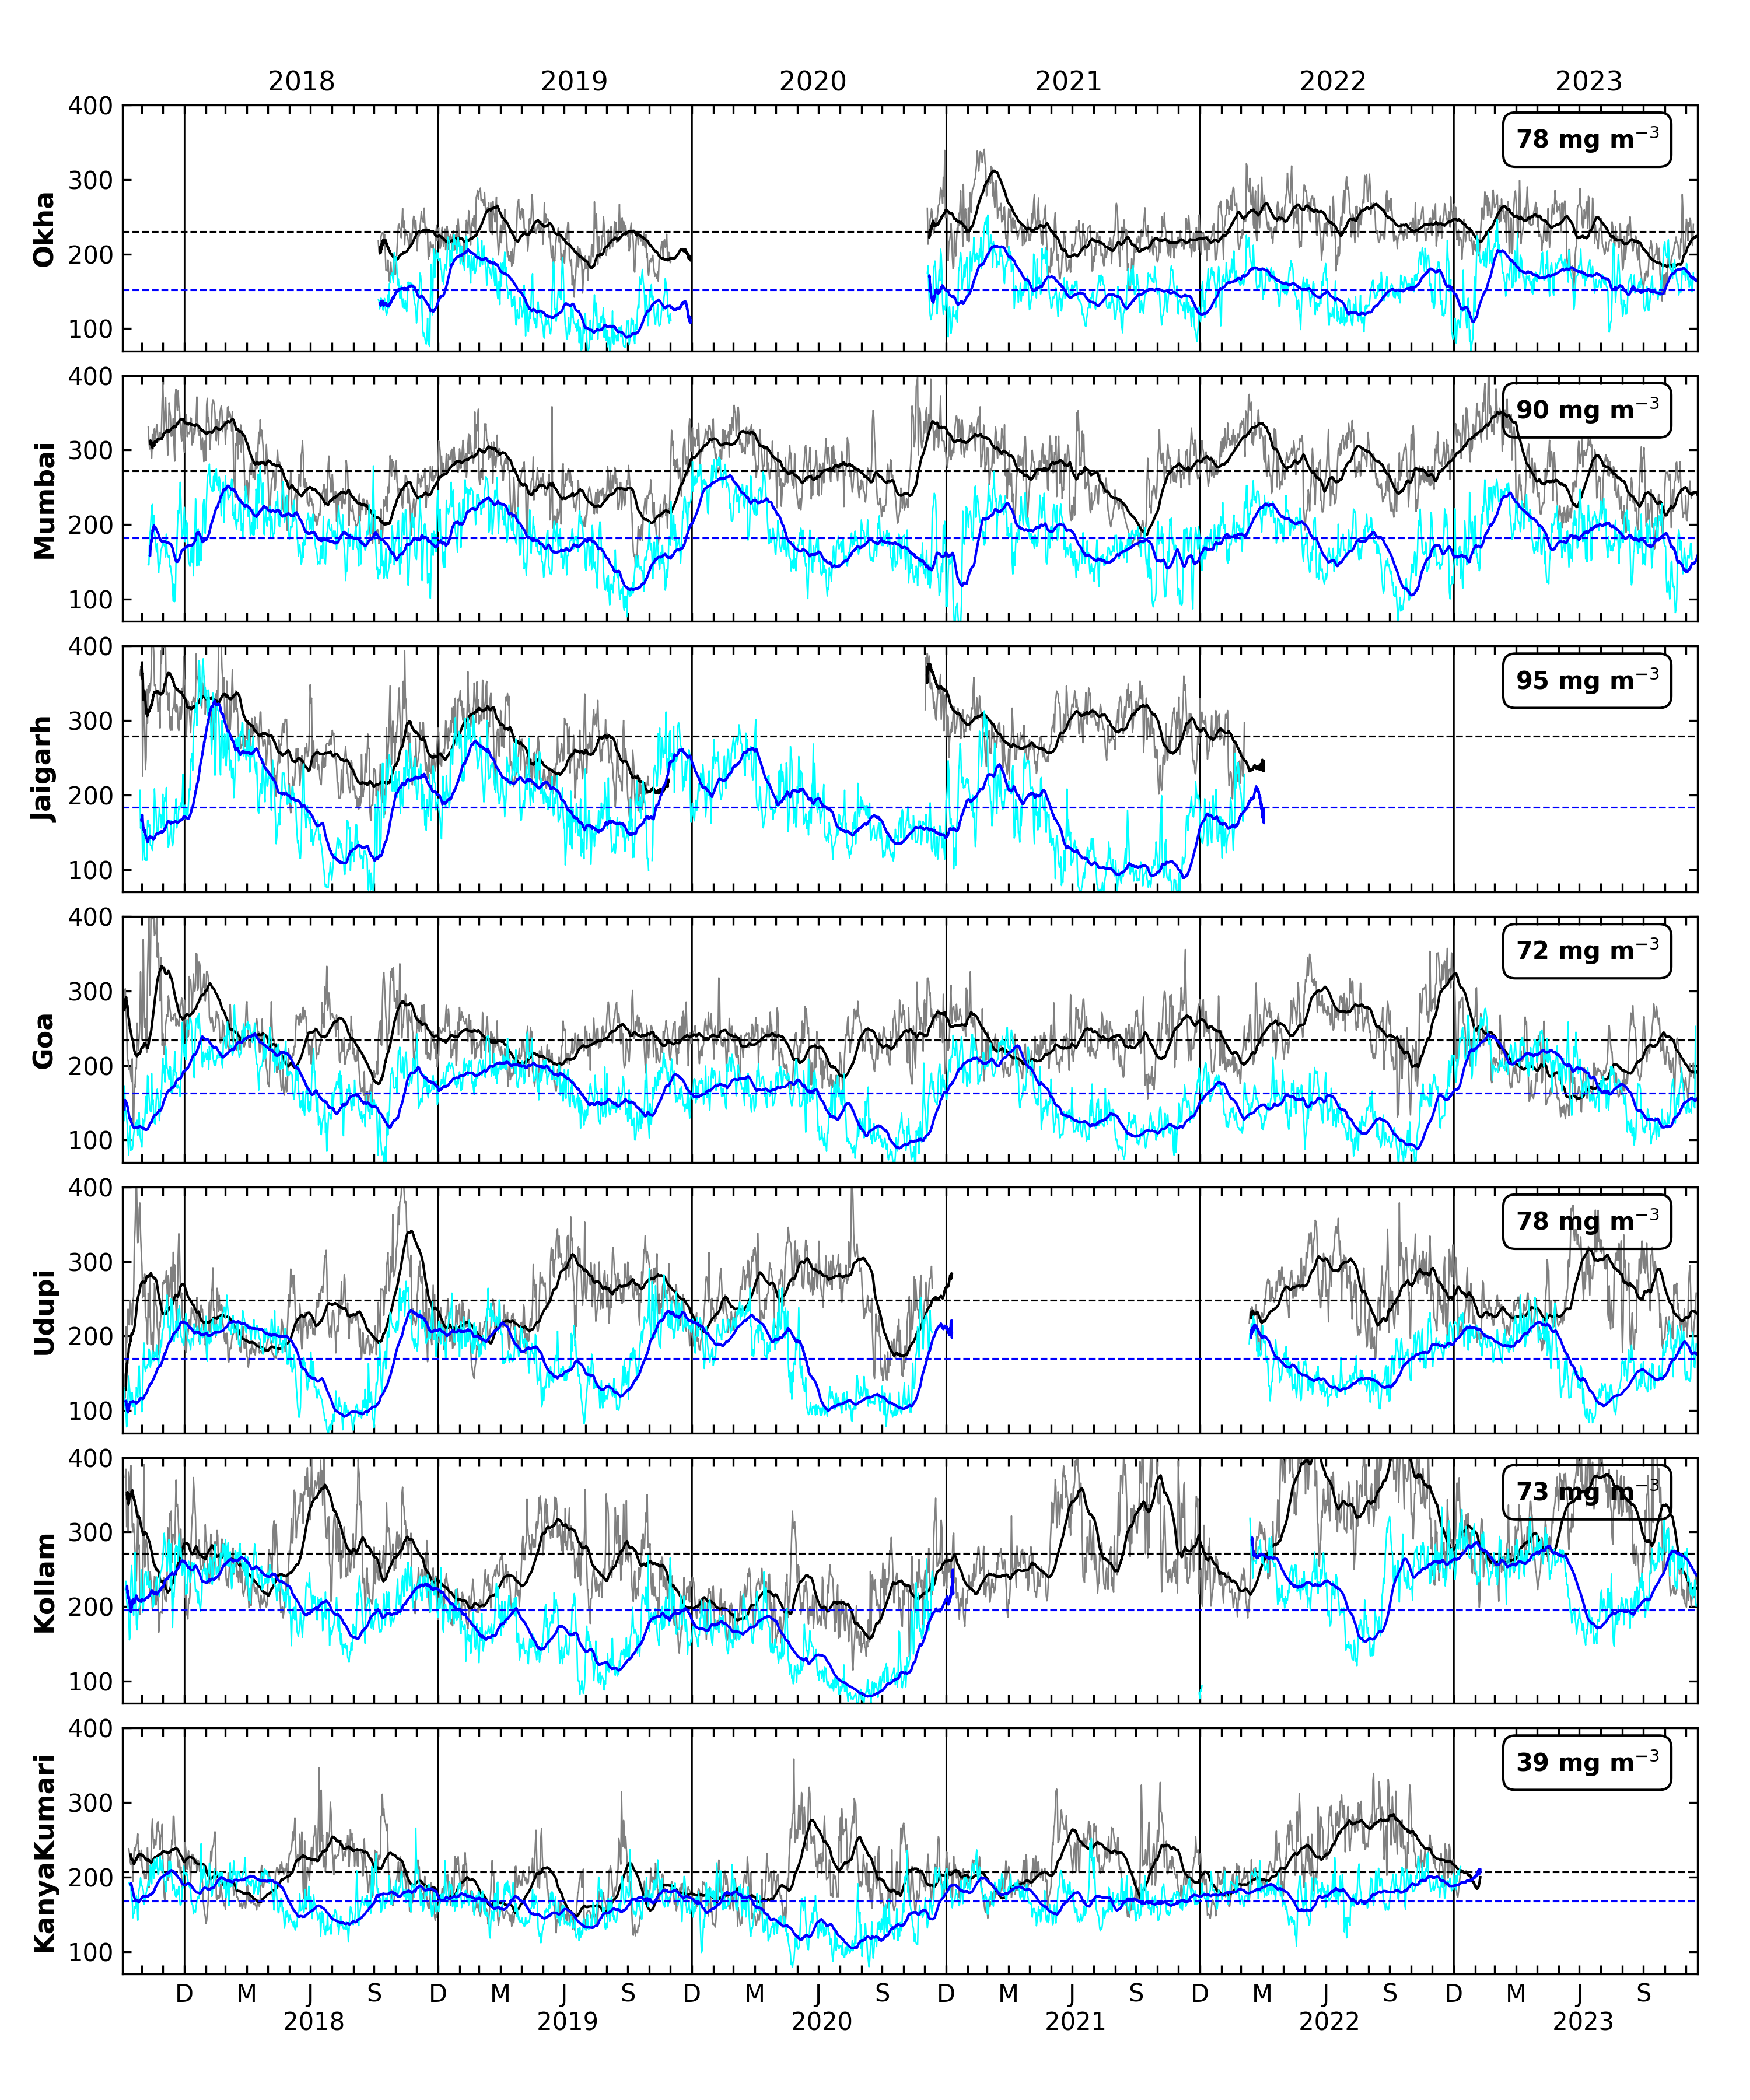
\includegraphics[width=\textwidth]{/media/scilab/disk_ranjan/works/backscatter_wc/figures/biomass_40m_104m.png} 
	\captionsetup{justification=justified,font=footnotesize,skip=0.05\baselineskip,width=\textwidth}
	\caption{The daily biomass at depth of 40 m and 104 m for all locations shown by grey and cyan curves. The black and blue lines shows the 30 day rolling averaged biomass at 40 and 104 m, respectively. Notice the bursts seen in the daily data ranging from few days to weeks.}
	\label{fig:compfourty}
\end{figure}

\begin{figure}[htbp]
	\centering
	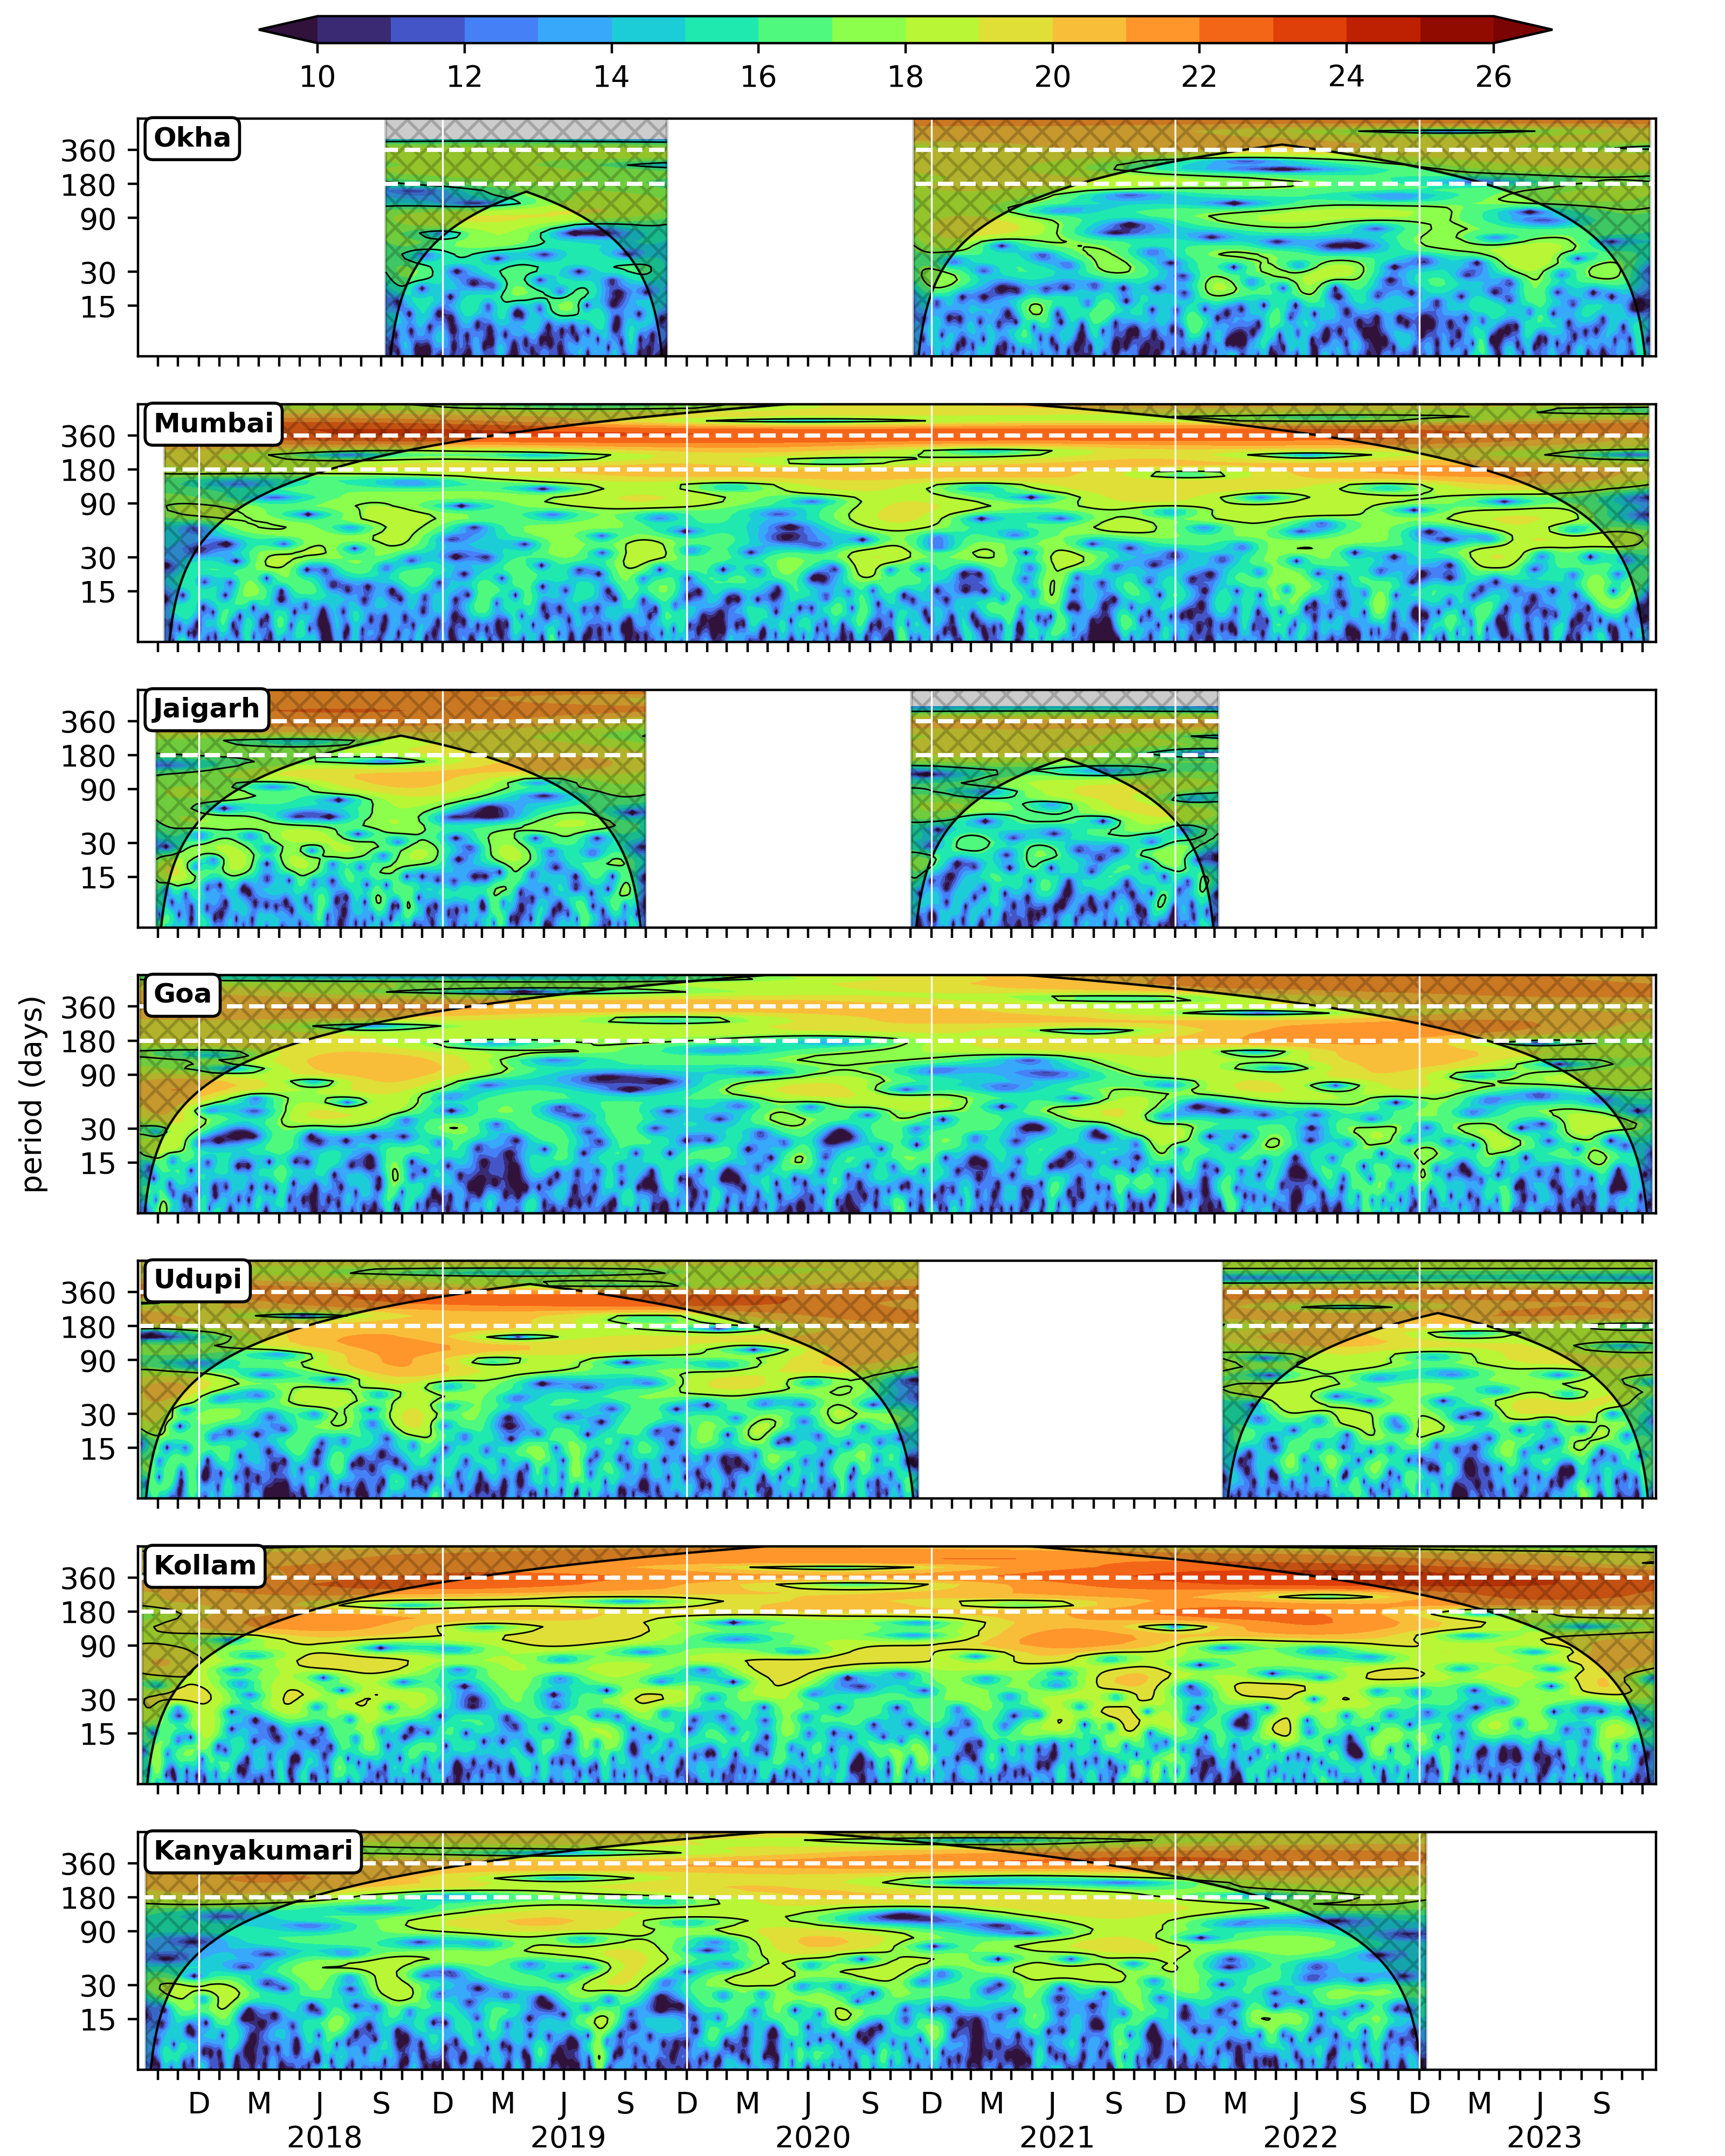
\includegraphics[width=\textwidth]{/media/scilab/disk_ranjan/works/backscatter_wc/figures/west_coast_wavelet_40m_scale.png} 
	\captionsetup{justification=justified,font=footnotesize,skip=0.05\baselineskip,width=\textwidth}
	\caption{Wavelet power spectra (Morlet) of the 40 m zooplankton biomass plotted against time as abscissa and period in days as ordinate. The wavelet power is in log$_2$ scale, the 95 \% significance is marked in black contours; the cross-shaded region falls under cone of influence. Vertical white lines separates years.}
	\label{fig:wavefourty}
\end{figure}

\begin{figure}[htbp]
	\centering
	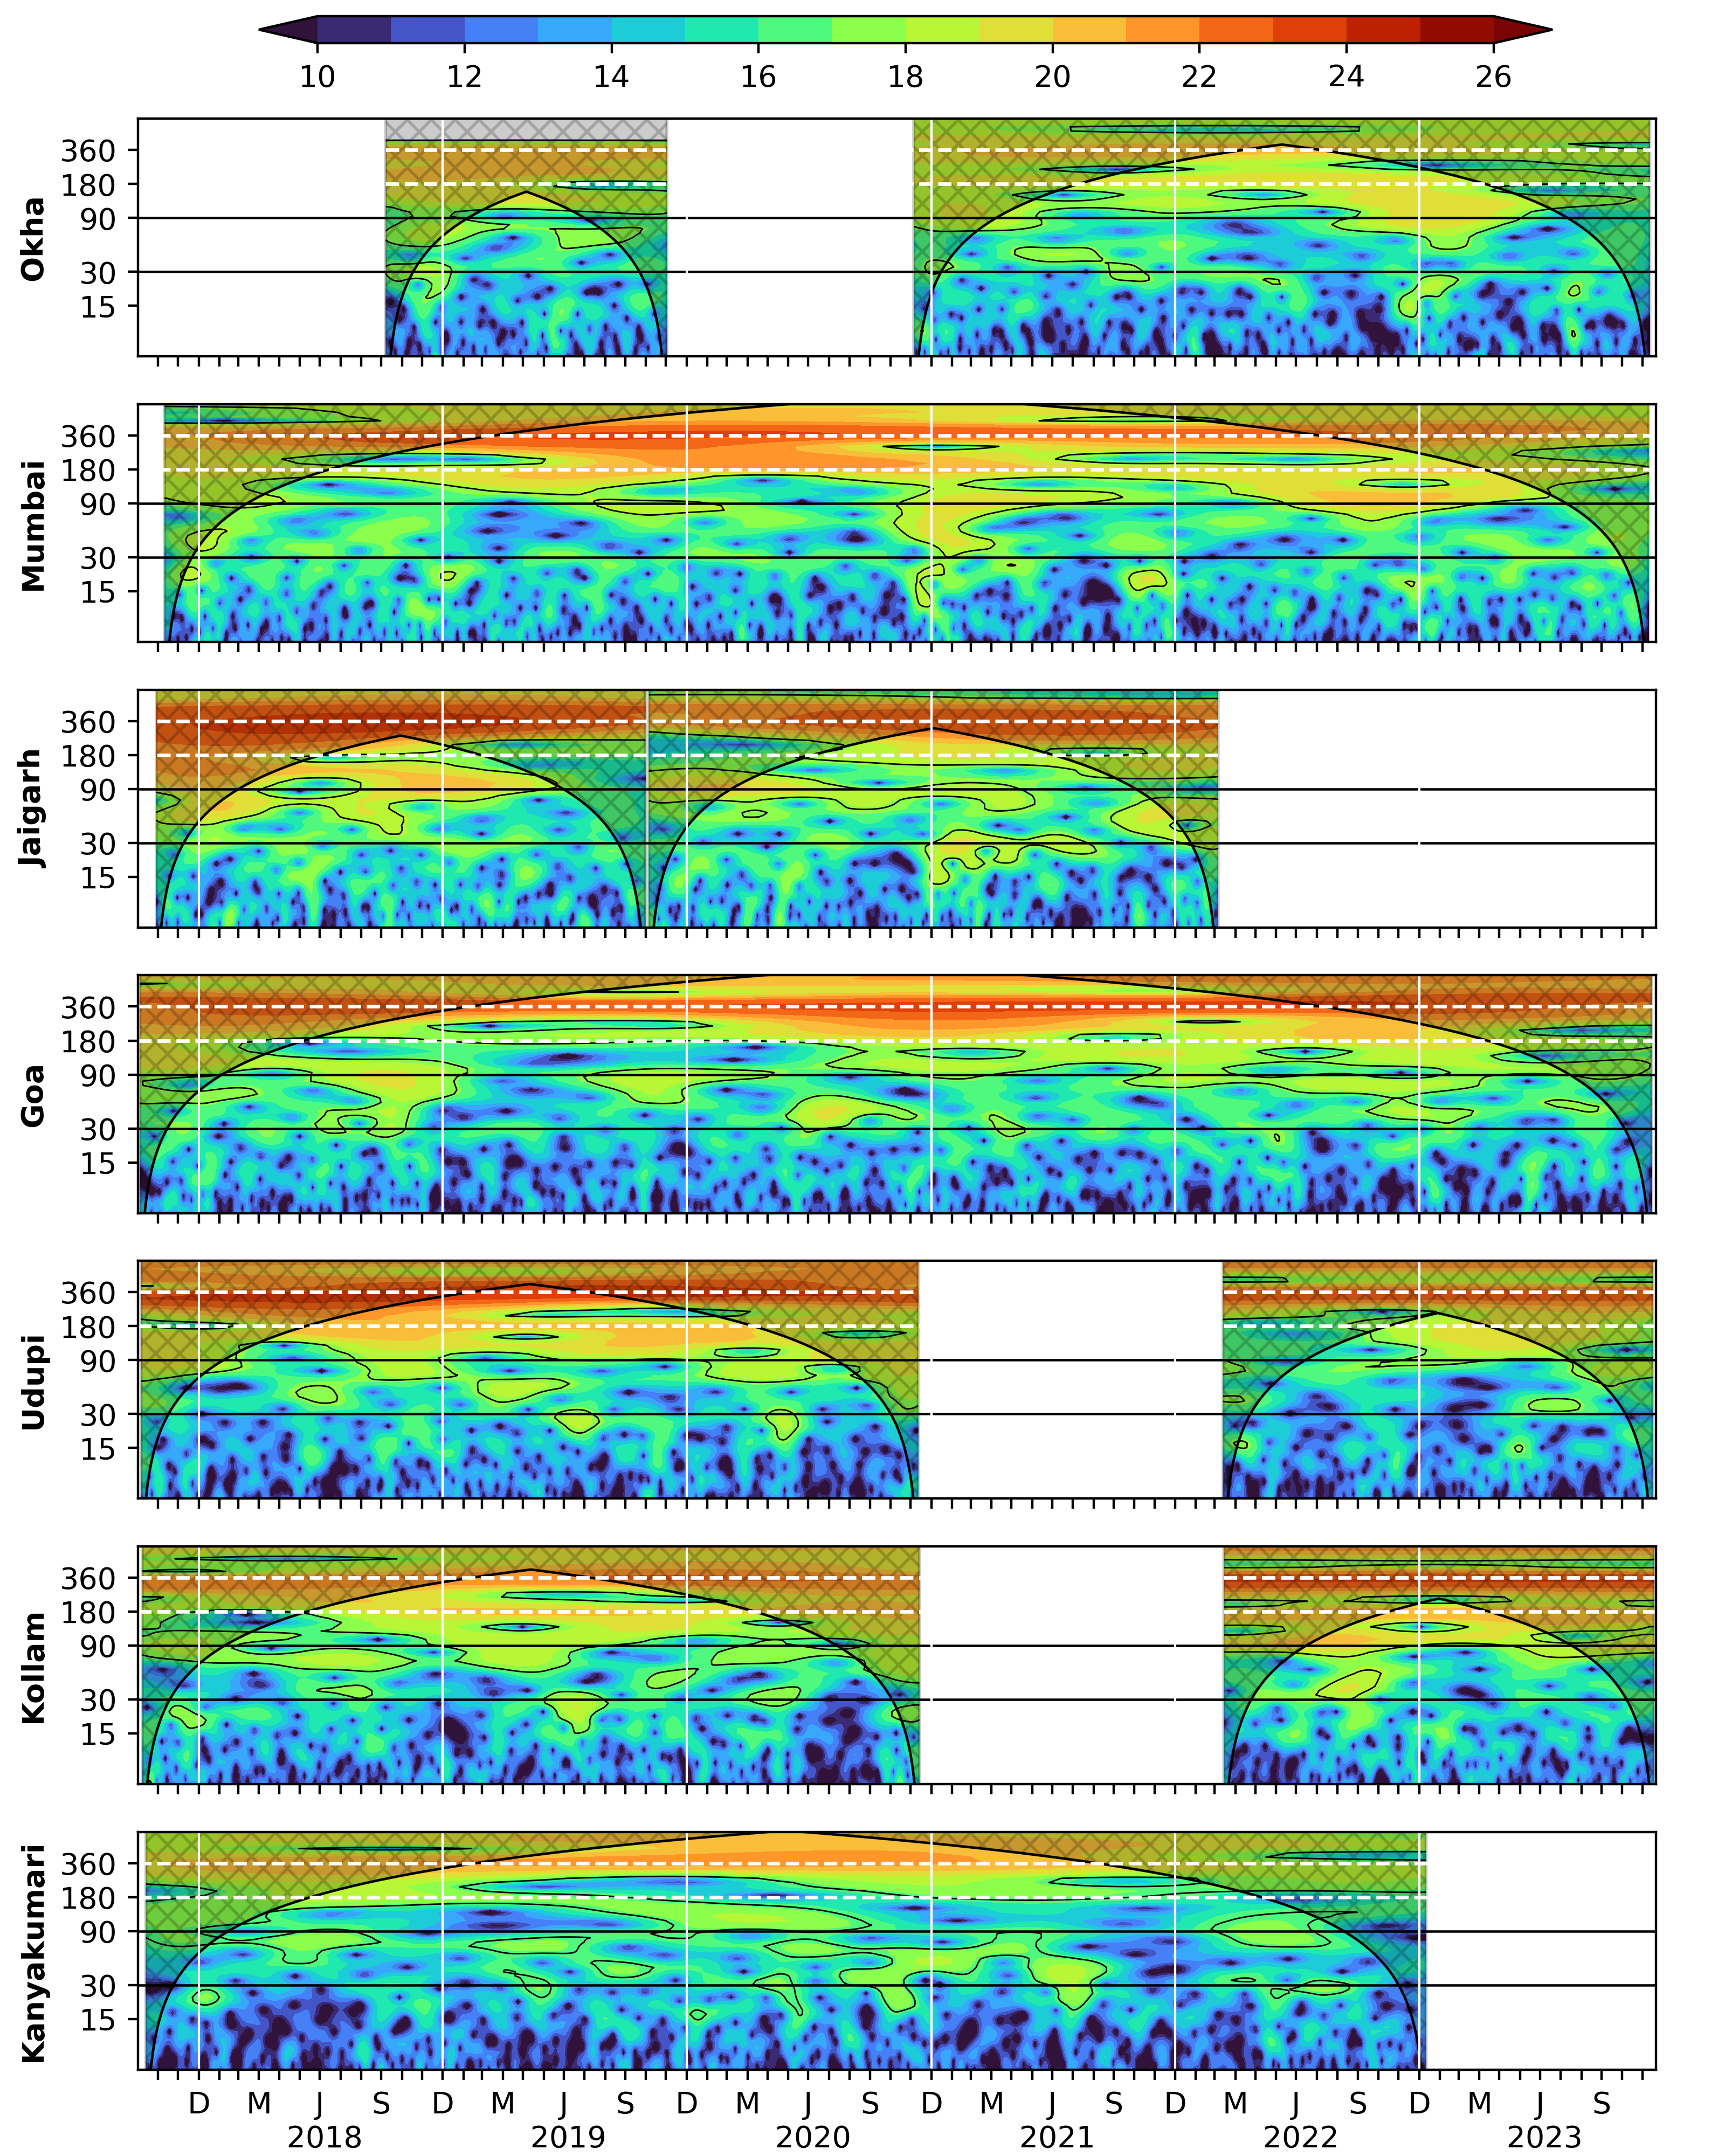
\includegraphics[width=\textwidth]{/media/scilab/disk_ranjan/works/backscatter_wc/figures/west_coast_wavelet_104m_scale.png} 
	\captionsetup{justification=justified,font=footnotesize,skip=0.05\baselineskip,width=\textwidth}
	\caption{Wavelet power spectra (Morlet) of the 104 m zooplankton biomass plotted against time as abscissa and period in days as ordinate. The wavelet power is in log$_2$ scale, the 95 \% significance is marked in black contours; the cross-shaded region falls under cone of influence. The vertical white lines separates years.}
	\label{fig:wave104}
\end{figure}

\begin{figure}[htbp]
	\centering
	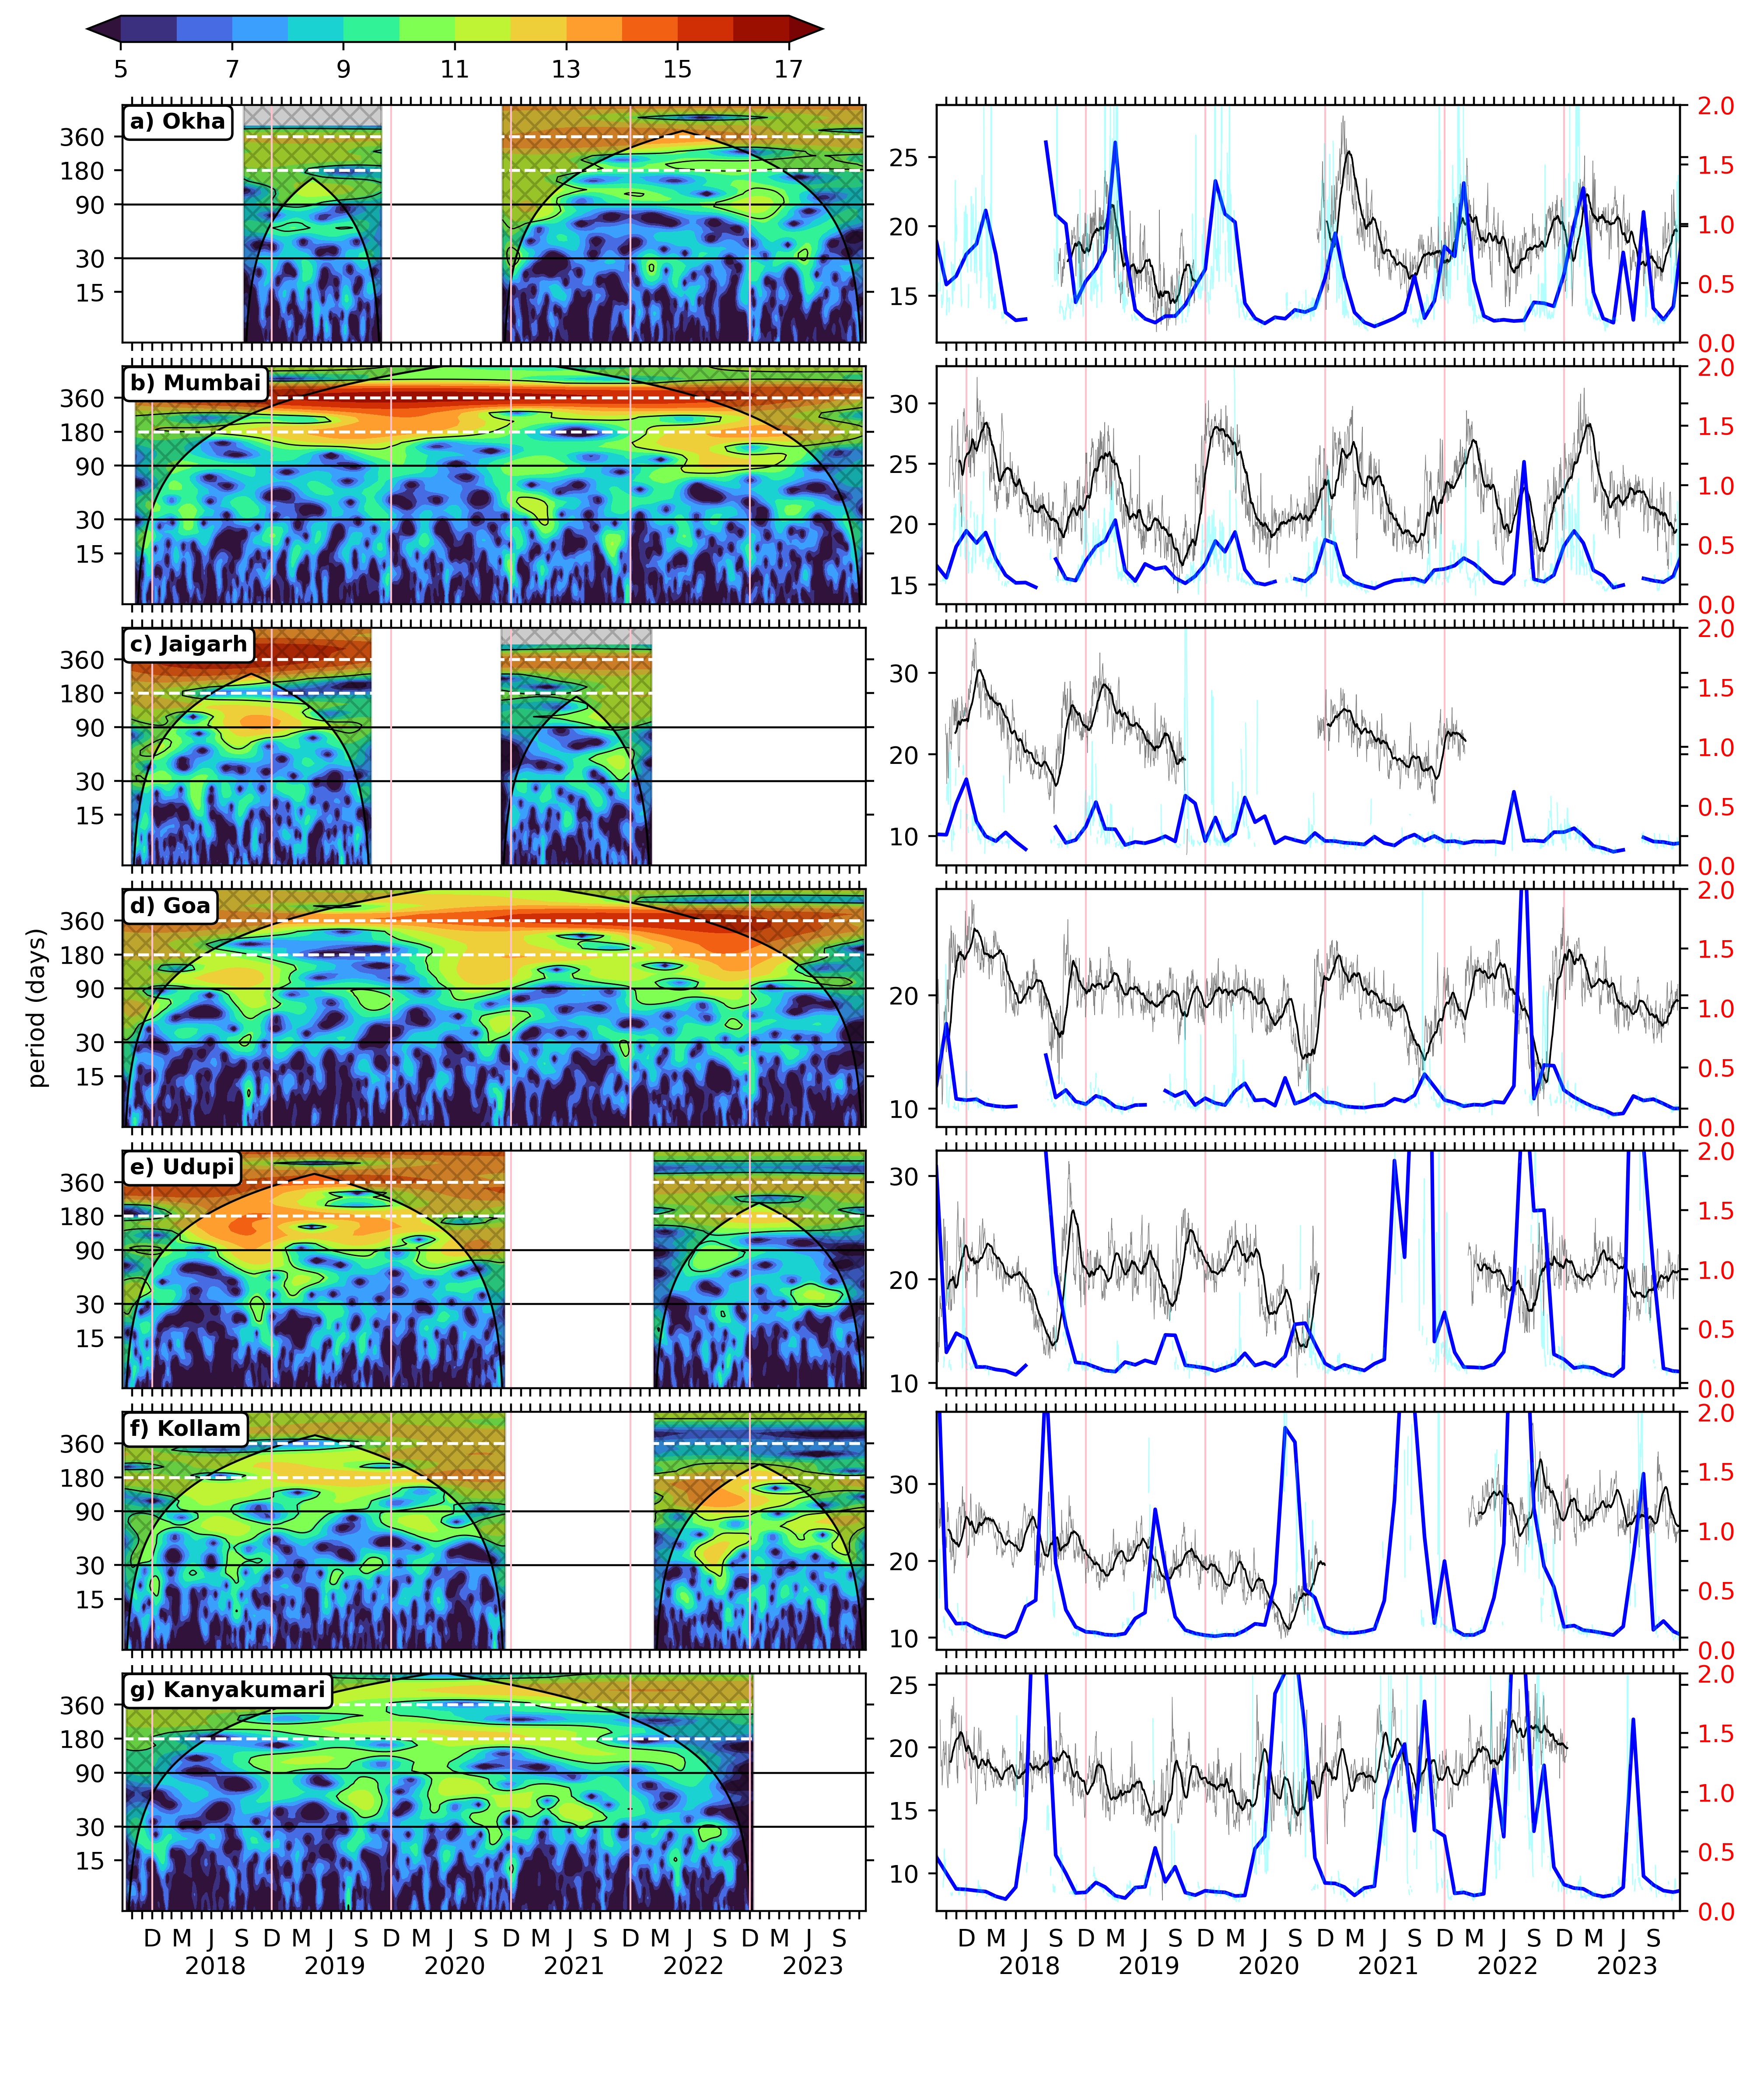
\includegraphics[width=\textwidth]{/media/scilab/disk_ranjan/works/backscatter_wc/figures/west_coast_wavelet_ss_chl.png} 
	\captionsetup{justification=justified,font=footnotesize,skip=0.05\baselineskip,width=\textwidth}
	\caption{Wavelet power spectra (Morlet) of zooplankton standing stock plotted against time as abscissa and period in days as ordinate. The wavelet power is in log$_2$ scale, the 95 \% significance is marked in black contours; The vertical white lines separates years. The right side panel shows the ZSS time series of 30 day rolling mean data (black)overlaid upon daily data (Grey). The 30 day rolling mean data of chlorophyll (solid blue line) is plotted over its daily data (cyan).}
	\label{fig:wavess}
\end{figure}



%\begin{figure}[htbp]
%	\centering
%	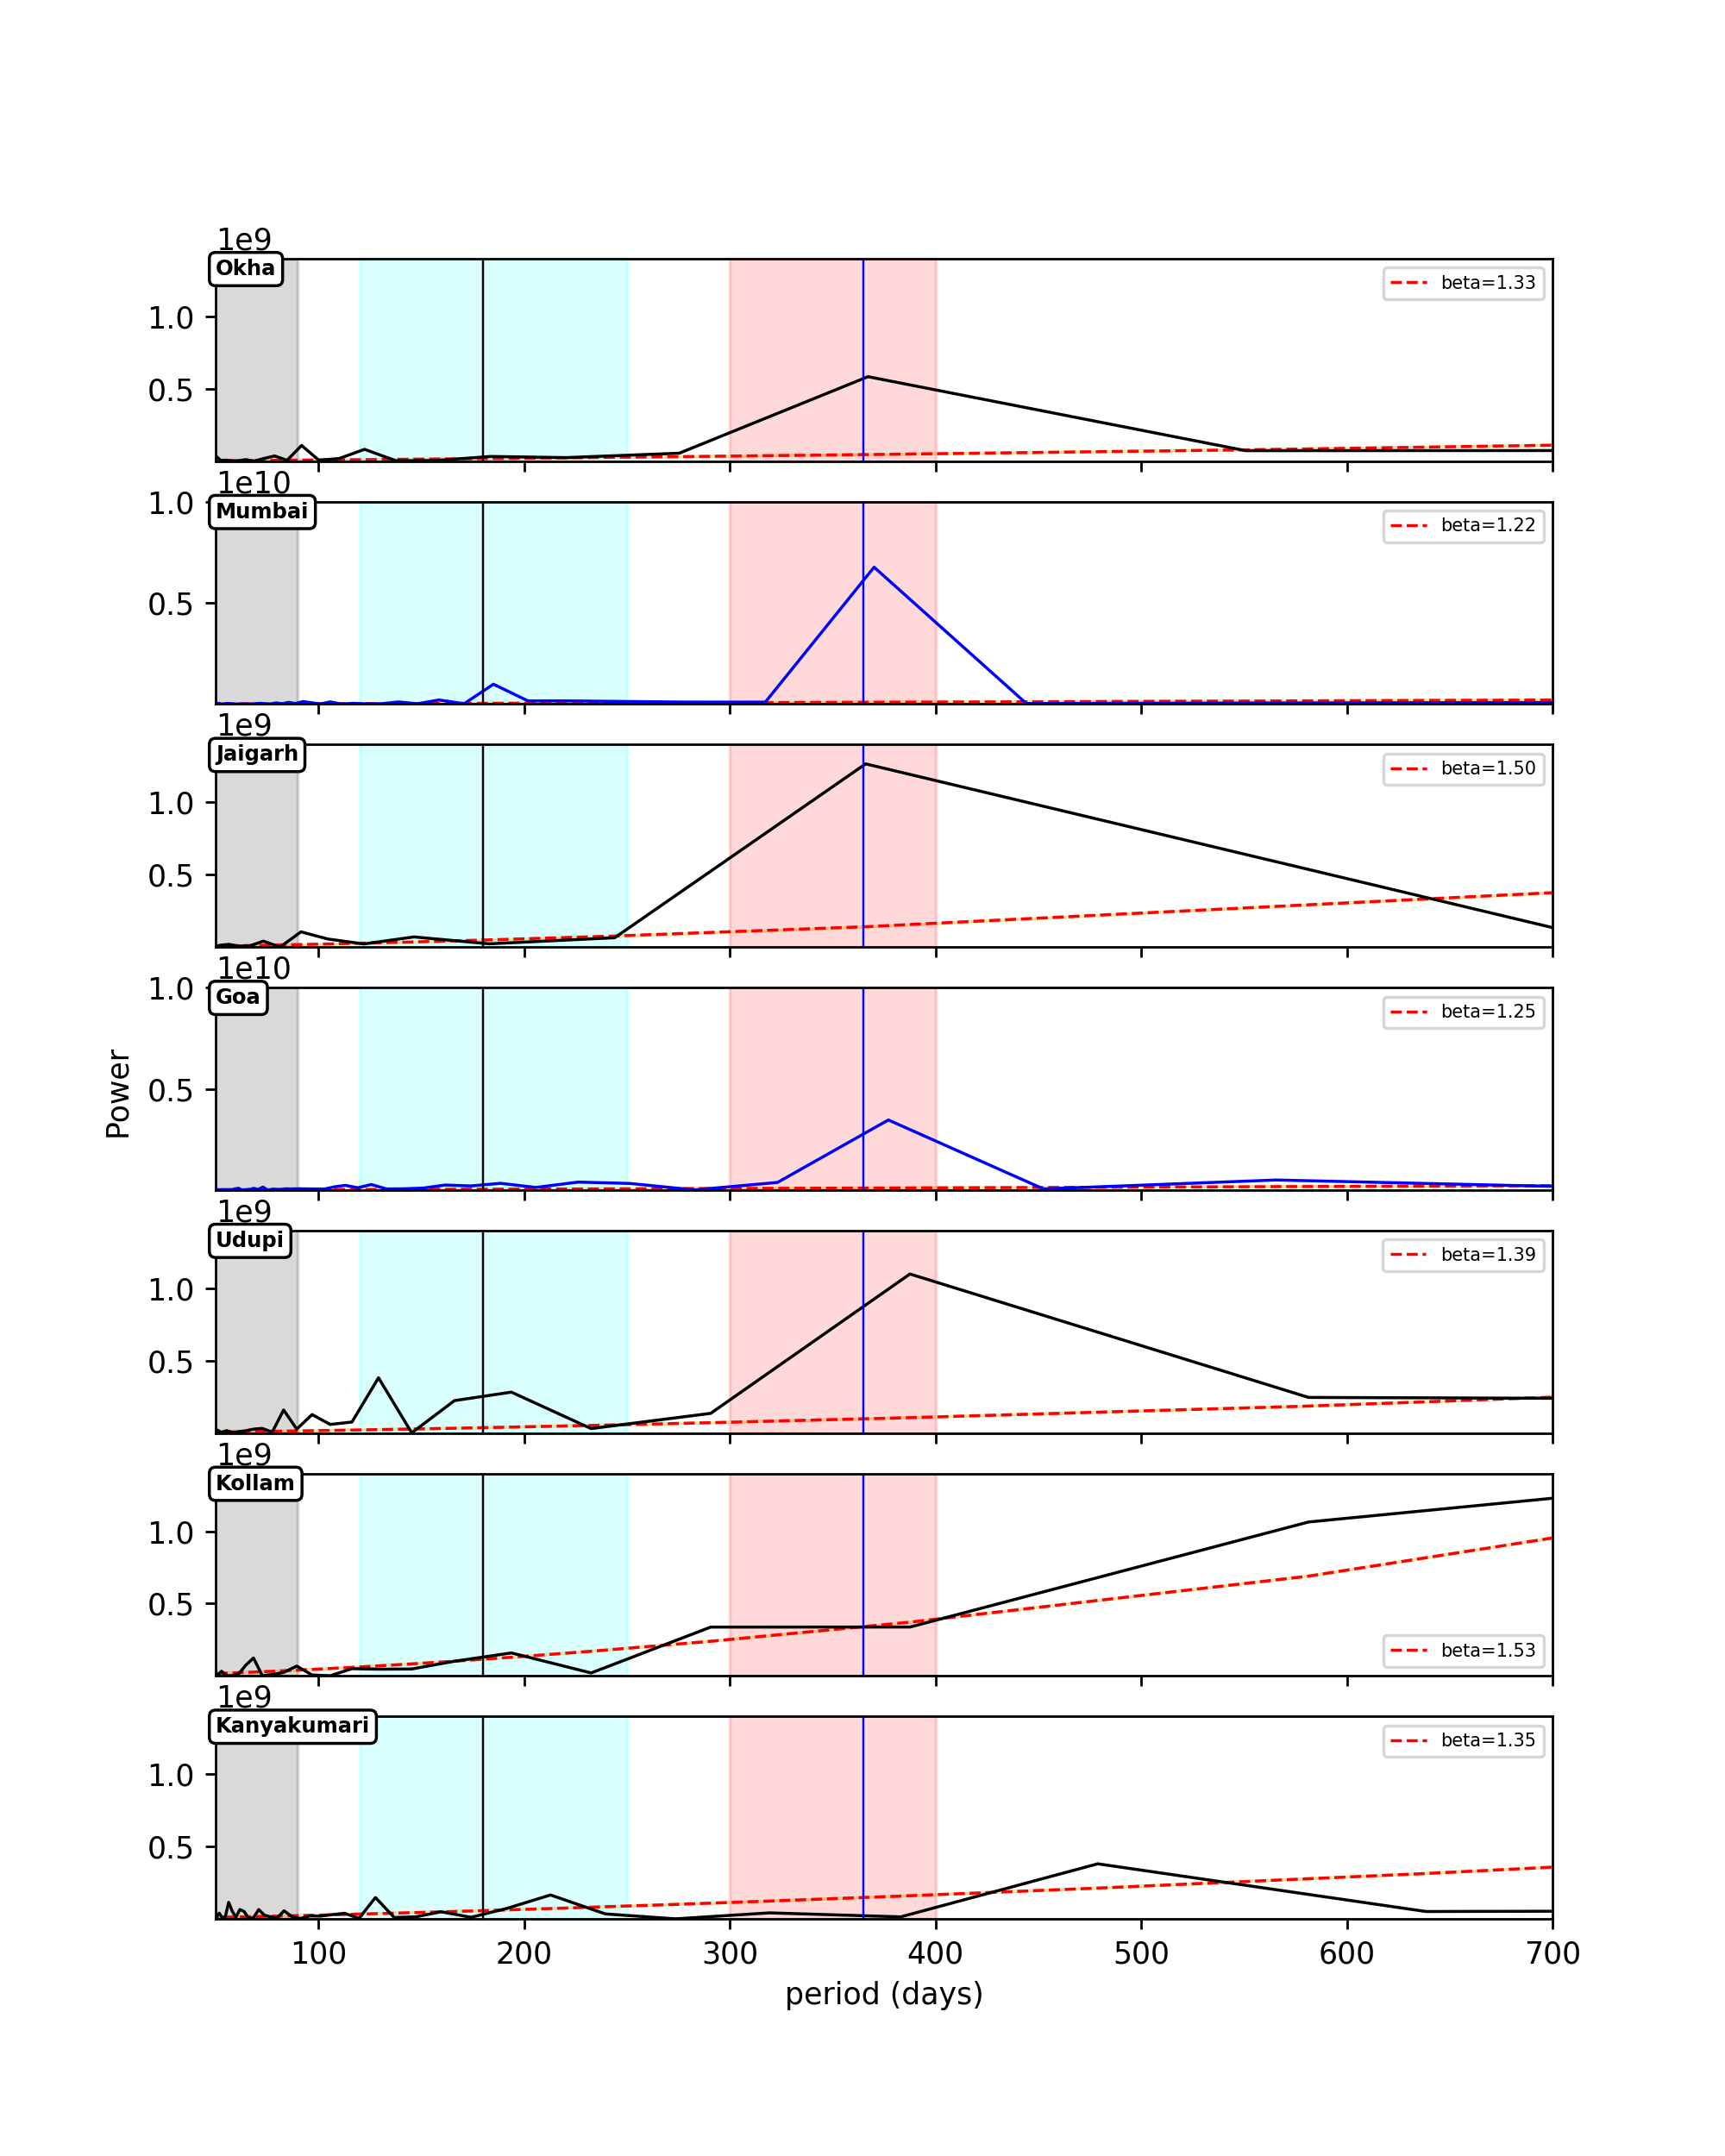
\includegraphics[width=\textwidth]{/media/scilab/disk_ranjan/works/backscatter_wc/figures/west_coast_fft_ss.png} 
%	\captionsetup{justification=justified,font=footnotesize,skip=0.05\baselineskip,width=\textwidth}
%	\caption{FFT of the ZSS time series data. On the event of discontinuity in data record, the longest available of respective location is considered for analysis. The black (blue) curve is fft power with scale $10^{9}$  ($10^{10}$). The Grey, cyan and pink spans the intra-seasonal, seasonal and annual bands, respectively. The red dashed curved is the red noise spectra which depends on the number of records of each location, and beta determines power contribution of the higher and lower frequencies. The vertical blue line marks the annual cycle.}
%	\label{fig:zssfft}
%\end{figure}

\begin{figure}[htbp]
	\centering
	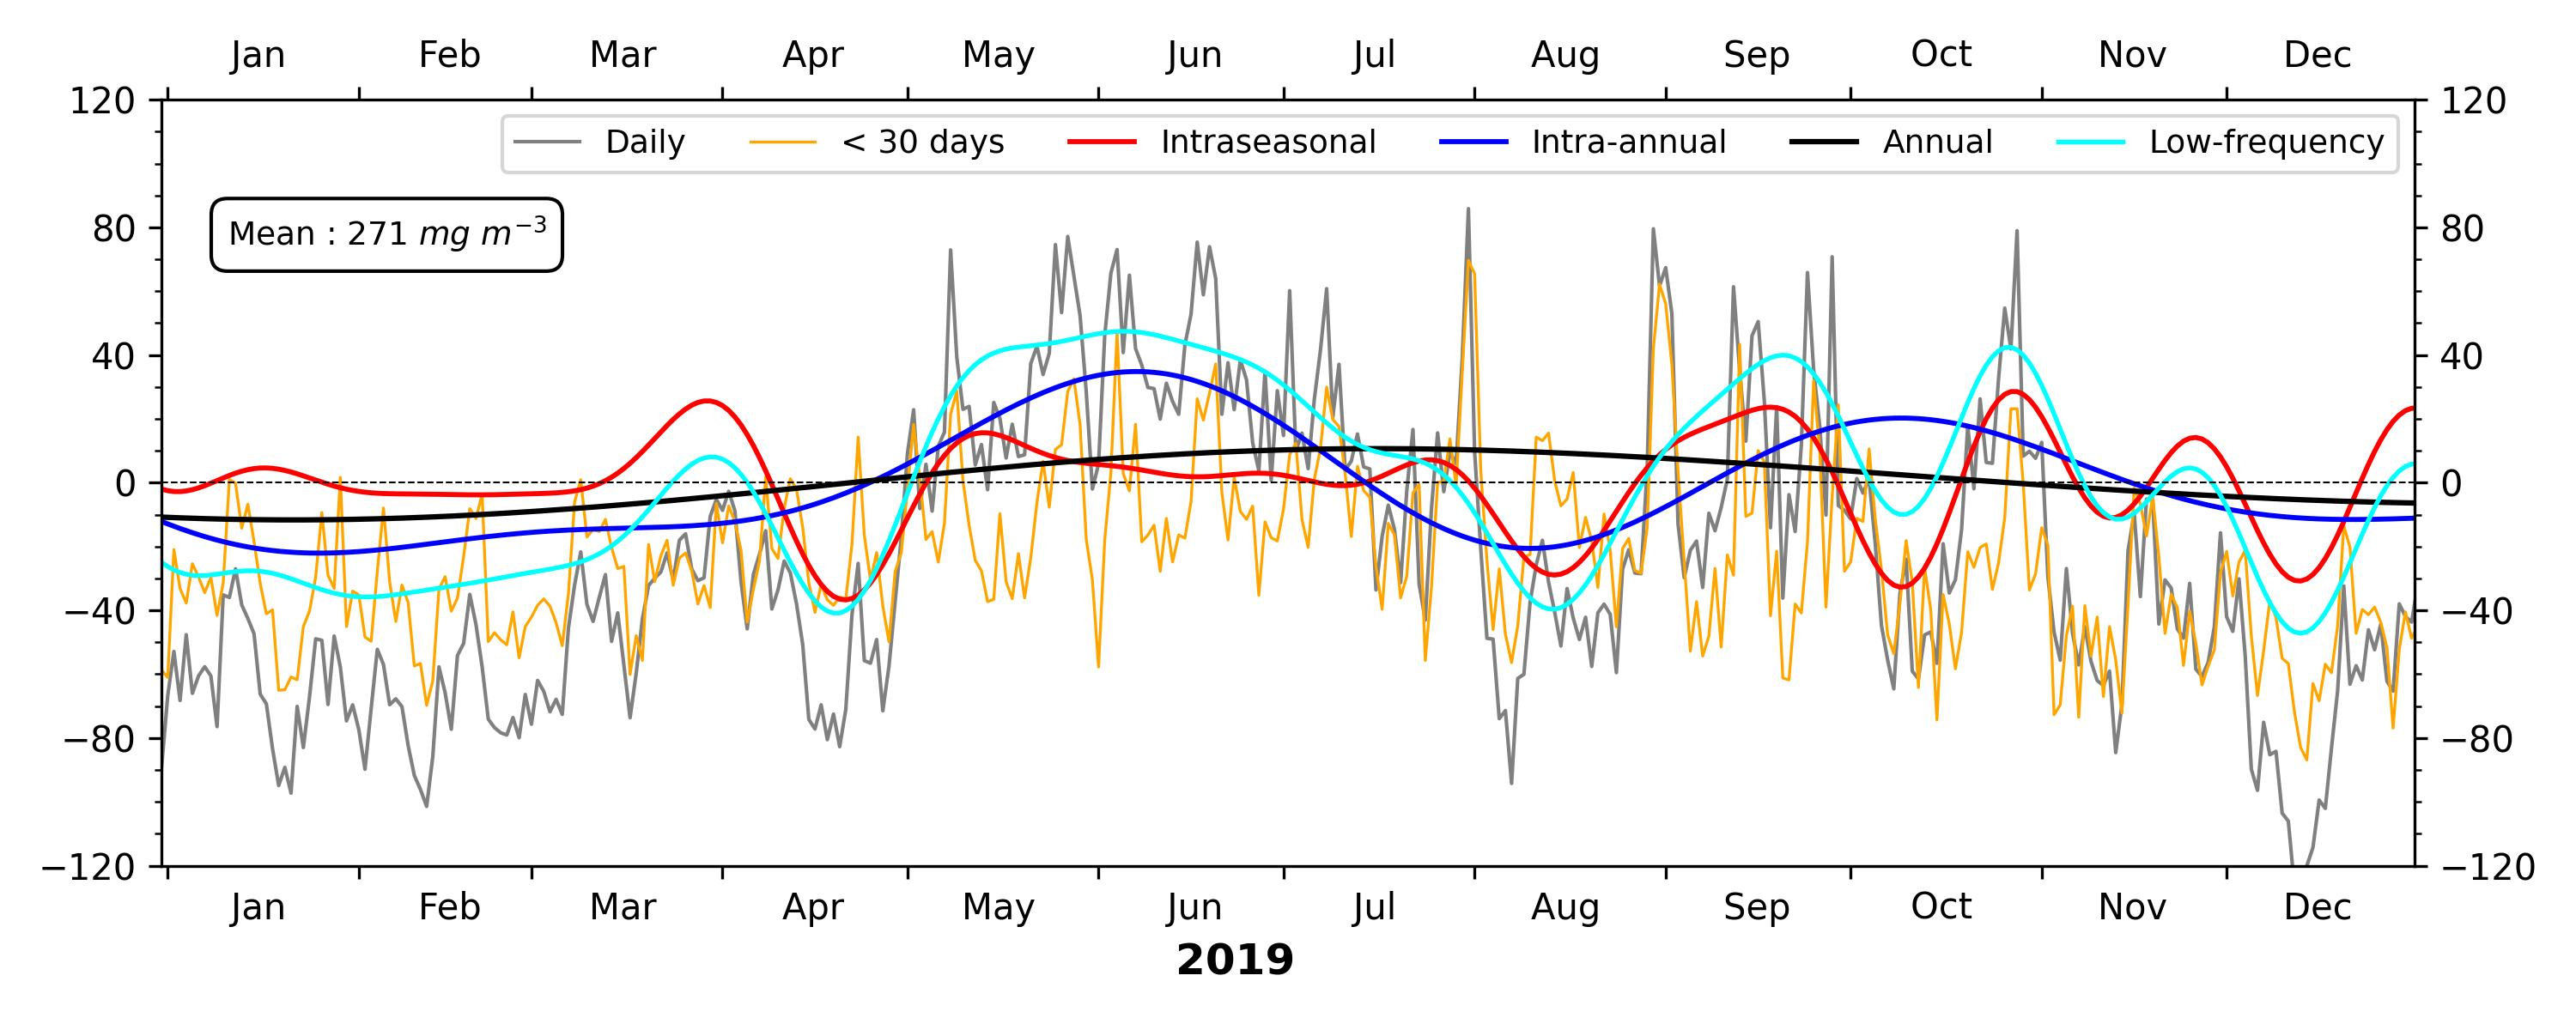
\includegraphics[width=\textwidth]{/media/scilab/disk_ranjan/works/backscatter_wc/figures/biomass_40m_2019_Kollam_l1.jpeg} 
	\captionsetup{justification=justified,font=footnotesize,skip=0.05\baselineskip,width=\textwidth}
	\caption{Comparison between mean-removed daily biomass time series at 40 m and the distinct components of variability off Kollam for 2019. The biomass units are $mg \ m^{-3}$. An increase in biomass is noticed from May onward and lasting till late monsoon with weeks of low biomass during August due to contribution from each component of variability. The cyan curve is sum of all low frequency components above 30 days, i.e, annual, intra-annual and 30 to 90 days intraseasonal variability.}
	\label{fig:variability}
\end{figure}

\begin{figure}[htbp]
	\centering
	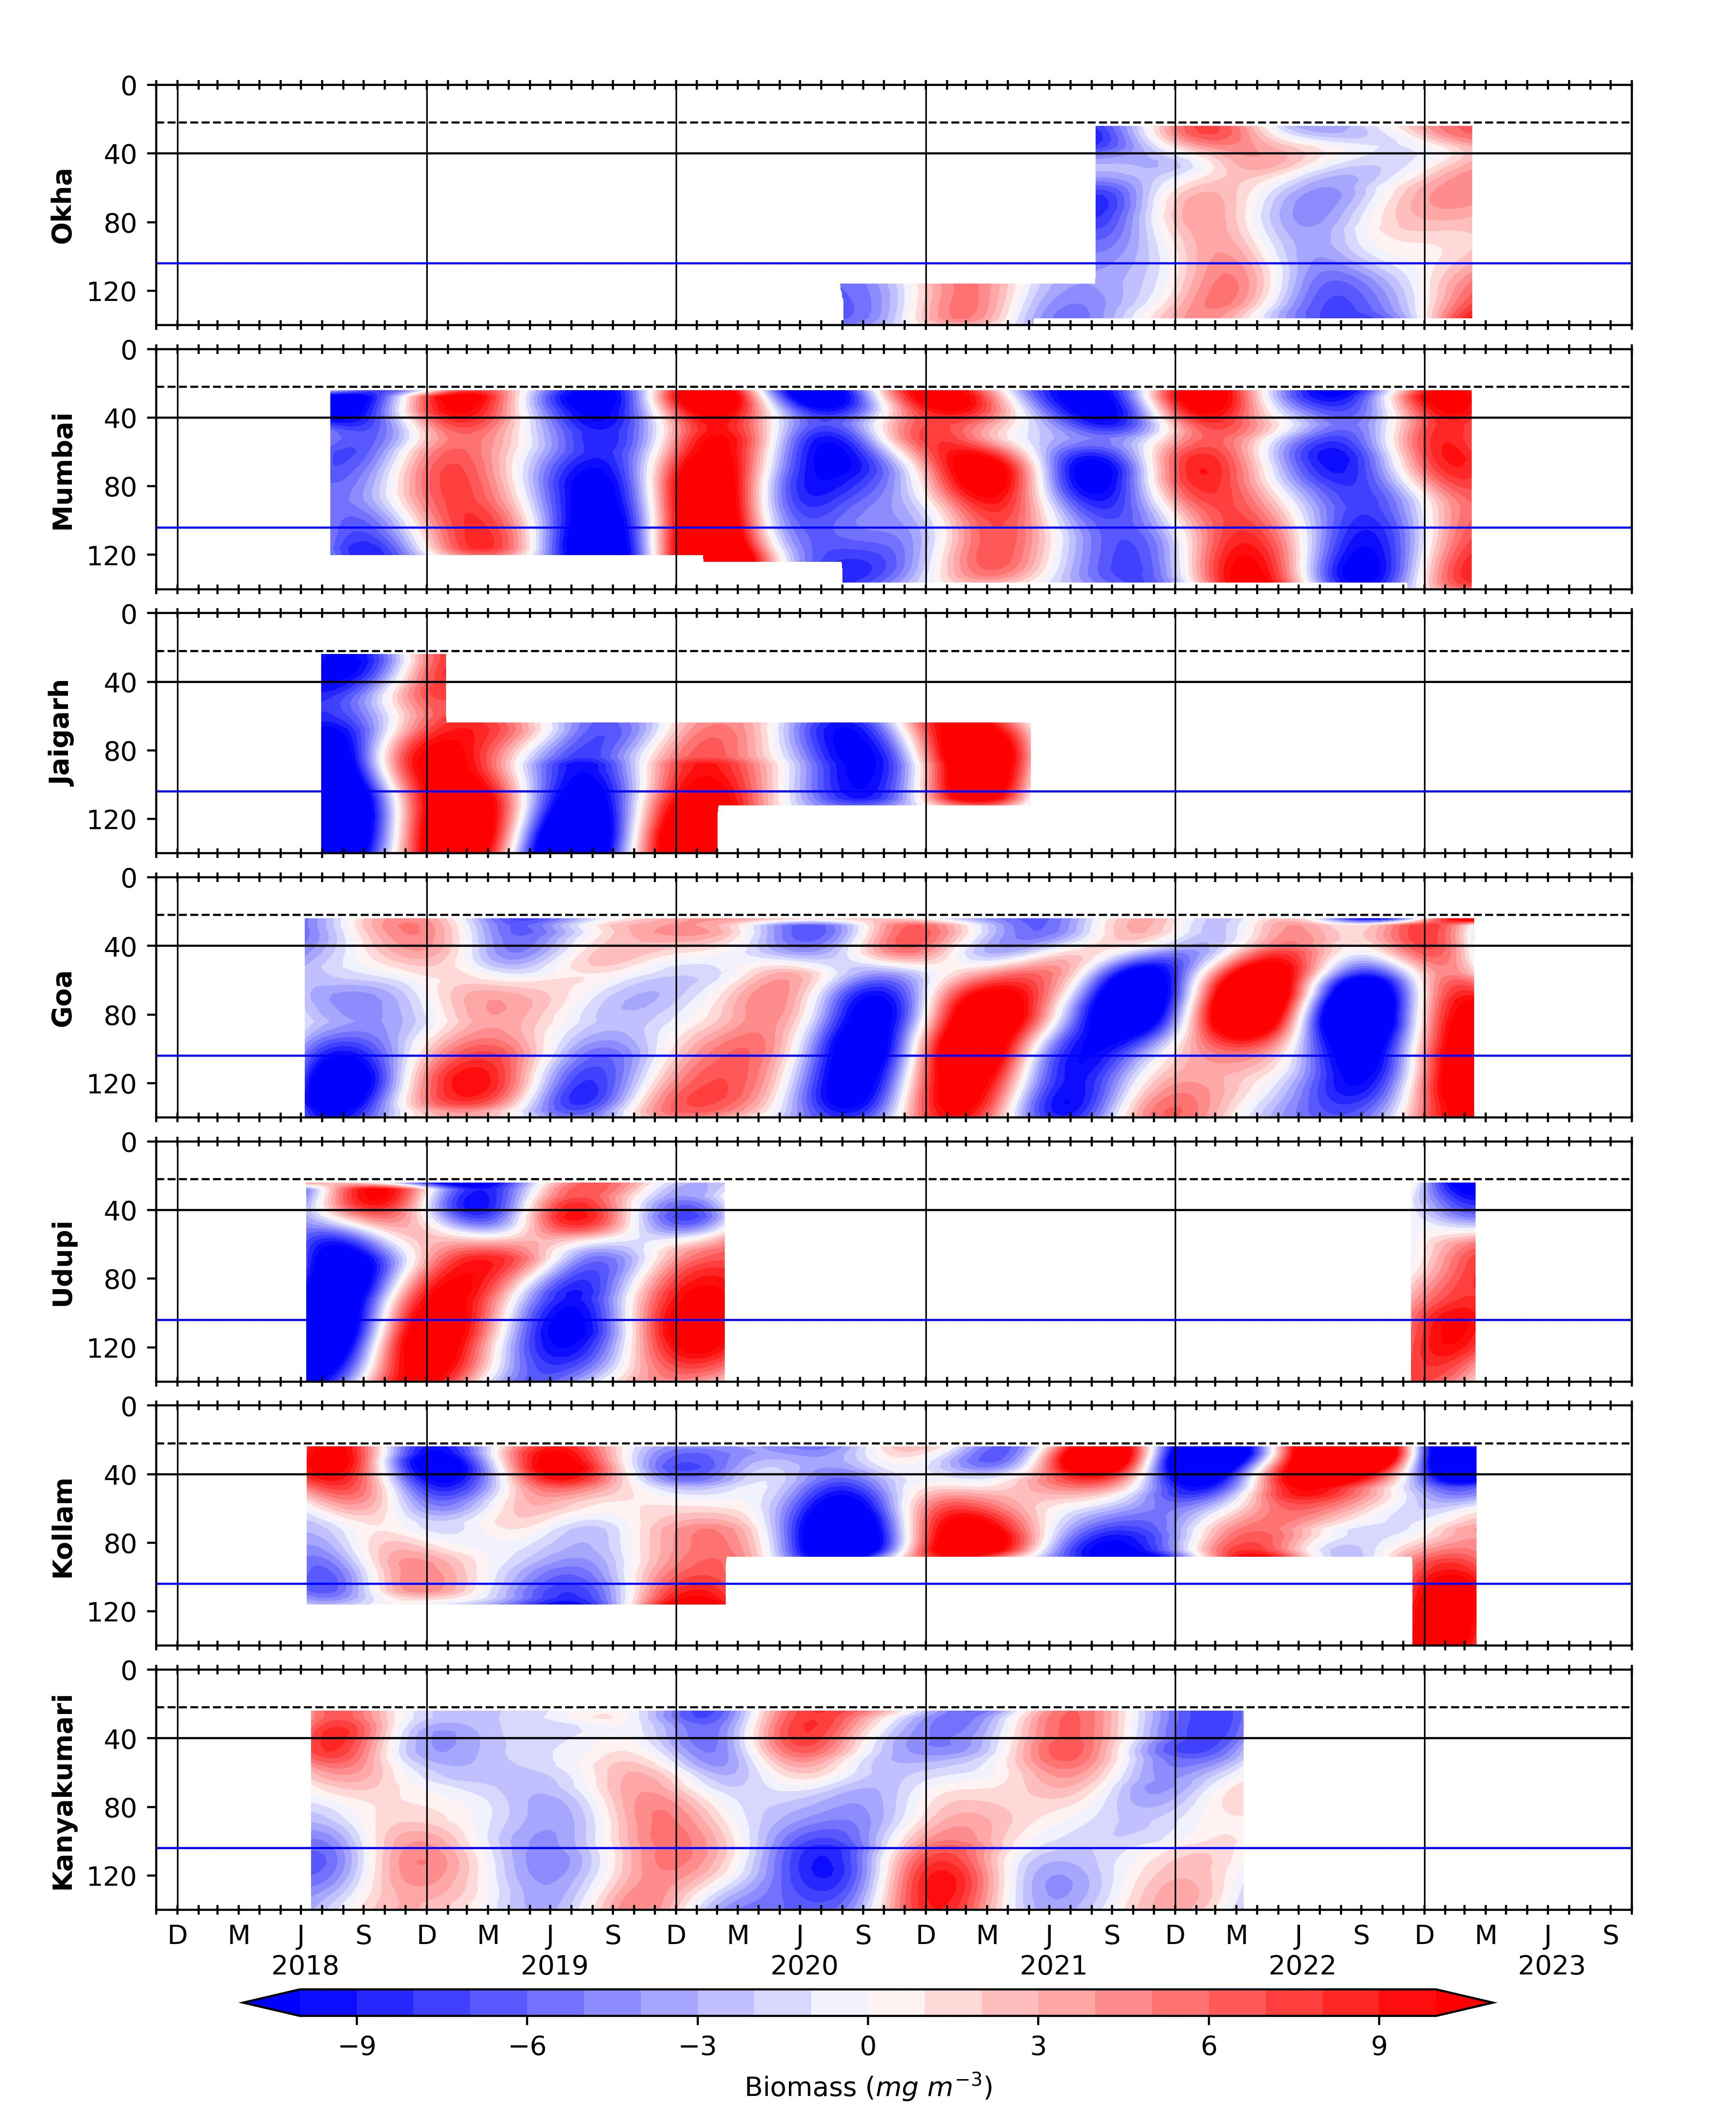
\includegraphics[width=1.05\textwidth]{/media/scilab/disk_ranjan/works/backscatter_wc/figures/annual_300_400_451_1.jpeg} 
	\captionsetup{justification=justified,font=footnotesize,skip=0.05\baselineskip,width=\textwidth}
	\caption{The biomass variation occurring in annual band (300 to 400 days). Owing to the presence of monsoon, there is a variation driven by associated upwelling (downwelling) processes in summer (winter) monsoon. and The horizontal black and blue lines is for 40 and 104 m respectively; vertical black lines separate the years. The dashed line at 22 m marks the top-depth of first bin i.e, 24 m and solid orange curves denotes D215 (D175 off Okha and Kanyakumari)}
	\label{fig:annual}
\end{figure}

\begin{figure}[htbp]
	\centering
	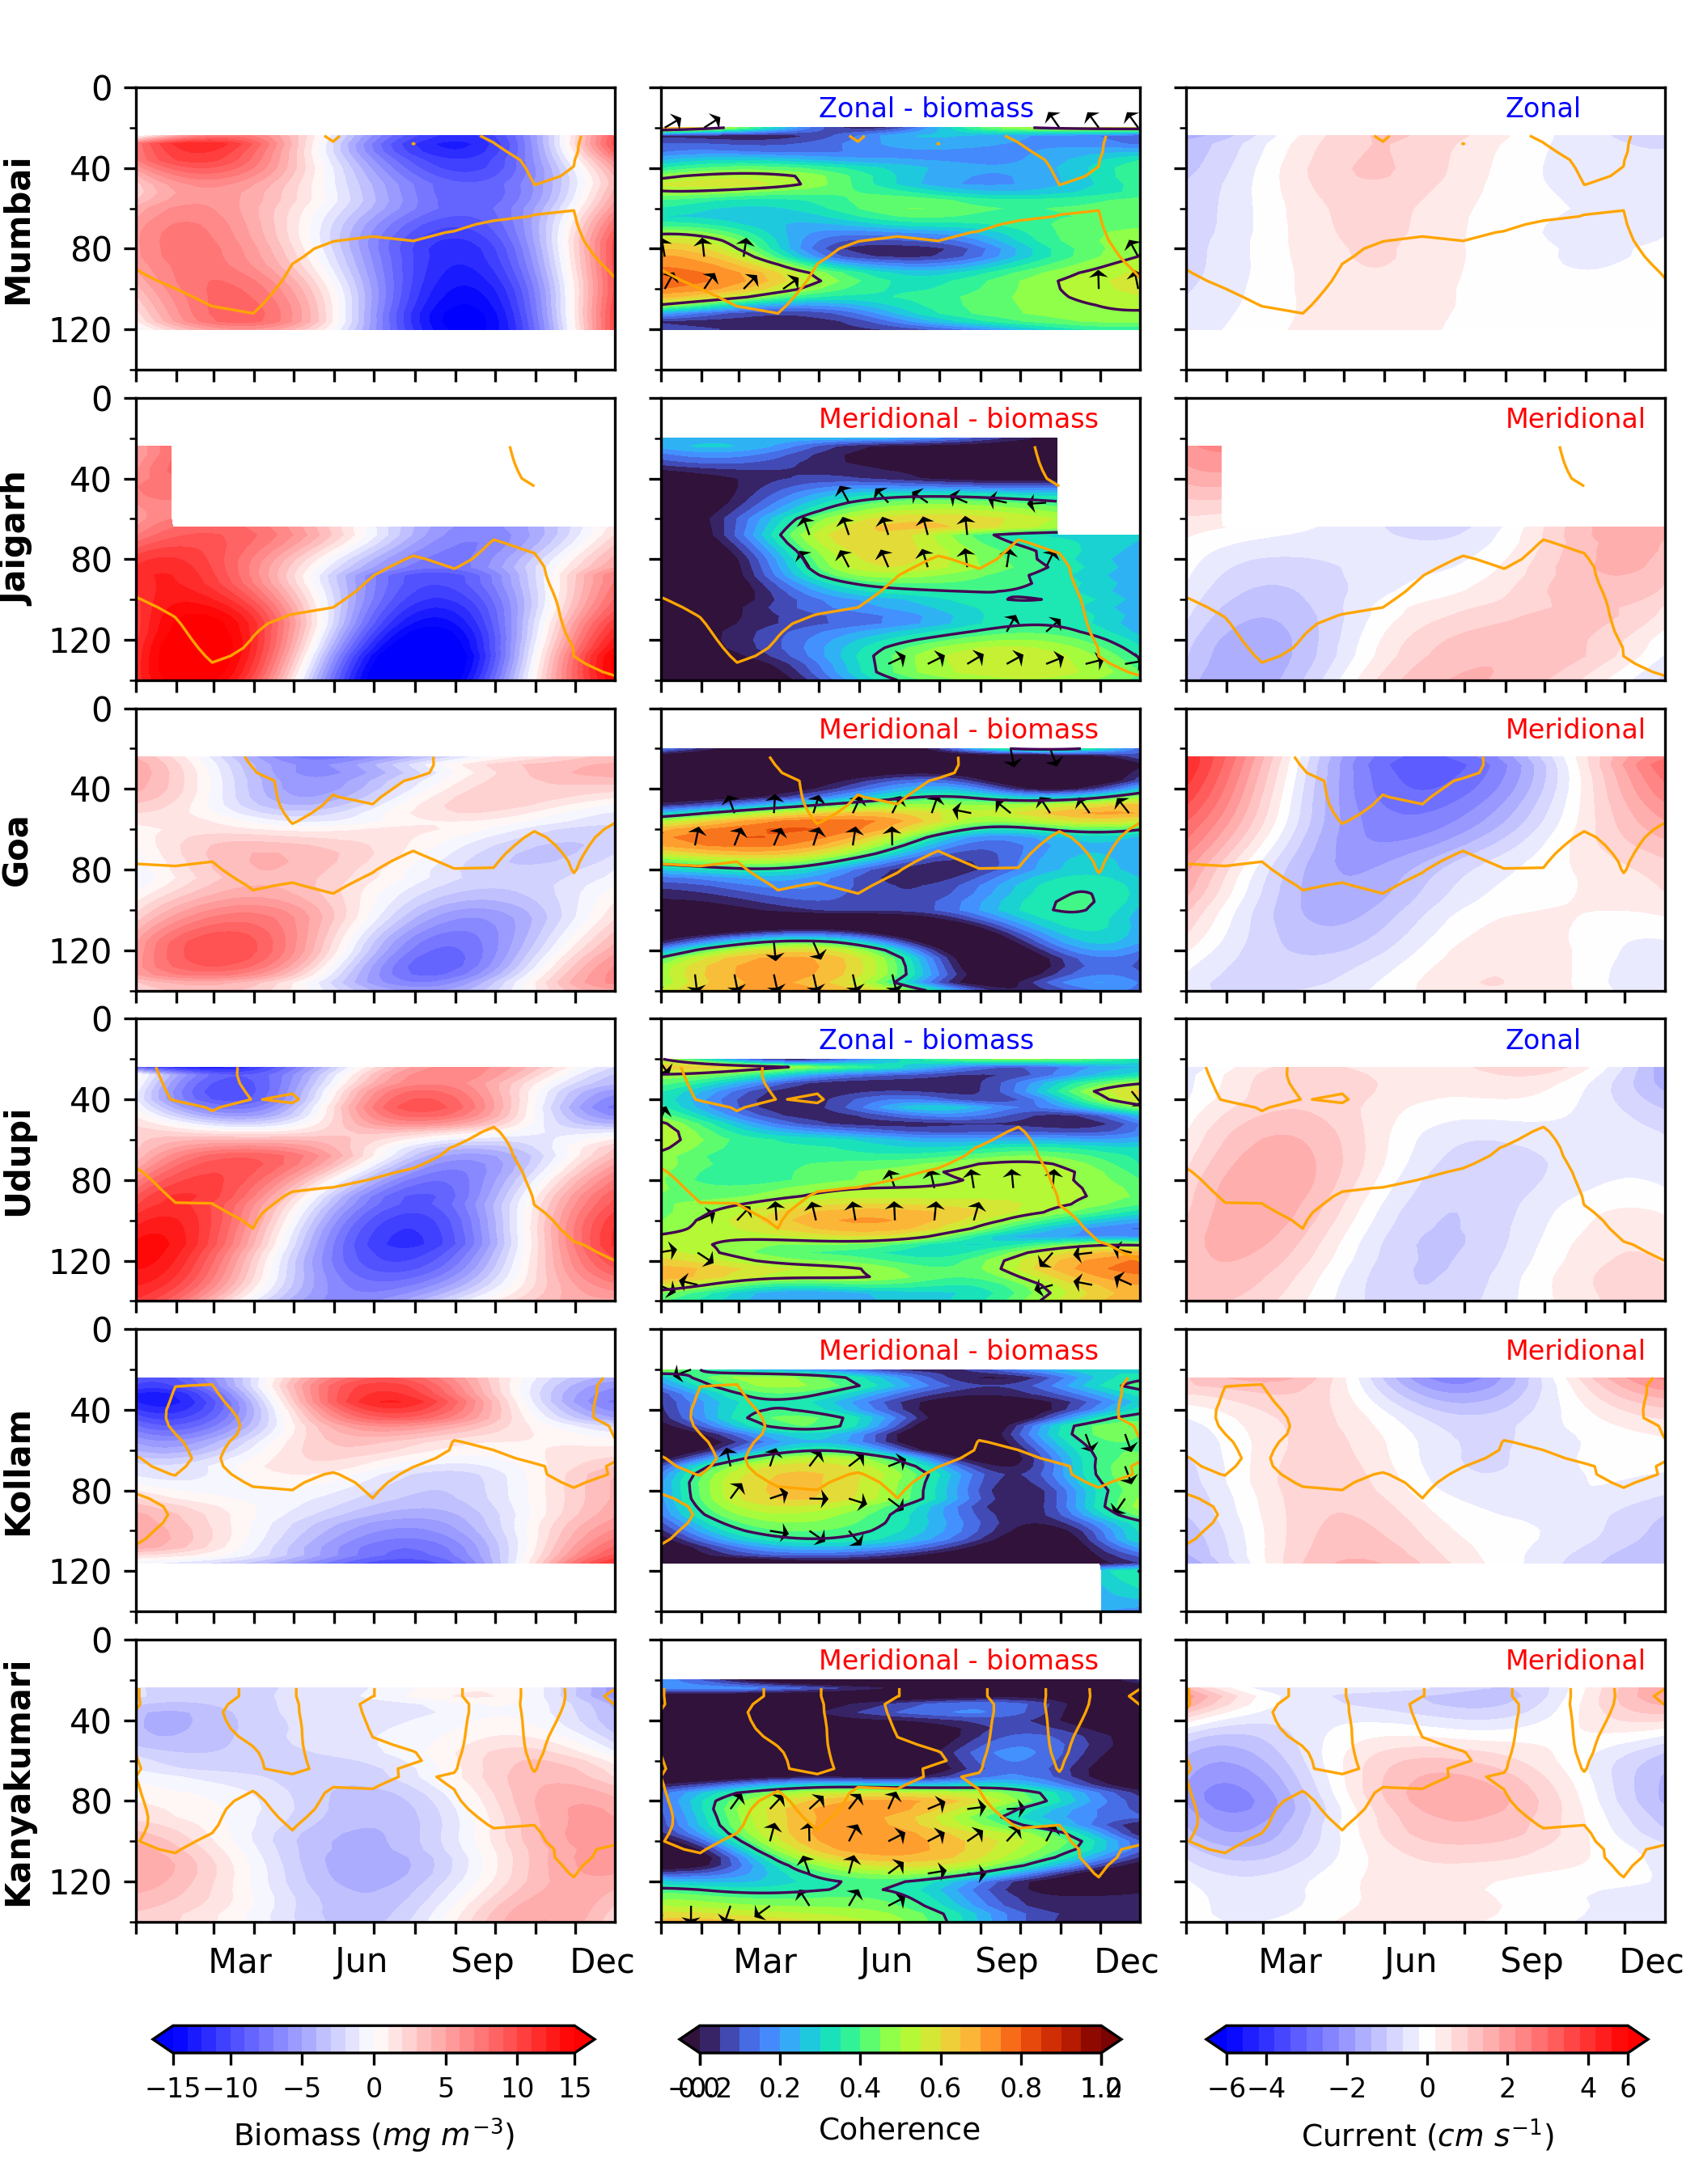
\includegraphics[width=0.9\textwidth]{/media/scilab/disk_ranjan/works/backscatter_wc/figures/Current_biomass_and_coherence_2019.png} 
	\captionsetup{justification=justified,font=footnotesize,skip=0.05\baselineskip,width=\textwidth}
	\caption{Current (zonal/meridional) and biomass wavelet coherence plotted alongside of annual filtered biomass and current. Either zonal or meridional current is considered depending on coherence and if current leads biomass. The solid contour encompasses greater than 0.5 coherence and phase is plotted with north as reference, +ve (-ve) x-axis is current leading (lagging) biomass. Left (Right) panel is for biomass (current). Although the annual biomass variability is weak and contributes less to the total biomass time series, upward phase propagation is seen implying upwelling favorable conditions leading to biomass growth. The solid orange curves denotes D215 (D175 off Okha and Kanyakumari)}
	\label{fig:biomasscurrentcoh}
\end{figure}


\begin{figure}[htbp]
	\centering
	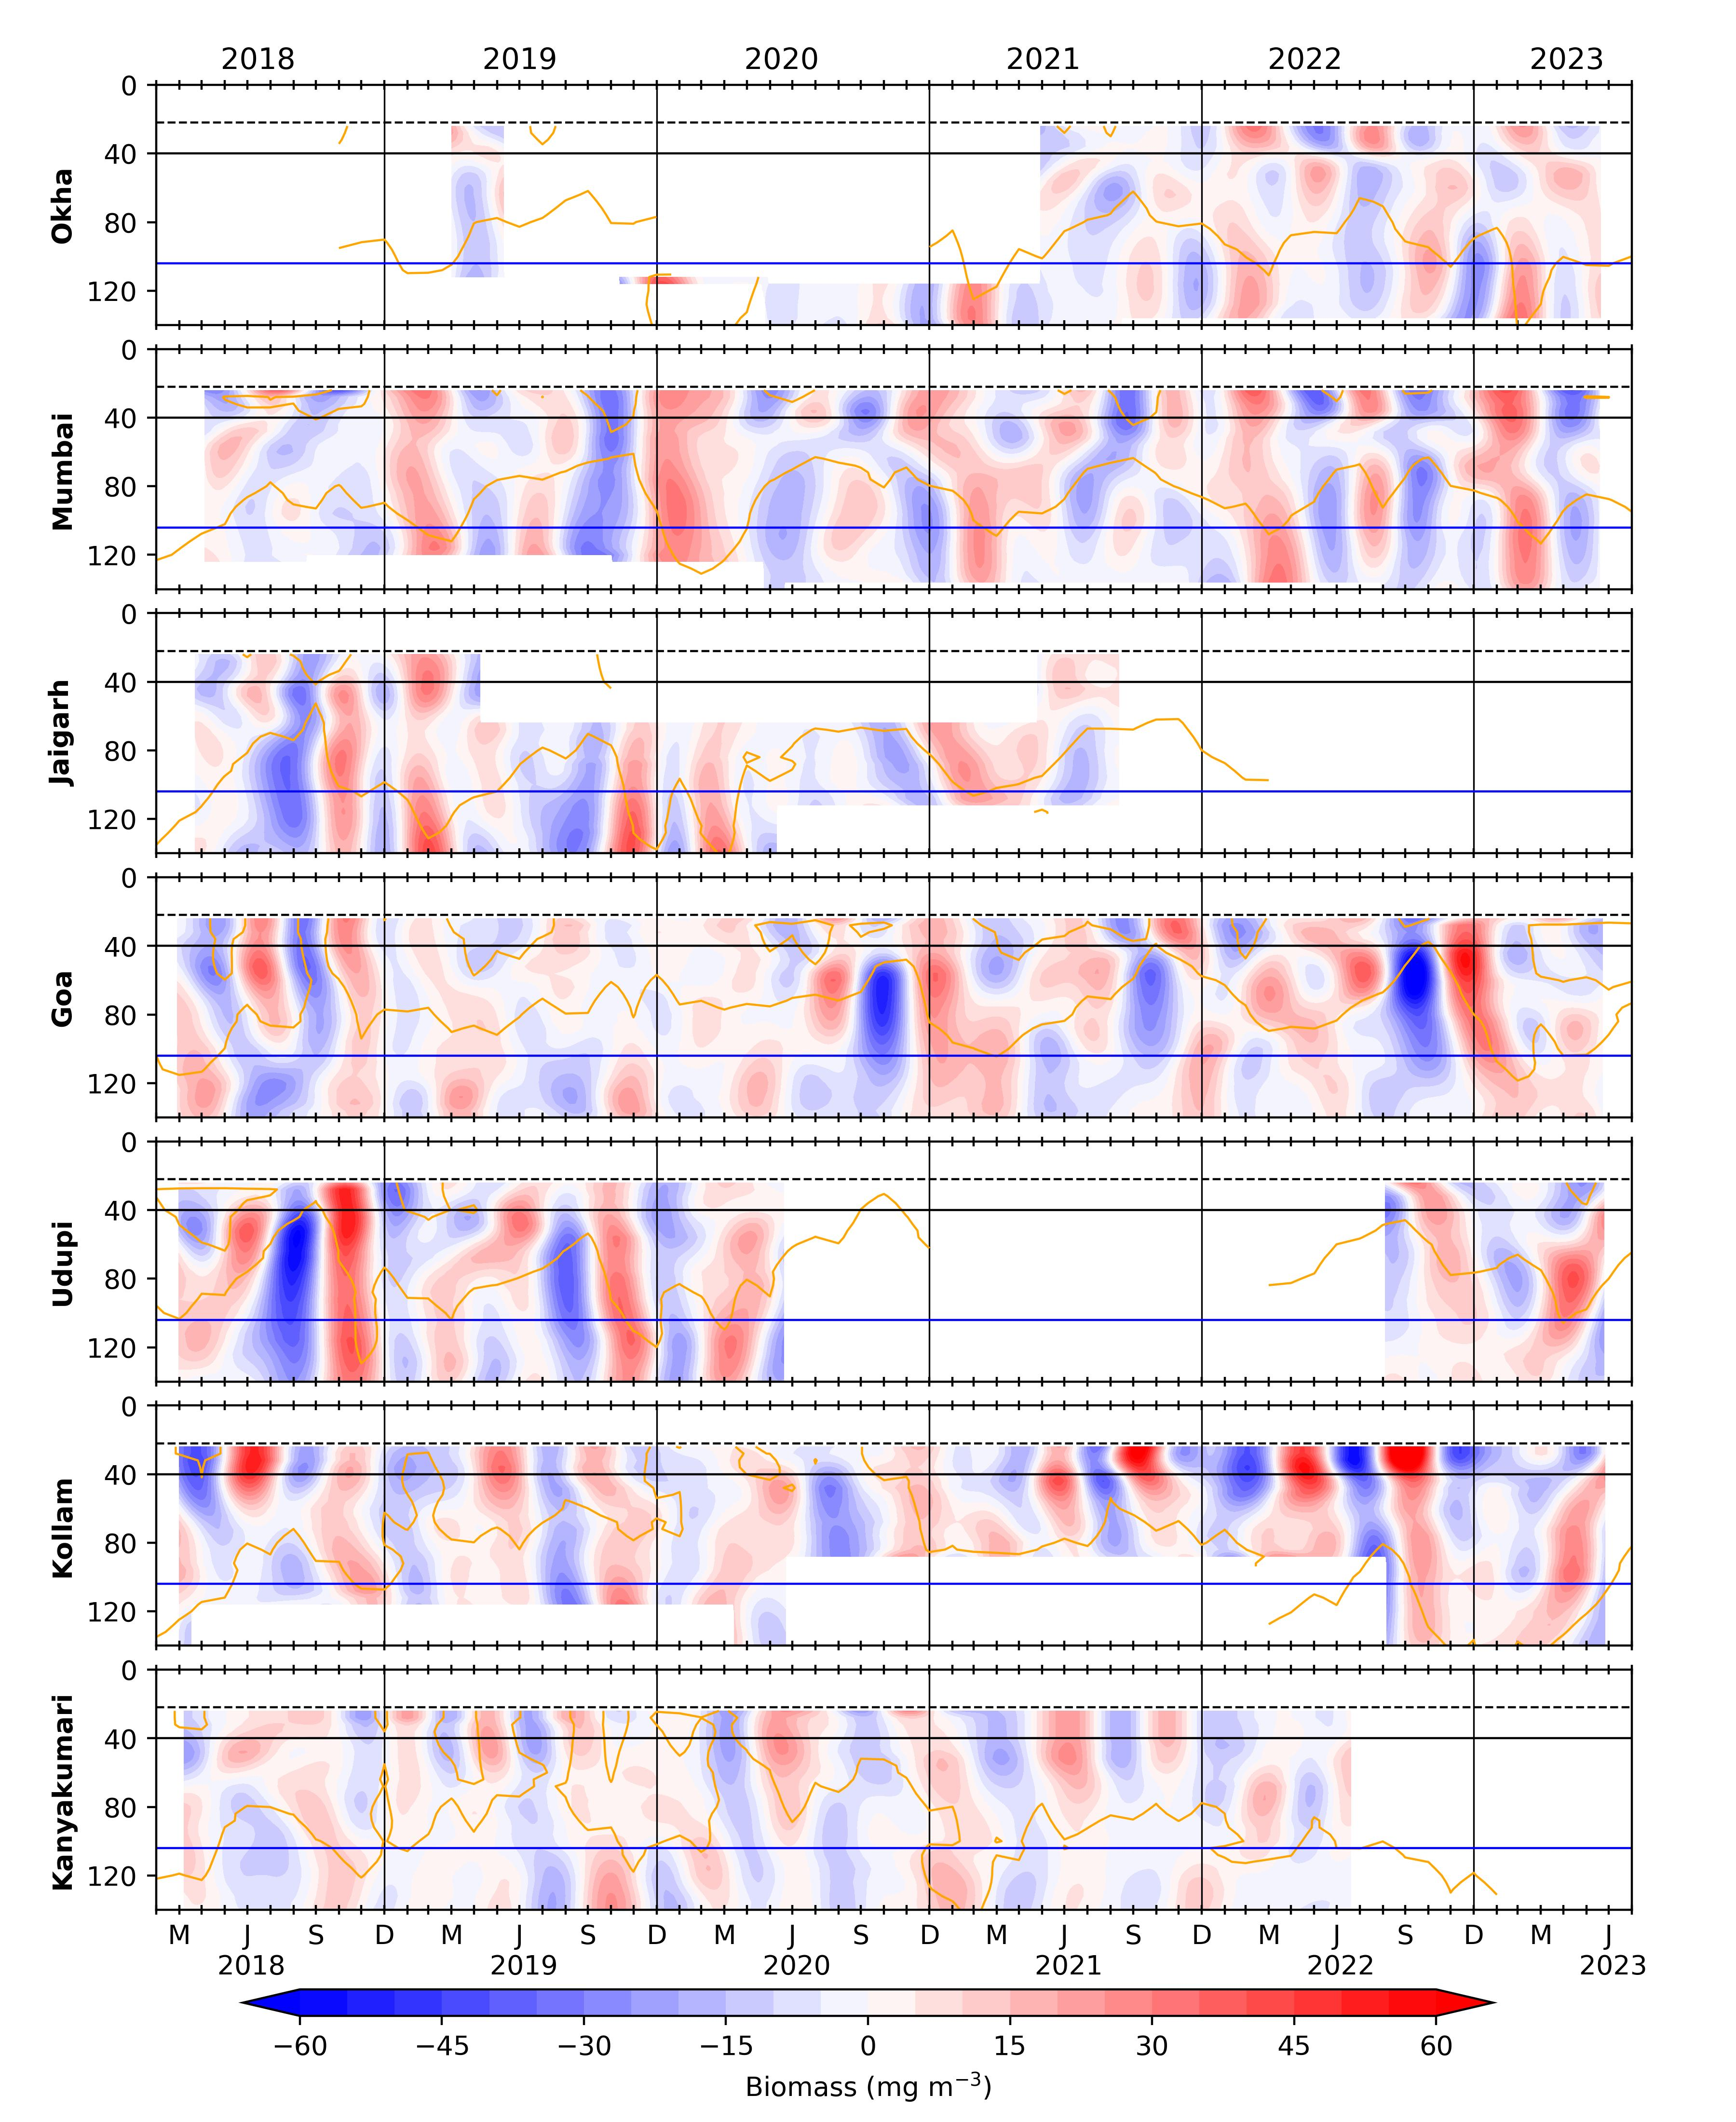
\includegraphics[width=\textwidth]{/media/scilab/disk_ranjan/works/backscatter_wc/figures/intraannual_100_250_351.jpeg} 
	\captionsetup{justification=justified,font=footnotesize,skip=0.05\baselineskip,width=\textwidth}
	\caption{The biomass variation occurring in 100 to 250 days period (between the seasons and within a year record or intra-annual band) is obtained using a band pass filter. The horizontal black and blue lines is for 40 and 104 m respectively; vertical black lines separate the years. The dashed line at 22 m marks the top-depth of first bin i.e, 24 m and solid orange curves denotes D215 (D175 off Okha and Kanyakumari). }
	\label{fig:intraannual}
\end{figure}

\begin{figure}[htbp]
	\centering
	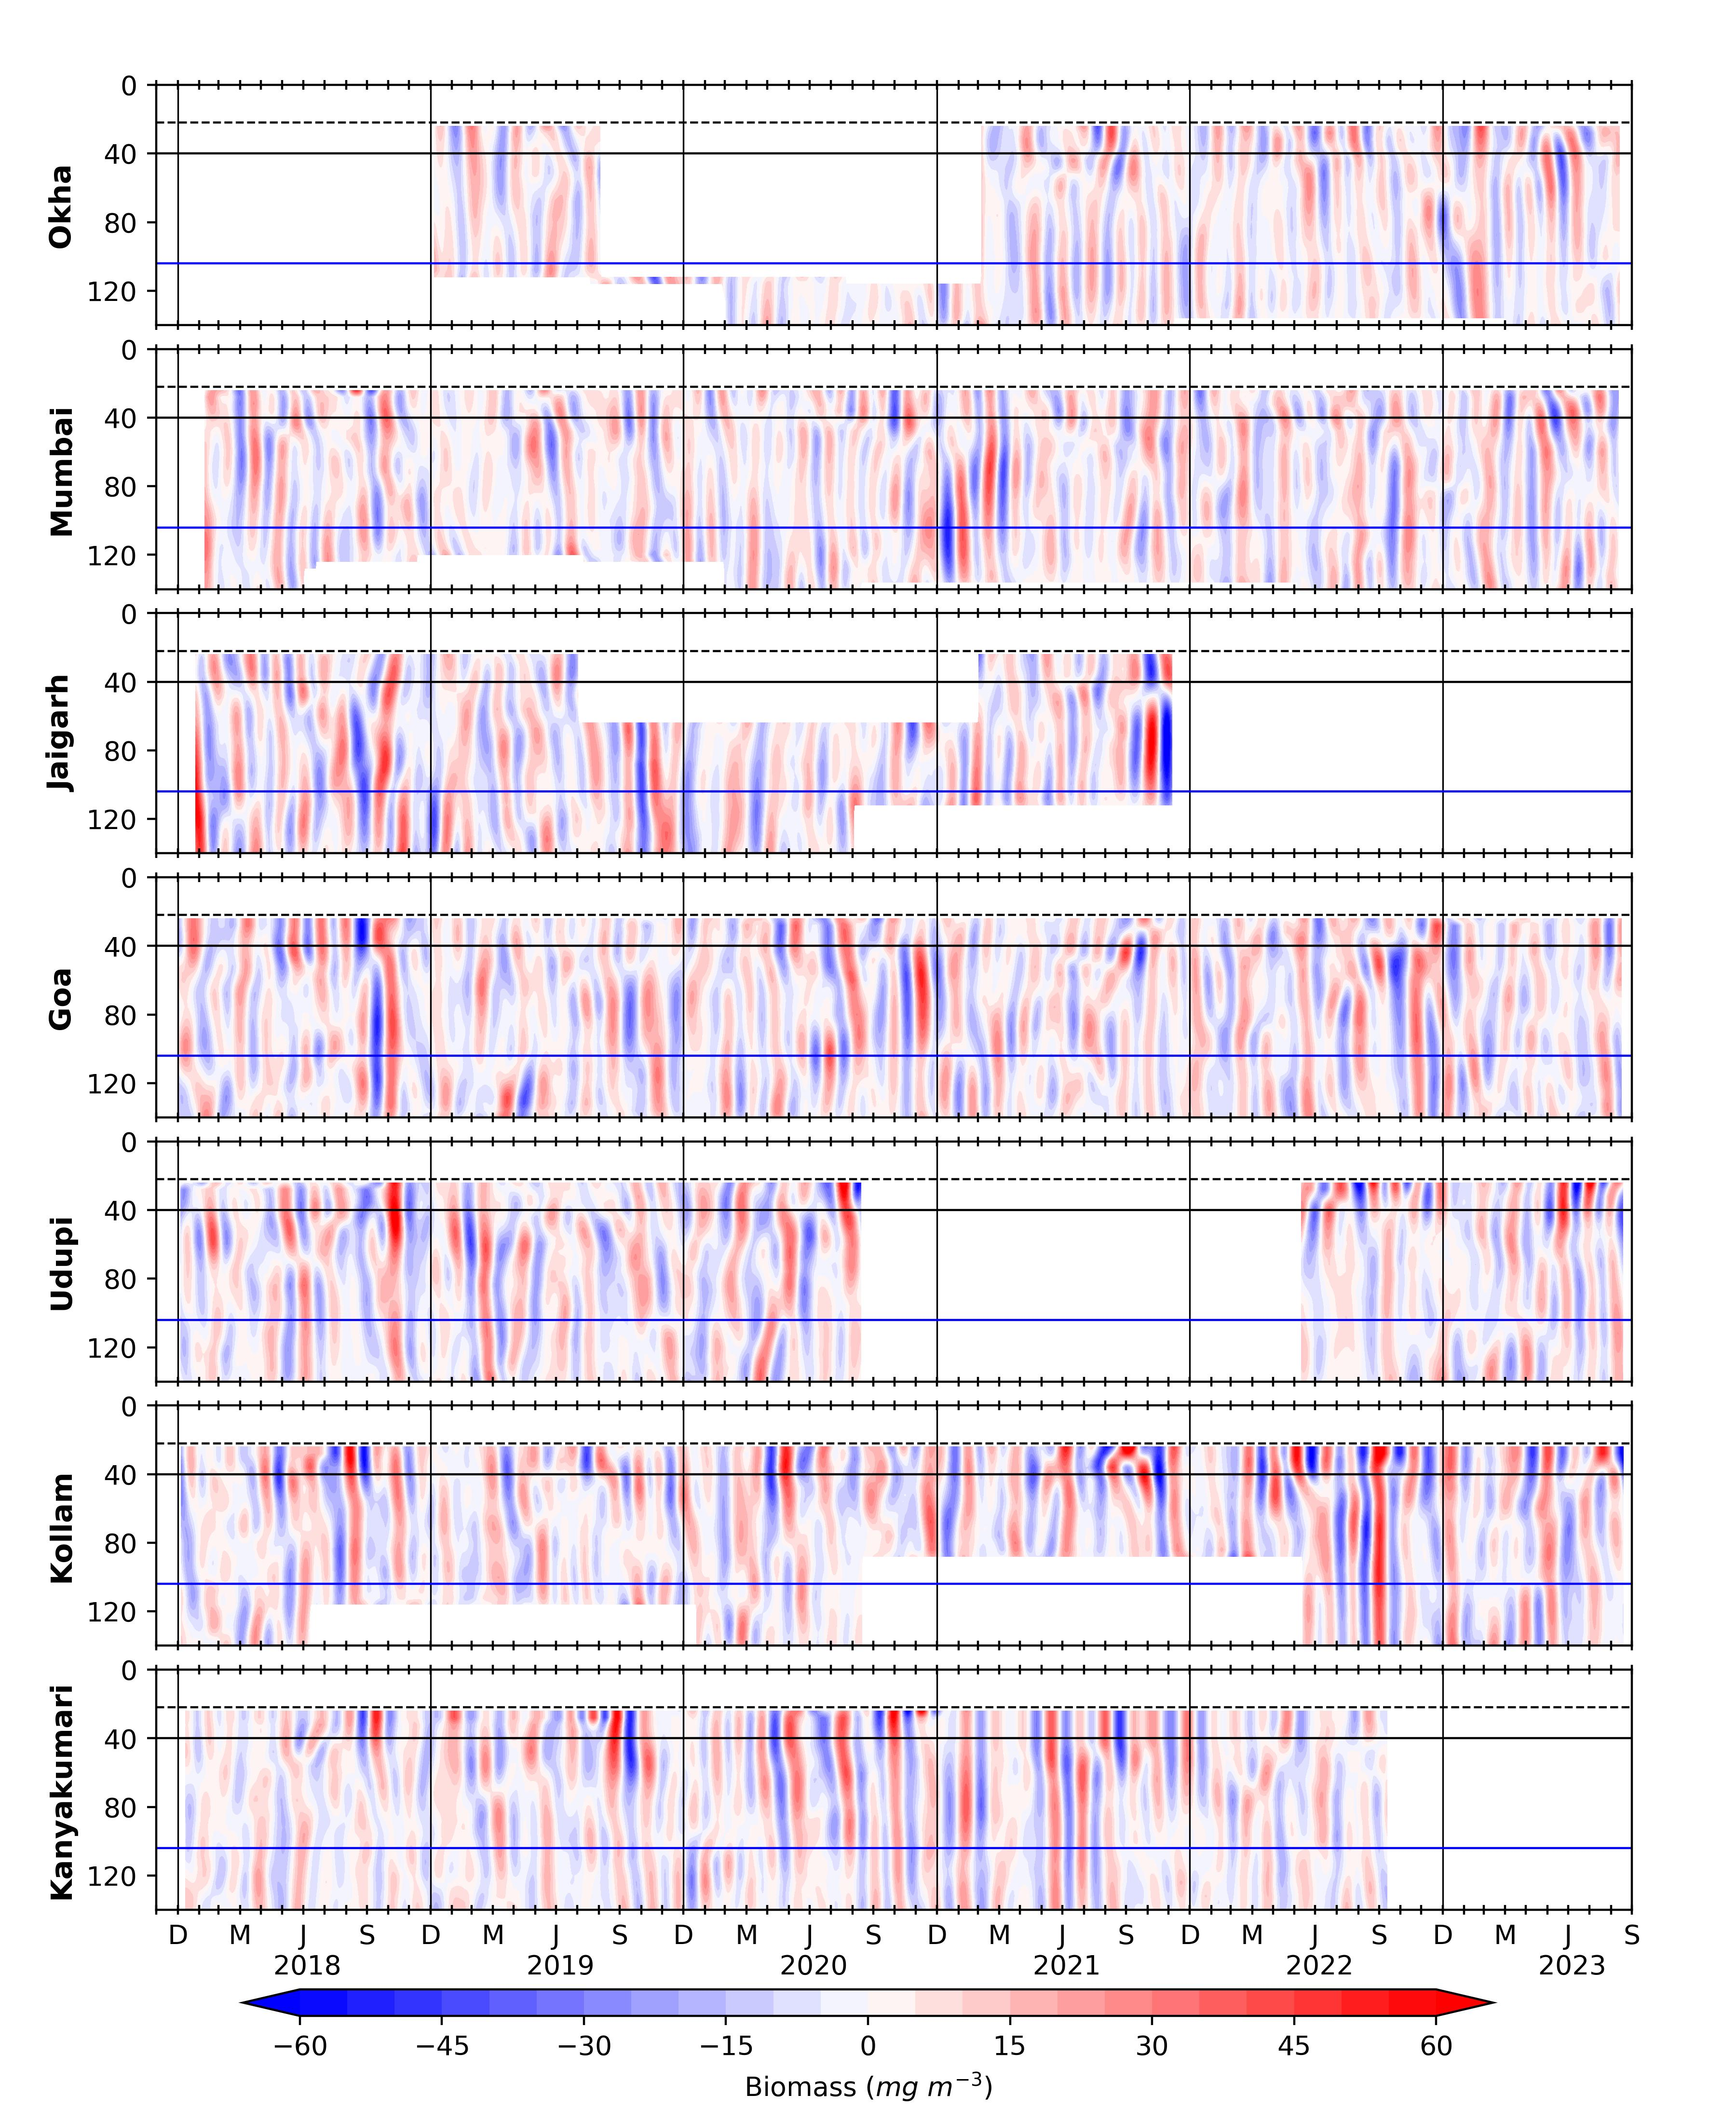
\includegraphics[width=\textwidth]{/media/scilab/disk_ranjan/works/backscatter_wc/figures/intraseasonal_30_90_181.jpeg} 
	\captionsetup{justification=justified,font=footnotesize,skip=0.05\baselineskip,width=\textwidth}
	\caption{Biomass variation found in the scale of 30 to 90 days  period (Intra-seasonal band as it is within a season) is obtained using a lanczos band pass filter. The horizontal black and blue lines is for 40 and 104 m respectively; vertical black lines separate the years. The dashed line at 22 m marks the top-depth of first bin i.e, 24 m.  Intraseasonal variability is seen throughout the record and the variability is stronger during August to November.}
	\label{fig:intraseasonal}
\end{figure}




\end{document}
